% ============================================================
%  main.tex — 《本科物理的数学基础》
%  编译方式: xelatex -> xelatex (两次编译)
% ============================================================
\documentclass[12pt,a4paper,openany]{ctexbook}

% --------------------------- 页面设置 ---------------------------
\usepackage[top=2.5cm,bottom=2.5cm,left=3cm,right=2.5cm,headheight=14.5pt]{geometry}
\usepackage{fancyhdr}
\pagestyle{fancy}
\fancyhf{}
\fancyhead[LE]{\leftmark}
\fancyhead[RO]{\rightmark}
\fancyfoot[C]{\thepage}
\renewcommand{\chaptermark}[1]{\markboth{\thechapter.\ #1}{}}

% --------------------------- 字体与编码 ---------------------------
\usepackage{fontspec}
\usepackage[UTF8]{ctex}
% 若系统无 Windows 字体，可取消下面注释改用默认字体
% \setCJKmainfont{SimSun}
% \setCJKsansfont{SimHei}
% \setCJKmonofont{FangSong}

% --------------------------- 数学宏包 ---------------------------
\usepackage{amsmath,amssymb,amsthm}
\usepackage{physics}          % 微分算符、括号、矢量
\usepackage{bm}               % 粗体数学符号
\usepackage{mathrsfs}         % 花体 \mathscr
\usepackage{upgreek}          % 直立体希腊字母
\DeclareMathOperator{\Arg}{Arg}   % 辐角主值
\DeclareMathOperator{\sinc}{sinc} % sinc 函数
\DeclareMathOperator{\erfc}{erfc} % 余误差函数

% --------------------------- 彩色与框 ---------------------------
\usepackage{xcolor}
\usepackage{tcolorbox}
\tcbuselibrary{skins,breakable}
\definecolor{insightbg}{RGB}{230,240,255}
\definecolor{insightframe}{RGB}{70,120,200}

% insight 环境 —— 物理直觉 / 物理洞察
% 用法: \begin{insight} 或 \begin{insight}[子标题]
\newtcolorbox[auto counter]{insight}[1][]{
    colback=insightbg,
    colframe=insightframe,
    coltitle=white,
    fonttitle=\bfseries,
    title={物理洞察~\thetcbcounter\ifstrempty{#1}{}{\ ---\ #1}},
    sharp corners,
    breakable,
    attach boxed title to top left={xshift=6mm,yshift=-2mm},
    boxed title style={colback=insightframe,sharp corners},
}

% --------------------------- 图形与浮动体 ---------------------------
\usepackage{graphicx}
\usepackage{float}
\usepackage{caption}
\usepackage{subcaption}
\graphicspath{{figures/}}

% --------------------------- 超链接与书签 ---------------------------
\usepackage[hidelinks]{hyperref}
\usepackage{bookmark}

% --------------------------- 定理环境 ---------------------------
\theoremstyle{definition}
\newtheorem{definition}{定义}[chapter]
\newtheorem{theorem}{定理}[chapter]
\newtheorem{lemma}{引理}[chapter]
\newtheorem{corollary}{推论}[chapter]
\theoremstyle{remark}
\newtheorem{remark}{注记}[chapter]
\newtheorem{example}{示例}[chapter]

% --------------------------- 代码/算法 ---------------------------
\usepackage{listings}
\lstset{
    basicstyle=\small\ttfamily,
    numbers=left,
    numberstyle=\tiny,
    frame=single,
    breaklines=true,
    backgroundcolor=\color{gray!5},
}

% --------------------------- 表格与其它 ---------------------------
\usepackage{booktabs}
\usepackage{cite}
\usepackage{enumitem}

% ============================================================
%  文档开始
% ============================================================
\begin{document}

%------------------ 封面 ------------------
\begin{titlepage}
    \centering
    \vspace*{4cm}
    \Huge\bfseries 本科物理的数学基础 \\[1cm]
    \Large Mathematical Foundations for Undergraduate Physics \\[2cm]
    \large 物理为血肉，数学为骨架 \\[0.5cm]
    \large — 在物理情景中理解数学，从数学推导中洞察物理 \\[3cm]
    \large \today \\[1cm]
    \large 初稿
    \vfill
\end{titlepage}

%------------------ 目录 ------------------
\tableofcontents
\clearpage

%------------------ 正文包含 ------------------
% ============================================================
%  第 1 章  坐标系、矢量分析与张量初步
%  教材完整版：~50页
% ============================================================

\chapter{坐标系、矢量分析与张量初步}

\section{本章概览与学习路线}

\subsection{本章在物理中的位置}

物理定律的数学表述离不开"空间"和"变化"两个概念。牛顿第二定律 $\mathbf{F}=m\mathbf{a}$ 中的加速度 $\mathbf{a}$ 是在某个坐标系中定义的二阶时间导数；麦克斯韦方程组是矢量场 $\mathbf{E}$ 和 $\mathbf{B}$ 在三维空间中的微积分关系；薛定谔方程中的哈密顿量 $\hat{H}$ 是线性空间上的厄米算符。所有这些物理理论，共享同一套数学语言——矢量分析、张量、线性空间。

本章构建这套语言。你将学到：

\begin{itemize}
  \item 如何在任意曲线坐标系中写出物理定律（拉梅系数）
  \item 矢量微积分的三大核心算符（梯度、散度、旋度）
  \item 连接局域与整体的积分定理（高斯、斯托克斯、格林）
  \item 矢量场分解的根本定理（亥姆霍兹分解）
  \item 保证物理定律坐标无关性的工具（张量）
  \item 量子力学的数学舞台（线性空间与厄米算符）
\end{itemize}

\subsection{前置知识}

阅读本章前，你应该熟悉：
\begin{itemize}
  \item 一元和多元微积分（偏导数、重积分、线面积分）
  \item 线性代数基础（矩阵乘法、行列式、本征值）
  \item 普通物理中的矢量运算（点积、叉积）
\end{itemize}

\subsection{学习路径建议}

\begin{itemize}
  \item \textbf{物理专业学生}：重点在 \S1.3--\S1.6（矢量分析）和 \S1.8--\S1.9（线性空间），这是电动力学和量子力学的直接预备。
  \item \textbf{数学专业学生}：重点在 \S1.7（张量）和 \S1.9（谱定理），这些是微分几何和泛函分析的入门。
  \item \textbf{工程专业学生}：重点在 \S1.3--\S1.6 和 \S1.7（转动惯量、应力张量），为连续介质力学打基础。
\end{itemize}

\section{引言：物理定律需要坐标系吗？}

\subsection{一个基本问题}

牛顿的推理是这样的：如果一个物体不受外力，"它将继续保持静止或匀速直线运动"。但问题在于——\textit{相对于谁静止？}

你在匀速行驶的火车上捡起一枚硬币，它做竖直直线运动（相对于火车），同时做抛物线运动（相对于地面）。两个描述都是正确的，但用的坐标系不同。这个看似平凡的事实引出了一个深刻的物理原理：\textbf{物理定律的形式在所有惯性系中相同}（伽利略相对性原理）。

但数学上，"同一物理定律在不同坐标系下形式不变"是什么意思？以梯度为例：
\[
\nabla f = \frac{\partial f}{\partial x}\mathbf{e}_x + \frac{\partial f}{\partial y}\mathbf{e}_y + \frac{\partial f}{\partial z}\mathbf{e}_z
\]
在直角坐标中是这样的形式。但在球坐标中，我们将会看到
\[
\nabla f = \frac{\partial f}{\partial r}\mathbf{e}_r + \frac{1}{r}\frac{\partial f}{\partial\theta}\mathbf{e}_\theta + \frac{1}{r\sin\theta}\frac{\partial f}{\partial\phi}\mathbf{e}_\phi .
\]

看起来不同，但\textbf{物理量是同一个 $\nabla f$}，只是表达方式不同。理解这种"不同写法代表同一物理量"的能力，是本章的第一个核心目标。

\subsection{本章的逻辑主线}

\begin{center}
\fbox{\parbox{0.85\textwidth}{
\textbf{物理问题 $\to$ 选择坐标系 $\to$ 拉梅系数描述几何 $\to$ 微分算符表达定律 $\to$ 积分定理揭示守恒 $\to$ 张量保证协变 $\to$ 线性空间抽象 $\to$ 本征值连接可观测量}
}}
\end{center}

这条线索将在后续所有章节中被反复强化。每当你在第 2 章遇到复变积分、在第 3 章遇到傅里叶变换、在第 4 章遇到 PDE，你都会回到本章建立的框架——\textbf{物理对称性决定数学形式，数学形式揭示物理规律}。

\section{正交曲线坐标系与拉梅系数}

\subsection{为什么不能只用直角坐标？}

直角坐标 $(x,y,z)$ 是可以描述任何点的，但在物理学中，我们遇到的绝大多数问题都具有某种对称性：

\begin{itemize}
  \item \textbf{球对称}：中心力场、氢原子、点电荷的电场
  \item \textbf{柱对称}：无限长导线、圆波导、光纤
  \item \textbf{抛物线对称}：匀强电场中的带电粒子轨迹
\end{itemize}

如果将一个球对称问题强制塞进直角坐标，边界条件会变得极其复杂。例如球的表面 $x^2+y^2+z^2=R^2$ 需要同时约束三个坐标。而在球坐标中，边界只是简洁的 $r=R$。

\textbf{基本原则：让坐标面与物理边界重合。}

\subsection{从直角坐标到一般曲线坐标}

设三维欧氏空间中有一组新的坐标 $(q_1,q_2,q_3)$，它们与直角坐标 $(x,y,z)$ 之间的变换关系为
\begin{equation}
x = x(q_1,q_2,q_3),\quad
y = y(q_1,q_2,q_3),\quad
z = z(q_1,q_2,q_3),
\label{eq:general_transform}
\end{equation}
其中变换函数是光滑的，且雅可比矩阵 $\partial(x,y,z)/\partial(q_1,q_2,q_3)$ 在讨论区域内非奇异（保证变换可逆）。

\subsection{拉梅系数的几何意义}

考虑一个无限小的位移：
\[
\dd\mathbf{r} = \frac{\partial\mathbf{r}}{\partial q_1}\dd q_1
+ \frac{\partial\mathbf{r}}{\partial q_2}\dd q_2
+ \frac{\partial\mathbf{r}}{\partial q_3}\dd q_3 .
\]

每个 $\partial\mathbf{r}/\partial q_i$ 是一个矢量，指向 $q_i$ 增加的方向。其长度
\[
h_i = \left|\frac{\partial\mathbf{r}}{\partial q_i}\right|,\qquad i=1,2,3
\]
称为\textbf{拉梅系数 (Lamé coefficients)}。沿 $q_i$ 方向的单位矢量为
\[
\mathbf{e}_i = \frac{1}{h_i}\frac{\partial\mathbf{r}}{\partial q_i}.
\]

\textbf{弧长平方：}
\[
\dd s^2 = \dd\mathbf{r}\cdot\dd\mathbf{r}
= \sum_{i,j} \frac{\partial\mathbf{r}}{\partial q_i}\cdot\frac{\partial\mathbf{r}}{\partial q_j}\dd q_i\dd q_j .
\]

如果 $\mathbf{e}_i\cdot\mathbf{e}_j = \delta_{ij}$（即坐标线处处正交），则交叉项（$i\neq j$ 的项）消失：
\[
\boxed{\;\dd s^2 = h_1^2\dd q_1^2 + h_2^2\dd q_2^2 + h_3^2\dd q_3^2\;}.
\label{eq:metric_line_element}
\]

这就是\textbf{正交曲线坐标系}的定义。

\begin{example}[完整推导：三种坐标系的拉梅系数]
\textbf{(1) 柱坐标 $(\rho,\phi,z)$}
\[
x = \rho\cos\phi,\quad y = \rho\sin\phi,\quad z = z.
\]

计算偏导：
\[
\frac{\partial\mathbf{r}}{\partial\rho} = (\cos\phi,\sin\phi,0),\quad
\frac{\partial\mathbf{r}}{\partial\phi} = (-\rho\sin\phi,\rho\cos\phi,0),\quad
\frac{\partial\mathbf{r}}{\partial z} = (0,0,1).
\]

取模：
\[
h_\rho = 1,\quad h_\phi = \sqrt{\rho^2\sin^2\phi+\rho^2\cos^2\phi} = \rho,\quad h_z = 1.
\]

弧长元：
\[
\dd s^2 = \dd\rho^2 + \rho^2\dd\phi^2 + \dd z^2.
\]

\textbf{(2) 球坐标 $(r,\theta,\phi)$}
\[
x = r\sin\theta\cos\phi,\quad y = r\sin\theta\sin\phi,\quad z = r\cos\theta.
\]

偏导数：
\begin{align*}
\frac{\partial\mathbf{r}}{\partial r} &= (\sin\theta\cos\phi,\sin\theta\sin\phi,\cos\theta),\\
\frac{\partial\mathbf{r}}{\partial\theta} &= (r\cos\theta\cos\phi,r\cos\theta\sin\phi,-r\sin\theta),\\
\frac{\partial\mathbf{r}}{\partial\phi} &= (-r\sin\theta\sin\phi,r\sin\theta\cos\phi,0).
\end{align*}

取模：
\[
h_r = 1,\quad h_\theta = r,\quad h_\phi = r\sin\theta.
\]

弧长元：
\[
\dd s^2 = \dd r^2 + r^2\dd\theta^2 + r^2\sin^2\theta\,\dd\phi^2.
\]

\textbf{(3) 抛物线坐标 $(\xi,\eta,\phi)$}
\[
x = \xi\eta\cos\phi,\quad y = \xi\eta\sin\phi,\quad z = \frac12(\xi^2-\eta^2).
\]

拉梅系数：
\[
h_\xi = h_\eta = \sqrt{\xi^2+\eta^2},\quad h_\phi = \xi\eta.
\]

这组坐标在带电粒子在匀强电场中的运动问题中极为有用。
\end{example}

\begin{insight}[拉梅系数 = 局部标尺]
拉梅系数的物理图像非常直观：当你沿 $q_i$ 方向走一个坐标步 $\dd q_i$ 时，实际在三维空间中移动了 $h_i\dd q_i$ 这么远。因此 $h_i$ 就是"坐标步长到实际距离的换算因子"。在球坐标中，沿 $\theta$ 方向走 $\dd\theta$ 对应实际距离 $r\dd\theta$（$h_\theta=r$），沿 $\phi$ 方向走 $\dd\phi$ 对应实际距离 $r\sin\theta\,\dd\phi$（$h_\phi=r\sin\theta$）。你可以把这个想象成地球上的经纬度——经度一度对应的地面距离取决于你所在的纬度。
\end{insight}

\section{微分算符在曲线坐标系中的形式}

\subsection{梯度}

梯度 $\nabla f$ 的物理定义是"方向导数最大的方向"及其"最大变化率"。在曲线坐标中，沿 $q_i$ 方向的方向导数为 $(1/h_i)\partial f/\partial q_i$，因此
\[
\boxed{\;\nabla f = \sum_{i=1}^3 \frac{1}{h_i}\frac{\partial f}{\partial q_i}\mathbf{e}_i\;}.
\label{eq:grad_curvilinear}
\]

\subsection{散度}

散度 $\nabla\cdot\mathbf{A}$ 的物理定义是"单位体积的通量"。考虑一个由坐标线围成的无限小曲边六面体，穿过两个相对面的净通量差给出：
\[
\boxed{\;
\nabla\cdot\mathbf{A}
= \frac{1}{h_1h_2h_3}\sum_{i=1}^3
\frac{\partial}{\partial q_i}\left(\frac{h_1h_2h_3}{h_i}A_i\right)
\;}.
\label{eq:div_curvilinear}
\]

\begin{example}[柱坐标中的散度]
$h_\rho=1,\;h_\phi=\rho,\;h_z=1$，$h_1h_2h_3 = \rho$。
\begin{align*}
\nabla\cdot\mathbf{A}
&= \frac{1}{\rho}\left[
\frac{\partial}{\partial\rho}(\rho A_\rho)
+ \frac{\partial}{\partial\phi}(A_\phi)
+ \frac{\partial}{\partial z}(\rho A_z)
\right] \\
&= \frac{1}{\rho}\frac{\partial}{\partial\rho}(\rho A_\rho)
+ \frac{1}{\rho}\frac{\partial A_\phi}{\partial\phi}
+ \frac{\partial A_z}{\partial z}.
\end{align*}
\end{example}

\subsection{旋度}

旋度 $\nabla\times\mathbf{A}$ 的物理定义是"单位面积的最大环量"。同样从六面体的面环量出发：
\[
\boxed{\;
\nabla\times\mathbf{A}
= \sum_{i=1}^3\frac{1}{h_jh_k}
\left[\frac{\partial}{\partial q_j}(h_kA_k)-\frac{\partial}{\partial q_k}(h_jA_j)\right]\mathbf{e}_i
\;}.
\label{eq:curl_curvilinear}
\]

其中 $(i,j,k)$ 取 $(1,2,3)$ 的循环置换。

\begin{example}[球坐标中的旋度]
\begin{align*}
\nabla\times\mathbf{A}
&= \frac{1}{r\sin\theta}\left[
\frac{\partial}{\partial\theta}(\sin\theta A_\phi)
- \frac{\partial A_\theta}{\partial\phi}
\right]\mathbf{e}_r \\
&\quad + \frac{1}{r}\left[
\frac{1}{\sin\theta}\frac{\partial A_r}{\partial\phi}
- \frac{\partial}{\partial r}(r A_\phi)
\right]\mathbf{e}_\theta \\
&\quad + \frac{1}{r}\left[
\frac{\partial}{\partial r}(r A_\theta)
- \frac{\partial A_r}{\partial\theta}
\right]\mathbf{e}_\phi .
\end{align*}
\end{example}

\subsection{拉普拉斯算子}

拉普拉斯算子 $\nabla^2 f = \nabla\cdot(\nabla f)$，将梯度公式代入散度公式：
\[
\boxed{\;
\nabla^2 f = \frac{1}{h_1h_2h_3}\sum_{i=1}^3
\frac{\partial}{\partial q_i}\left(\frac{h_1h_2h_3}{h_i^2}
\frac{\partial f}{\partial q_i}\right)
\;}.
\label{eq:laplacian_curvilinear}
\]

\begin{example}[完整算例：氢原子的拉普拉斯算子]
氢原子的薛定谔方程在球坐标中写为：
\[
-\frac{\hbar^2}{2m}\nabla^2\psi - \frac{e^2}{4\pi\varepsilon_0 r}\psi = E\psi.
\]

代入 $h_r=1,\;h_\theta=r,\;h_\phi=r\sin\theta$：
\begin{align*}
\nabla^2\psi &= \frac{1}{r^2}\frac{\partial}{\partial r}\left(r^2\frac{\partial\psi}{\partial r}\right)
+ \frac{1}{r^2\sin\theta}\frac{\partial}{\partial\theta}\left(\sin\theta\frac{\partial\psi}{\partial\theta}\right)
+ \frac{1}{r^2\sin^2\theta}\frac{\partial^2\psi}{\partial\phi^2} \\
&= \frac{1}{r^2}\frac{\partial}{\partial r}\left(r^2\frac{\partial\psi}{\partial r}\right)
- \frac{\hat{L}^2}{\hbar^2 r^2}\psi,
\end{align*}
其中 $\hat{L}^2 = -\hbar^2\left[\frac{1}{\sin\theta}\frac{\partial}{\partial\theta}\left(\sin\theta\frac{\partial}{\partial\theta}\right) + \frac{1}{\sin^2\theta}\frac{\partial^2}{\partial\phi^2}\right]$ 是角动量平方算符。

这正是分离变量法的出发点——径向部分和角向部分自然分离，因为拉普拉斯算子的球坐标形式就包含了这种结构。
\end{example}

\begin{example}[完整算例：点电荷电场的散度验证]
点电荷 $q$ 在球坐标中的电场 $\mathbf{E} = \frac{q}{4\pi\varepsilon_0 r^2}\mathbf{e}_r$。

用散度公式验证 $\nabla\cdot\mathbf{E}=0$（$r>0$）：
\begin{align*}
\nabla\cdot\mathbf{E}
&= \frac{1}{r^2}\frac{\partial}{\partial r}\left(r^2 E_r\right) \\
&= \frac{1}{r^2}\frac{\partial}{\partial r}\left(r^2\cdot\frac{q}{4\pi\varepsilon_0 r^2}\right) \\
&= \frac{1}{r^2}\frac{\partial}{\partial r}\left(\frac{q}{4\pi\varepsilon_0}\right) = 0.
\end{align*}
关键点：$r^2 E_r = q/(4\pi\varepsilon_0)$ 是常数——这正是因为 $\mathbf{E}\propto 1/r^2$。如果电场按 $1/r^{2+\varepsilon}$ 衰减，散度就不为零了。这说明\textbf{库仑平方反比律直接等价于 $\nabla\cdot\mathbf{E}=0$（除点电荷外）}。
\end{example}

\section{Levi-Civita 符号与矢量代数}

\subsection{为什么需要一种新的符号？}

矢量分析中有大量恒等式，用分量展开证明非常冗长。例如
\[
\nabla\times(\nabla\times\mathbf{A}) = \nabla(\nabla\cdot\mathbf{A}) - \nabla^2\mathbf{A},
\]
在电磁学中几乎每天都要用到。如果用分量展开硬算，三个方向共 9 项。而用指标符号只需 3 行。

更重要的是，指标符号是张量分析的入门钥匙——后续的狭义相对论和广义相对论将大量使用这种语言。

\subsection{定义}

\textbf{Levi-Civita 符号} $\epsilon_{ijk}$（也称为排列符号或反对称符号）定义为：
\[
\epsilon_{ijk} =
\begin{cases}
+1, & (i,j,k) \text{ 为 } (1,2,3)\text{ 的偶排列},\\
-1, & (i,j,k) \text{ 为 }(1,2,3)\text{ 的奇排列},\\
0, & \text{有重复指标}.
\end{cases}
\]

偶排列：$(1,2,3), (2,3,1), (3,1,2)$。
奇排列：$(3,2,1), (1,3,2), (2,1,3)$。

\subsection{用 \texorpdfstring{$\epsilon_{ijk}$}{εijk} 表示叉积和行列式}

\textbf{叉积：}
\[
(\mathbf{A}\times\mathbf{B})_i = \epsilon_{ijk}A_jB_k,
\]
其中重复指标 $j,k$ 自动求和（\textbf{爱因斯坦求和约定}）。

\textbf{行列式：}
\[
\det\begin{pmatrix}
a_{11} & a_{12} & a_{13}\\
a_{21} & a_{22} & a_{23}\\
a_{31} & a_{32} & a_{33}
\end{pmatrix}
= \epsilon_{ijk}a_{1i}a_{2j}a_{3k}.
\]

\subsection{最重要的恒等式：\texorpdfstring{$\epsilon$-$\delta$}{ε-δ} 关系}

\[
\boxed{\;\epsilon_{ijk}\epsilon_{ilm} = \delta_{jl}\delta_{km} - \delta_{jm}\delta_{kl}\;}.
\label{eq:epsilon_delta}
\]

这里对 $i$ 求和。理解这个公式：
\begin{itemize}
\item 左边：两个 Levi-Civita 符号的乘积，对共同指标 $i$ 求和。
\item 右边：两个 Kronecker $\delta$ 的乘积之差。
\item 口诀：\textbf{"积的差"}——$\delta_{jl}\delta_{km}$ 减交换 $l,m$ 的 $\delta_{jm}\delta_{kl}$。
\end{itemize}

\subsection{恒等式的指标法证明}

\begin{example}[三重积 $\mathbf{A}\times(\mathbf{B}\times\mathbf{C})$]
\textbf{目标：} $\mathbf{A}\times(\mathbf{B}\times\mathbf{C}) = \mathbf{B}(\mathbf{A}\cdot\mathbf{C}) - \mathbf{C}(\mathbf{A}\cdot\mathbf{B})$。

第 $i$ 分量：
\begin{align*}
[\mathbf{A}\times(\mathbf{B}\times\mathbf{C})]_i
&= \epsilon_{ijk}A_j(\mathbf{B}\times\mathbf{C})_k \\
&= \epsilon_{ijk}A_j\epsilon_{klm}B_lC_m \\
&= \epsilon_{kij}\epsilon_{klm}A_jB_lC_m \\
&= (\delta_{il}\delta_{jm} - \delta_{im}\delta_{jl})A_jB_lC_m.
\end{align*}
展开两项：
\begin{itemize}
\item $\delta_{il}\delta_{jm}A_jB_lC_m = A_jB_iC_j = B_i(\mathbf{A}\cdot\mathbf{C})$。
\item $\delta_{im}\delta_{jl}A_jB_lC_m = A_jB_jC_i = C_i(\mathbf{A}\cdot\mathbf{B})$。
\end{itemize}
所以 $[\mathbf{A}\times(\mathbf{B}\times\mathbf{C})]_i = B_i(\mathbf{A}\cdot\mathbf{C}) - C_i(\mathbf{A}\cdot\mathbf{B})$，即矢量形式。$\square$
\end{example}

\begin{example}[三重积 $(\mathbf{A}\times\mathbf{B})\times\mathbf{C}$]
\[
(\mathbf{A}\times\mathbf{B})\times\mathbf{C} = \mathbf{B}(\mathbf{A}\cdot\mathbf{C}) - \mathbf{A}(\mathbf{B}\cdot\mathbf{C}).
\]
第 $i$ 分量：
\begin{align*}
[(\mathbf{A}\times\mathbf{B})\times\mathbf{C}]_i
&= \epsilon_{ijk}(\mathbf{A}\times\mathbf{B})_jC_k \\
&= \epsilon_{ijk}\epsilon_{jlm}A_lB_mC_k \\
&= -\epsilon_{jik}\epsilon_{jlm}A_lB_mC_k \\
&= -(\delta_{il}\delta_{km} - \delta_{im}\delta_{kl})A_lB_mC_k \\
&= -A_iB_kC_k + A_kB_iC_k \\
&= B_i(\mathbf{A}\cdot\mathbf{C}) - A_i(\mathbf{B}\cdot\mathbf{C}).
\end{align*}
注意结果中 $\mathbf{A}$ 和 $\mathbf{C}$ 的位置与第一个三重积不同——叉积不满足结合律！$\square$
\end{example}

\begin{example}[证明 $\nabla\times(\nabla f) = 0$]
\begin{align*}
[\nabla\times(\nabla f)]_i
&= \epsilon_{ijk}\partial_j\partial_k f.
\end{align*}
由于 $\partial_j\partial_k f = \partial_k\partial_j f$（混合偏导与次序无关），而 $\epsilon_{ijk}$ 关于 $j,k$ 反对称，求和为零。$\square$
\end{example}

\begin{example}[证明 $\nabla\cdot(\nabla\times\mathbf{A}) = 0$]
\begin{align*}
\nabla\cdot(\nabla\times\mathbf{A})
&= \partial_i(\epsilon_{ijk}\partial_j A_k) \\
&= \epsilon_{ijk}\partial_i\partial_j A_k.
\end{align*}
同样 $\partial_i\partial_j = \partial_j\partial_i$ 关于 $i,j$ 对称，$\epsilon_{ijk}$ 关于 $i,j$ 反对称，结果为零。$\square$
\end{example}

\subsection{物理洞察：为什么 \texorpdfstring{$\epsilon_{ijk}$}{εijk} 这么有用？}

物理定律经常涉及叉积。力矩 $\bm{\tau} = \mathbf{r}\times\mathbf{F}$，洛伦兹力 $\mathbf{F}=q\mathbf{v}\times\mathbf{B}$，角动量 $\mathbf{L} = \mathbf{r}\times\mathbf{p}$。用指标符号，这些可以统一处理。

更重要的是，$\epsilon_{ijk}$ 是三维空间中"定向体积元"的自然表达——它告诉我们坐标变换是否改变定向（手性）。这正是后续学习中区分\textbf{轴矢量}（如 $\mathbf{B}$）和\textbf{极矢量}（如 $\mathbf{r}$）的数学基础。

\subsection{应避免的常见错误}

\begin{itemize}
  \item \textbf{求和指标混淆}：$\epsilon_{ijk}A_jB_k$ 中 $j,k$ 是哑指标，可以改名。但哑指标在同一项中恰好出现两次——例如 $\epsilon_{iji}A_jB_i$ 中 $i$ 出现了三次（$\epsilon$ 的第一个、第三个位置以及 $B_i$ 中），这样的写法是非法的！
  \item \textbf{$\epsilon$ 乘积次序}：$\epsilon_{ijk}\epsilon_{ilm}$ 对 $i$ 求和；$\epsilon_{jik}\epsilon_{ilm} = -\epsilon_{ijk}\epsilon_{ilm}$。
  \item \textbf{符号误判}：$(1,3,2)$ 是奇排列（一次交换），$\epsilon_{132} = -1$。
\end{itemize}

\section{三大积分定理}

\subsection{从局域到整体}

微分形式的物理定律（如 $\nabla\cdot\mathbf{E}=\rho/\varepsilon_0$）告诉我们每一点的场行为。但实验测量往往是整体的——我们测量穿过线圈的总磁通量，而不是每一点的 $\mathbf{B}$。积分定理就是连接这两种描述的桥梁。

\subsection{高斯散度定理}

\begin{theorem}[高斯定理]
对于光滑矢量场 $\mathbf{F}$ 和由光滑曲面 $\partial V$ 围成的区域 $V$，
\[
\boxed{\;\int_V (\nabla\cdot\mathbf{F})\,\dd V = \oint_{\partial V} \mathbf{F}\cdot\dd\mathbf{S}\;}.
\label{eq:gauss_div}
\]

\textbf{证明思路（一维启示）：} 一维情形下，$\int_a^b f'(x)\,\dd x = f(b)-f(a)$——内部导数的积分等于边界函数值之差。高斯定理正是这个基本定理在三维的推广。

左端是场在体积内的"源"的总强度；右端是穿过边界的"通量"。方程告诉我们：\textbf{体积内源的强度之和等于边界面流出的通量之和}。
\end{theorem}

\begin{insight}[高斯定理与电荷守恒]
在电动力学中，电流连续性方程为 $\nabla\cdot\mathbf{J} + \partial\rho/\partial t = 0$。对体积 $V$ 积分并用高斯定理：
\[
\oint_{\partial V}\mathbf{J}\cdot\dd\mathbf{S} = -\frac{\dd}{\dd t}\int_V\rho\,\dd V = -\frac{\dd Q_{\text{内}}}{\dd t}.
\]
这说的是：流出边界的电流等于内部电荷的减少率。这就是电荷守恒定律的积分形式。
\end{insight}

\begin{example}[完整算例：验证高斯定理]
取 $\mathbf{F} = (x^2, yz, z)$，$V$ 为单位立方体 $0\leq x,y,z\leq 1$。

\textbf{直接计算散度的体积分：}
\[
\nabla\cdot\mathbf{F} = 2x + z + 1.
\]
\[
\int_V \nabla\cdot\mathbf{F}\,\dd V = \int_0^1\int_0^1\int_0^1 (2x+z+1)\,\dd x\dd y\dd z = \frac52.
\]

\textbf{计算面积分：} 立方体有 6 个面。以 $x=1$ 面（法向 $\mathbf{e}_x$）为例：
\[
\int_{x=1} \mathbf{F}\cdot\dd\mathbf{S} = \int_0^1\int_0^1 (1^2)\,\dd y\dd z = 1.
\]
$x=0$ 面（法向 $-\mathbf{e}_x$）：
\[
\int_{x=0} \mathbf{F}\cdot\dd\mathbf{S} = \int_0^1\int_0^1 (0)\,\dd y\dd z = 0.
\]
类似计算其余 4 个面并求和，总面积分也为 $5/2$。高斯定理成立。$\square$
\end{example}

\subsection{斯托克斯定理}

\begin{theorem}[斯托克斯定理]
对于光滑矢量场 $\mathbf{F}$ 和以定向曲线 $\partial S$ 为边界的曲面 $S$，
\[
\boxed{\;\int_S (\nabla\times\mathbf{F})\cdot\dd\mathbf{S} = \oint_{\partial S} \mathbf{F}\cdot\dd\mathbf{l}\;}.
\label{eq:stokes}
\]

物理意义：曲面上的旋度通量等于边界上的环量。
\end{theorem}

\begin{example}[完整算例：斯托克斯定理计算环量]
$\mathbf{F} = (-y, x, 0)$，求沿 $x^2+y^2=R^2$（$z=0$）的环量。

\textbf{直接参数化：}
$\mathbf{r}(\theta) = (R\cos\theta, R\sin\theta, 0)$，$\dd\mathbf{l}=(-R\sin\theta, R\cos\theta, 0)\,\dd\theta$。
\[
\oint\mathbf{F}\cdot\dd\mathbf{l} = \int_0^{2\pi} (R^2\sin^2\theta+R^2\cos^2\theta)\,\dd\theta = 2\pi R^2.
\]

\textbf{斯托克斯定理：}
$\nabla\times\mathbf{F} = (0,0,2)$。
取圆盘 $S$（法向 $\mathbf{e}_z$）：
\[
\int_S (\nabla\times\mathbf{F})\cdot\dd\mathbf{S} = 2\cdot(\pi R^2) = 2\pi R^2.
\]
一致。注意这个结果具有几何意义：由于 $\nabla\times\mathbf{F}$ 是常数，环量正比于圆盘面积 $\pi R^2$，即正比于 $R^2$——这正是斯托克斯定理告诉我们的。
\end{example}

\subsection{格林恒等式}

由高斯定理直接导出两组恒等式，它们在 PDE 理论中极为重要。

设 $f,g$ 为光滑标量函数。

\textbf{第一格林恒等式：}
\[
\int_V (f\nabla^2 g + \nabla f\cdot\nabla g)\,\dd V = \oint_{\partial V} f\nabla g\cdot\dd\mathbf{S}.
\label{eq:green1}
\]

\textbf{第二格林恒等式：}
\[
\int_V (f\nabla^2 g - g\nabla^2 f)\,\dd V = \oint_{\partial V} (f\nabla g - g\nabla f)\cdot\dd\mathbf{S}.
\label{eq:green2}
\]

\textbf{推导：} 从高斯定理出发，令 $\mathbf{F} = f\nabla g$：
\[
\nabla\cdot(f\nabla g) = \nabla f\cdot\nabla g + f\nabla^2 g.
\]
代入高斯定理即得第一恒等式。交换 $f,g$ 后相减得第二恒等式。

\begin{insight}[格林恒等式的物理意义]
格林恒等式在电动力学中被用来证明\textbf{格林互易定理}：若 $\phi_1$ 由电荷分布 $\rho_1$ 产生，$\phi_2$ 由 $\rho_2$ 产生，则
\[
\int\rho_1\phi_2\,\dd V = \int\rho_2\phi_1\,\dd V.
\]
这个对称性关系在电容矩阵计算和电像法中非常有用。
\end{insight}

\subsection{亥姆霍兹分解}

\begin{theorem}[亥姆霍兹定理]
任何在无穷远处衰减足够快的光滑矢量场 $\mathbf{F}$ 可以唯一分解为一个无旋场和一个无散场之和：
\[
\boxed{\;\mathbf{F} = -\nabla\phi + \nabla\times\mathbf{A}\;},
\label{eq:helmholtz}
\]
其中
\[
\phi(\mathbf{r}) = \frac{1}{4\pi}\int\frac{\nabla'\cdot\mathbf{F}(\mathbf{r}')}{|\mathbf{r}-\mathbf{r}'|}\,\dd V',\qquad
\mathbf{A}(\mathbf{r}) = \frac{1}{4\pi}\int\frac{\nabla'\times\mathbf{F}(\mathbf{r}')}{|\mathbf{r}-\mathbf{r}'|}\,\dd V'.
\]

{\bfseries 这个定理为什么重要？}
\begin{itemize}
\item 在电动力学中，电场 $\mathbf{E} = -\nabla\phi - \partial\mathbf{A}/\partial t$——把 $\mathbf{E}$ 分解为库仑场（无旋）和感应场（无散在规范下）。
\item 在流体力学中，速度 $\mathbf{v} = -\nabla\phi + \nabla\times\bm{\psi}$——纵波（声波）和横波（剪切波）的分解。
\item 在地震学中，P 波（纵波，$\nabla\times\mathbf{u}=0$）和 S 波（横波，$\nabla\cdot\mathbf{u}=0$）的分离。
\end{itemize}
\end{theorem}

\section{张量初步}

\subsection{从矢量到张量：一个必要的推广}

矢量 $\mathbf{v}$ 有 3 个分量，描述力、速度等。但有些物理量需要更复杂的结构：
\begin{itemize}
  \item \textbf{转动惯量} $\mathbf{I}$：把角速度 $\bm{\omega}$ 映射为角动量 $\mathbf{L}$，$\mathbf{L} = \mathbf{I}\bm{\omega}$。如果 $\bm{\omega}$ 不沿主轴，$\mathbf{L}$ 与 $\bm{\omega}$ 方向不同。
  \item \textbf{应力} $\sigma_{ij}$：$i$ 方向的力作用在法向为 $j$ 的面上，9 个分量。
  \item \textbf{电磁场} $F^{\mu\nu}$：电场和磁场统一为四维反对称张量。
\end{itemize}

这些量的共同特征：它们给出了一个\textbf{线性映射}——把一个矢量（或更一般的张量）映射为另一个矢量（或张量）。这个映射在坐标变换下必须满足确定的变换规则，这就是张量的本质。

\subsection{张量的变换规则}

设 $V$ 是一个 $n$ 维矢量空间，$\{e_i\}$ 和 $\{e'_i\}$ 是两组基，变换矩阵为 $\Lambda^i_j = \partial x'^i/\partial x^j$。

\textbf{逆变矢量：} 分量与基矢反向变换，$V'^i = \Lambda^i_j V^j$。
\textbf{协变矢量：} 分量与基矢同向变换，$V'_i = (\Lambda^{-1})^j_i V_j$。

\textbf{$(p,q)$ 型张量：} 有 $p$ 个逆变指标和 $q$ 个协变指标，变换规则为
\[
T'^{\mu_1\cdots\mu_p}_{\nu_1\cdots\nu_q}
= \Lambda^{\mu_1}_{\alpha_1}\cdots\Lambda^{\mu_p}_{\alpha_p}
(\Lambda^{-1})^{\beta_1}_{\nu_1}\cdots(\Lambda^{-1})^{\beta_q}_{\nu_q}
\;T^{\alpha_1\cdots\alpha_p}_{\beta_1\cdots\beta_q}.
\]

\textbf{零阶张量 = 标量}，\textbf{一阶张量 = 矢量}，\textbf{二阶张量 = 矩阵（但需满足变换规则）}。

\subsection{度规张量}

曲线坐标中的弧长平方是物理不变量，可写为
\[
\dd s^2 = g_{\mu\nu}\,\dd x^\mu\dd x^\nu,
\]
其中 $g_{\mu\nu}$ 就是\textbf{度规张量}。在正交曲线坐标系中，$g_{\mu\nu} = \mathrm{diag}(h_1^2, h_2^2, h_3^2)$。

度规张量用于\textbf{升降指标}：
\[
A^\mu = g^{\mu\nu}A_\nu,\qquad A_\mu = g_{\mu\nu}A^\nu.
\]
在狭义相对论中，闵可夫斯基度规 $\eta_{\mu\nu} = \mathrm{diag}(-1,1,1,1)$ 定义了时空的几何。

\subsection{物理中最重要的二阶张量}

\textbf{转动惯量张量：}
\[
I_{ij} = \int_V \rho(\mathbf{r})(r^2\delta_{ij} - x_i x_j)\,\dd V.
\]
刚体动力学中 $\mathbf{L} = \mathbf{I}\bm{\omega}$，转动动能 $T = \frac12\bm{\omega}\cdot\mathbf{I}\bm{\omega}$。

\textbf{应力张量：}
\[
\sigma = \begin{pmatrix}
\sigma_{xx} & \sigma_{xy} & \sigma_{xz} \\
\sigma_{yx} & \sigma_{yy} & \sigma_{yz} \\
\sigma_{zx} & \sigma_{zy} & \sigma_{zz}
\end{pmatrix}.
\]
柯西应力公式 $\mathbf{T}^{(n)} = \bm{\sigma}\cdot\mathbf{n}$ 给出法向量 $\mathbf{n}$ 面上的应力矢量。

\textbf{电磁场张量：}
\[
F^{\mu\nu} = \begin{pmatrix}
0 & -E_x/c & -E_y/c & -E_z/c \\
E_x/c & 0 & -B_z & B_y \\
E_y/c & B_z & 0 & -B_x \\
E_z/c & -B_y & B_x & 0
\end{pmatrix}.
\]
麦克斯韦方程组简化为 $\partial_\mu F^{\mu\nu} = \mu_0 J^\nu$ 和 $\partial_{[\alpha}F_{\mu\nu]} = 0$。

\section{线性空间与狄拉克符号}

\subsection{从 \texorpdfstring{$\mathbb{R}^3$}{R³} 到希尔伯特空间}

你在中学就熟悉了三维矢量：可以相加、数乘、求长度和夹角。量子力学中的波函数也具有完全相同的代数结构——它们生活在\textbf{希尔伯特空间}中。

希尔伯特空间 $\mathcal{H}$ 是一个完备的内积空间。$\mathbb{R}^3$ 是希尔伯特空间的特例（有限维、实内积）；$L^2(\mathbb{R}^3)$（平方可积函数空间）是量子力学的标准舞台（无限维、复内积）。

\subsection{狄拉克的 bra-ket 符号}

狄拉克引入了一套极为优雅的符号系统：
\begin{itemize}
  \item \textbf{ket} $|\psi\rangle$：表示一个矢量（态）。
  \item \textbf{bra} $\langle\phi|$：表示一个对偶矢量（线性泛函）。
  \item \textbf{内积} $\langle\phi|\psi\rangle$：bra 作用在 ket 上得到一个复数。
  \item \textbf{外积} $|\psi\rangle\langle\phi|$：将一个矢量映射到另一个矢量的算符。
\end{itemize}

\textbf{量子力学中的物理内积：}
\[
\langle\phi|\psi\rangle = \int \phi^*(x)\psi(x)\,\dd x.
\]
模平方 $|\langle\phi|\psi\rangle|^2$ 是测量态 $|\psi\rangle$ 坍缩到 $|\phi\rangle$ 的概率。

\textbf{正交归一基：} $\langle e_i|e_j\rangle = \delta_{ij}$。
\textbf{完备性关系：}
\[
\sum_i |e_i\rangle\langle e_i| = \hat{\mathbf{1}}.
\]
\textbf{态展开：}
\[
|\psi\rangle = \sum_i |e_i\rangle\langle e_i|\psi\rangle = \sum_i c_i|e_i\rangle,
\quad c_i = \langle e_i|\psi\rangle.
\]

\begin{example}[狄拉克符号与傅里叶级数]
$\{|e_n\rangle\}$ 取为正交归一的傅里叶基 $\{e^{\mathrm{i}n\omega_0 t}/\sqrt{T}\}$。则任意周期函数可以展开为
\[
|f\rangle = \sum_n c_n |e_n\rangle,\quad
c_n = \langle e_n|f\rangle = \frac{1}{\sqrt{T}}\int_0^T f(t)e^{-\mathrm{i}n\omega_0 t}\,\dd t.
\]
这与第 3 章将学到的傅里叶级数完全一致——信号处理中的"频谱分解"在狄拉克符号中就是"希尔伯特空间中的基矢展开"。
\end{example}

\subsection{施密特正交化——完整数值算例}

给定 $\mathbb{R}^3$ 中三个矢量 $\mathbf{v}_1=(1,1,0),\;\mathbf{v}_2=(1,0,1),\;\mathbf{v}_3=(0,1,1)$。

\textbf{第 1 步：}
\[
\mathbf{e}_1 = \frac{\mathbf{v}_1}{\|\mathbf{v}_1\|} = \frac{1}{\sqrt{2}}(1,1,0).
\]

\textbf{第 2 步：}
\[
\mathbf{v}_2^\perp = \mathbf{v}_2 - (\mathbf{e}_1\cdot\mathbf{v}_2)\mathbf{e}_1 = (1,0,1) - \frac12(1,1,0) = \left(\frac12,-\frac12,1\right).
\]
\[
\mathbf{e}_2 = \frac{\mathbf{v}_2^\perp}{\|\mathbf{v}_2^\perp\|} = \frac{(1/2,-1/2,1)}{\sqrt{3/2}} = \frac{1}{\sqrt{6}}(1,-1,2).
\]

\textbf{第 3 步：}
\[
\mathbf{v}_3^\perp = \mathbf{v}_3 - (\mathbf{e}_1\cdot\mathbf{v}_3)\mathbf{e}_1 - (\mathbf{e}_2\cdot\mathbf{v}_3)\mathbf{e}_2 = \left(-\frac23,\frac23,\frac23\right).
\]
\[
\mathbf{e}_3 = \frac{\mathbf{v}_3^\perp}{\|\mathbf{v}_3^\perp\|} = \frac{1}{\sqrt{3}}(-1,1,1).
\]

验证：$\mathbf{e}_1\cdot\mathbf{e}_2 = \mathbf{e}_1\cdot\mathbf{e}_3 = \mathbf{e}_2\cdot\mathbf{e}_3 = 0$。$\square$

\section{厄米算符与谱定理}

\subsection{线性算符}

\textbf{线性算符} $\hat{A}: \mathcal{H}\to\mathcal{H}$ 满足：
\[
\hat{A}(|\psi\rangle+|\phi\rangle) = \hat{A}|\psi\rangle + \hat{A}|\phi\rangle,\qquad
\hat{A}(c|\psi\rangle) = c\hat{A}|\psi\rangle.
\]

物理中最重要的线性算符：
\begin{align*}
\hat{x}\,|\psi\rangle &= x\psi(x), &\text{位置算符}\\
\hat{p}\,|\psi\rangle &= -\mathrm{i}\hbar\frac{\dd}{\dd x}\psi(x), &\text{动量算符}\\
\hat{H}\,|\psi\rangle &= \left(-\frac{\hbar^2}{2m}\nabla^2 + V\right)\psi, &\text{哈密顿算符}
\end{align*}

\subsection{厄米算符}

\textbf{厄米算符 (Hermitian operator)} 定义为 $\hat{A}^\dagger = \hat{A}$，即
\[
\langle\phi|\hat{A}|\psi\rangle = \langle\hat{A}\phi|\psi\rangle,\qquad
\forall\,|\phi\rangle,|\psi\rangle\in\mathcal{H}.
\]

\begin{theorem}[谱定理——厄米算符的本征值问题]
若 $\hat{A}$ 是希尔伯特空间 $\mathcal{H}$ 上的厄米算符，则：
\begin{enumerate}
  \item 本征值都是\textbf{实数}。
  \item 属于不同本征值的本征矢\textbf{正交}。
  \item 本征矢构成 $\mathcal{H}$ 的\textbf{完备正交基}。
\end{enumerate}
\end{theorem}

\textbf{证明（本征值实性）：}
设 $\hat{A}|a\rangle = a|a\rangle$，则
\[
\langle a|\hat{A}|a\rangle = a\langle a|a\rangle,\qquad
\langle\hat{A}a|a\rangle = \bar{a}\langle a|a\rangle.
\]
由厄米性 $\langle a|\hat{A}|a\rangle = \langle\hat{A}a|a\rangle$，得 $a = \bar{a}$，故 $a\in\mathbb{R}$。$\square$

\begin{insight}[厄米算符 = 可观测量]
量子力学的一个基本假设：\textbf{每个可观测量对应一个厄米算符}。原因：
\begin{itemize}
  \item 本征值为实数 $\to$ 测量结果必须是实数。
  \item 本征矢正交完备 $\to$ 任意态 $|\psi\rangle$ 可以展开为 $|\psi\rangle = \sum c_n|a_n\rangle$。
  \item 测量概率 $|c_n|^2 = |\langle a_n|\psi\rangle|^2$ 满足 $\sum|c_n|^2 = 1$。
\end{itemize}
这个框架就是量子力学的"谱公理"——它告诉我们量子测量为什么是概率性的、为什么测量结果是离散的（对束缚态而言）。
\end{insight}

\subsection{完整算例：一维无限深方势阱}

\textbf{问题：} 哈密顿量 $\hat{H} = -\frac{\hbar^2}{2m}\frac{\dd^2}{\dd x^2}$，在区域 $[0,a]$ 内，边界条件 $\psi(0)=\psi(a)=0$。求本征值和本征函数。

\textbf{步骤 1：本征值方程。}
\[
-\frac{\hbar^2}{2m}\frac{\dd^2\psi}{\dd x^2} = E\psi,\quad 0<x<a.
\]

\textbf{步骤 2：通解。}
$\psi'' + k^2\psi = 0$，$k^2 = 2mE/\hbar^2$。通解 $\psi(x)=A\sin(kx)+B\cos(kx)$。

\textbf{步骤 3：边界条件。}
$\psi(0)=0 \Rightarrow B=0$。$\psi(a)=0 \Rightarrow A\sin(ka)=0 \Rightarrow ka=n\pi$，$n=1,2,3,\dots$。

\textbf{步骤 4：本征值。}
\[
k_n = \frac{n\pi}{a},\qquad
E_n = \frac{\hbar^2 k_n^2}{2m} = \frac{n^2\pi^2\hbar^2}{2ma^2}.
\]

\textbf{步骤 5：归一化本征函数。}
\[
\psi_n(x) = \sqrt{\frac{2}{a}}\sin\frac{n\pi x}{a}.
\]

\textbf{步骤 6：正交性验证。}
\[
\int_0^a \psi_n(x)\psi_m(x)\,\dd x = \frac{2}{a}\int_0^a \sin\frac{n\pi x}{a}\sin\frac{m\pi x}{a}\,\dd x = \delta_{nm}.
\]

\textbf{物理解读：}
\begin{itemize}
  \item 基态 $E_1 = \pi^2\hbar^2/(2ma^2)$——零点能，不确定性原理的直接后果。
  \item 激发态 $E_n\sim n^2$——能级间隔随 $n$ 增大。
  \item 波函数节点数 $=n-1$——节点越多，能量越高。
\end{itemize}

\subsection{对易关系与不确定原理}

\textbf{对易子：} $[\hat{A},\hat{B}] = \hat{A}\hat{B} - \hat{B}\hat{A}$。如果 $[\hat{A},\hat{B}]=0$，称 $\hat{A}$ 和 $\hat{B}$ 对易，它们有共同的本征态。

\textbf{基本对易关系：}
\[
[\hat{x},\hat{p}] = \mathrm{i}\hbar\hat{\mathbf{1}}.
\]

\textbf{不确定原理：}
\[
\Delta A\,\Delta B \geq \frac12|\langle[\hat{A},\hat{B}]\rangle|.
\]
代入 $[\hat{x},\hat{p}]=\mathrm{i}\hbar$：
\[
\Delta x\,\Delta p \geq \frac{\hbar}{2}.
\]

\begin{insight}[不确定原理的几何解释]
不确定原理不是仪器的缺陷，而是量子态几何性质的体现。两个算符不对易意味着它们的本征态“指向不同方向”——你不能同时精确确定它们。$\Delta x\,\Delta p \geq \hbar/2$ 的数学根源在傅里叶分析中：时宽-带宽积受 $\Delta t\,\Delta\omega \geq 1/2$ 约束（见第 3 章）。位置和动量正是通过傅里叶变换联系的。
\end{insight}

\section{应用专题：电磁场与量子力学中的数学结构}

\subsection{电磁场中高斯定理的应用}

回顾 \S1.6 的高斯定理。在电动力学中，我们有：
\[
\oint_{\partial V}\mathbf{E}\cdot\dd\mathbf{S} = \frac{Q_{\text{内}}}{\varepsilon_0}.
\]

这个方程本质上不是"物理定律"而是库仑定律的几何等价形式。利用它，可以绕过复杂的积分直接求出对称电荷分布的电场：

\begin{itemize}
  \item 球对称电荷分布：$E(r) = Q_{\text{内}}(r)/(4\pi\varepsilon_0 r^2)$。
  \item 无限长线电荷：$E(\rho) = \lambda/(2\pi\varepsilon_0\rho)$。
  \item 无限大平板：$E = \sigma/(2\varepsilon_0)$。
\end{itemize}

这些结果只需要计算 $Q_{\text{内}}$ 和面积分——不需要解任何微分方程！

\subsection{从谱定理到量子测量}

量子力学的基本假设可以用厄米算符的语言统一表述：

\begin{enumerate}
  \item 系统的态由希尔伯特空间中的矢量 $|\psi\rangle$ 描述（$\langle\psi|\psi\rangle=1$）。
  \item 可观测物理量由厄米算符 $\hat{A}$ 表示。
  \item 测量 $\hat{A}$ 得到本征值 $a_n$，概率为 $|\langle a_n|\psi\rangle|^2$。
  \item 测量后态坍缩到 $|a_n\rangle$。
  \item 态的时间演化由薛定谔方程 $\mathrm{i}\hbar\partial_t|\psi\rangle = \hat{H}|\psi\rangle$ 决定。
\end{enumerate}

这些假设看似抽象，但每一步都有其数学必然性——第 1-4 步由谱定理保证，第 5 步由 $\hat{H}$ 的厄米性保证概率守恒。

\section{本章公式速查}

\begin{table}[h]
\centering
\caption{第 1 章核心公式}
\begin{tabular}{c|c}
\toprule
概念 & 公式 \\
\midrule
拉梅系数 & $h_i = |\partial\mathbf{r}/\partial q_i|$ \\
弧长元 & $\dd s^2 = h_1^2\dd q_1^2 + h_2^2\dd q_2^2 + h_3^2\dd q_3^2$ \\
梯度 & $\nabla f = \sum (1/h_i)(\partial f/\partial q_i)\mathbf{e}_i$ \\
散度 & $\nabla\cdot\mathbf{A} = (1/h_1h_2h_3)\sum\partial_i(h_1h_2h_3A_i/h_i)$ \\
旋度 & $\nabla\times\mathbf{A} = \sum (1/h_jh_k)[\partial_j(h_kA_k)-\partial_k(h_jA_j)]\mathbf{e}_i$ \\
拉普拉斯 & $\nabla^2 f = (1/h_1h_2h_3)\sum\partial_i((h_1h_2h_3/h_i^2)\partial_i f)$ \\
$\epsilon$-$\delta$ 缩并 & $\epsilon_{ijk}\epsilon_{ilm} = \delta_{jl}\delta_{km} - \delta_{jm}\delta_{kl}$ \\
高斯定理 & $\int_V\nabla\cdot\mathbf{F}\,\dd V = \oint_{\partial V}\mathbf{F}\cdot\dd\mathbf{S}$ \\
斯托克斯定理 & $\int_S(\nabla\times\mathbf{F})\cdot\dd\mathbf{S} = \oint_{\partial S}\mathbf{F}\cdot\dd\mathbf{l}$ \\
亥姆霍兹分解 & $\mathbf{F} = -\nabla\phi + \nabla\times\mathbf{A}$ \\
第一格林恒等式 & $\int_V(f\nabla^2g + \nabla f\cdot\nabla g) = \oint f\nabla g\cdot\dd\mathbf{S}$ \\
厄米算符 & $\langle\phi|\hat{A}|\psi\rangle = \langle\hat{A}\phi|\psi\rangle$ \\
不确定原理 & $\Delta A\,\Delta B \geq \frac12|\langle[\hat{A},\hat{B}]\rangle|$ \\
\bottomrule
\end{tabular}
\end{table}

\section{本章概念图}

\begin{center}
\fbox{\parbox{0.88\textwidth}{
\textbf{物理问题} $\xrightarrow{\text{选择坐标系}}$ \textbf{拉梅系数} $\xrightarrow{\text{微分算符}}$ \textbf{梯度/散度/旋度} \\
$\downarrow$ \\
\textbf{积分定理}（高斯、斯托克斯）$\xrightarrow{\text{整体-局部}}$ \textbf{亥姆霍兹分解} \\
$\downarrow$ \\
\textbf{张量} $\xrightarrow{\text{坐标变换下不变}}$ \textbf{线性空间 + 厄米算符} \\
$\downarrow$ \\
\textbf{谱定理} $\xrightarrow{\text{本征值}}$ \textbf{可观测量与量子测量}
}}
\end{center}

\section*{习题}

\textbf{基础题（巩固概念）——建议用时 45 分钟}

\begin{enumerate}
  \item 写出柱坐标系 $(\rho,\phi,z)$ 中梯度、散度、旋度和拉普拉斯算子的显式表达式。然后计算 $\nabla\cdot(\rho\mathbf{e}_\rho)$。
  \item 用指标法证明 $\nabla\cdot(\nabla\times\mathbf{A}) = 0$ 和 $\nabla\times(\nabla f) = 0$。
  \item 计算三重积分：直接验证 $\displaystyle\int_0^1\int_0^1\int_0^1 (2x+y+z)\,\dd x\dd y\dd z$。然后验证高斯定理对 $\mathbf{F}=(2x,y,z)$ 在单位立方体上成立。
  \item 判断下列矢量是否线性无关：\\ (1) $(1,2,3),(4,5,6),(7,8,9)$；(2) $(1,0,1),(0,1,1),(1,1,0)$。
  \item 求 $f(z)=z^2$ 在 $z=1+\mathrm{i}$ 处的导数（回顾第 2 章内容，此处验证第 1 章线性空间概念的普遍性）。
\end{enumerate}

\textbf{提高题（应用分析）——建议用时 60 分钟}

\begin{enumerate}
  \setcounter{enumi}{5}
  \item 求球坐标中 $\mathbf{A}=r^n\mathbf{e}_r$ 的散度。$n$ 取何值时散度为零？解释这一结果对静电场中点电荷场的意义。
  \item 设 $\mathbf{F}=(y,-x,z)$，用斯托克斯定理求沿 $x^2+y^2=1$（$z=0$）的环量。
  \item 证明 $\mathbf{A}\times(\mathbf{B}\times\mathbf{C}) + \mathbf{B}\times(\mathbf{C}\times\mathbf{A}) + \mathbf{C}\times(\mathbf{A}\times\mathbf{B}) = 0$（雅可比恒等式，用 $\epsilon_{ijk}$ 证明）。
  \item 证明转动惯量张量 $I_{ij}$ 是对称的。对长方体 $0\leq x\leq a,0\leq y\leq b,0\leq z\leq c$，写出 $I_{ij}$ 的显式表达式。
  \item 一维谐振子的哈密顿量 $\hat{H} = -\frac{\hbar^2}{2m}\frac{\dd^2}{\dd x^2} + \frac12 m\omega^2 x^2$。\\ 证明升降算符 $\hat{a} = \sqrt{m\omega/(2\hbar)}(\hat{x} + \mathrm{i}\hat{p}/(m\omega))$ 满足 $[\hat{a},\hat{a}^\dagger]=1$，且本征值为 $E_n = (n+1/2)\hbar\omega$。
\end{enumerate}

\textbf{挑战题（综合拓展）——建议用时 90 分钟}

\begin{enumerate}
  \setcounter{enumi}{10}
  \item 证明角动量算符 $\hat{L}_i = \epsilon_{ijk}\hat{x}_j\hat{p}_k$ 满足 $[\hat{L}_i,\hat{L}_j] = \mathrm{i}\hbar\epsilon_{ijk}\hat{L}_k$（需用到 $[\hat{x}_i,\hat{p}_j]=\mathrm{i}\hbar\delta_{ij}$ 和 $\epsilon$-$\delta$ 公式）。
  \item 写出四维势 $A^\mu = (\phi/c,\mathbf{A})$，构造 $F_{\mu\nu} = \partial_\mu A_\nu - \partial_\nu A_\mu$。验证 $\partial_\mu F^{\mu\nu} = \mu_0 J^\nu$ 给出麦克斯韦方程组中的两个含源方程。
  \item 用亥姆霍兹分解证明：无界区域内若 $\nabla\cdot\mathbf{F}=0$ 且 $\nabla\times\mathbf{F}=0$，则 $\mathbf{F}=\mathbf{0}$。讨论这一结论在电磁腔本征模分析中的意义。
  \item 设 $\hat{A}$ 和 $\hat{B}$ 都是厄米算符。证明 $\mathrm{i}[\hat{A},\hat{B}]$ 也是厄米算符。这为什么能保证不确定原理 $\Delta A\,\Delta B \geq \frac12|\langle[\hat{A},\hat{B}]\rangle|$ 的右端是实数？
  \item 编程：在 $\mathbb{R}^3$ 中取 4 个不完全线性无关的矢量，用 Gram-Schmidt 正交化并可视化。验证数值误差对正交性的影响。
  \item （研究导向）阅读资料，了解"轴矢量"和"极矢量"在宇称变换下的区别。解释为什么 $\mathbf{B}$ 是轴矢量而 $\mathbf{E}$ 是极矢量。在 $\epsilon_{ijk}$ 的框架下，轴矢量的变换行为是怎样的？
\end{enumerate}

% ============================================================
%  第 2 章  复变函数论（扩展版）
% ============================================================

\chapter{复变函数论}

\section{本章概览与学习路线}

复变函数是本科物理数学工具中"性价比"最高的一个分支——它需要的预备知识最少（只需要微积分和一阶线性代数），但带来的收益巨大：交流电路分析、二维场论、量子力学、色散关系、信号处理，无一不依赖复变函数。

\begin{center}
\fbox{\parbox{0.9\textwidth}{\centering
\textbf{核心逻辑链条：}\\
复数代数 $\to$ 解析函数（C-R 方程）$\to$ 复积分（Cauchy 理论）$\to$ 留数定理 $\to$ 物理应用
}}
\end{center}

\subsection*{不同读者的学习路径}

\begin{itemize}
\item \textbf{物理专业学生：} 重点关注 \S2.2（相量法）、\S2.6（留数定理算实积分）、\S2.7（保角映射与二维场）、\S2.8（Kramers-Kronig 关系）。\S2.4（多值函数）在初步阅读时只需理解基本概念。
\item \textbf{数学/应用数学学生：} 重点关注 \S2.3--\S2.6 的严格推导和证明，特别是 Cauchy 理论、留数定理的完整证明、多值函数的 Riemann 曲面解释。
\item \textbf{电子工程学生：} 重点关注 \S2.2（相量法和复阻抗）、\S2.6（留数定理）、\S2.7（保角映射在传输线中的应用）。
\end{itemize}

\section{复数与相量法}
\label{sec:complex_basics}

\subsection*{动机：为什么物理学家喜欢复数？}

没有复数，交流电路中的每个 $RLC$ 问题都需要解一个二阶微分方程。有了复数，$L$ 的 $v_L = L\,\dd i/\dd t$ 变成 $\tilde{V}_L = \mathrm{i}\omega L\,\tilde{I}$——微分变成了乘法！这是线性系统分析中的第一次"换域操作"：从时域到频域。你后面会遇到类似的域变换：傅里叶变换、拉普拉斯变换。复数就是这一思想的起点。

\subsection{复数的表示}

\textbf{代数形式：} $z = x + \mathrm{i}y$，其中 $x=\Re(z)$, $y=\Im(z)$。

复数可以看作二维平面上的点 $(x,y)$。加法就是向量加法，乘法则引入了全新的结构——旋转和缩放。

\textbf{极坐标形式：}
\begin{equation}
z = r(\cos\theta + \mathrm{i}\sin\theta) = re^{\mathrm{i}\theta},
\qquad r = |z| = \sqrt{x^2+y^2},\;
\theta = \arg z.
\end{equation}

这里 $r = |z|$ 是模长，$\theta = \arg z$ 是辐角。辐角不是唯一的——$\theta + 2\pi k$ 都对应同一个复数。在后面我们会看到，这种"多值性"有深刻的物理后果。

\textbf{欧拉公式}（数学中最优美的公式之一）：
\begin{equation}
e^{\mathrm{i}\theta} = \cos\theta + \mathrm{i}\sin\theta.
\label{eq:euler}
\end{equation}

$\theta = \pi$ 给出 $e^{\mathrm{i}\pi} + 1 = 0$，将五个最重要的数学常数联系在了一起：$e$、$\mathrm{i}$、$\pi$、$1$、$0$。

% 复平面图
\begin{figure}[H]
\centering
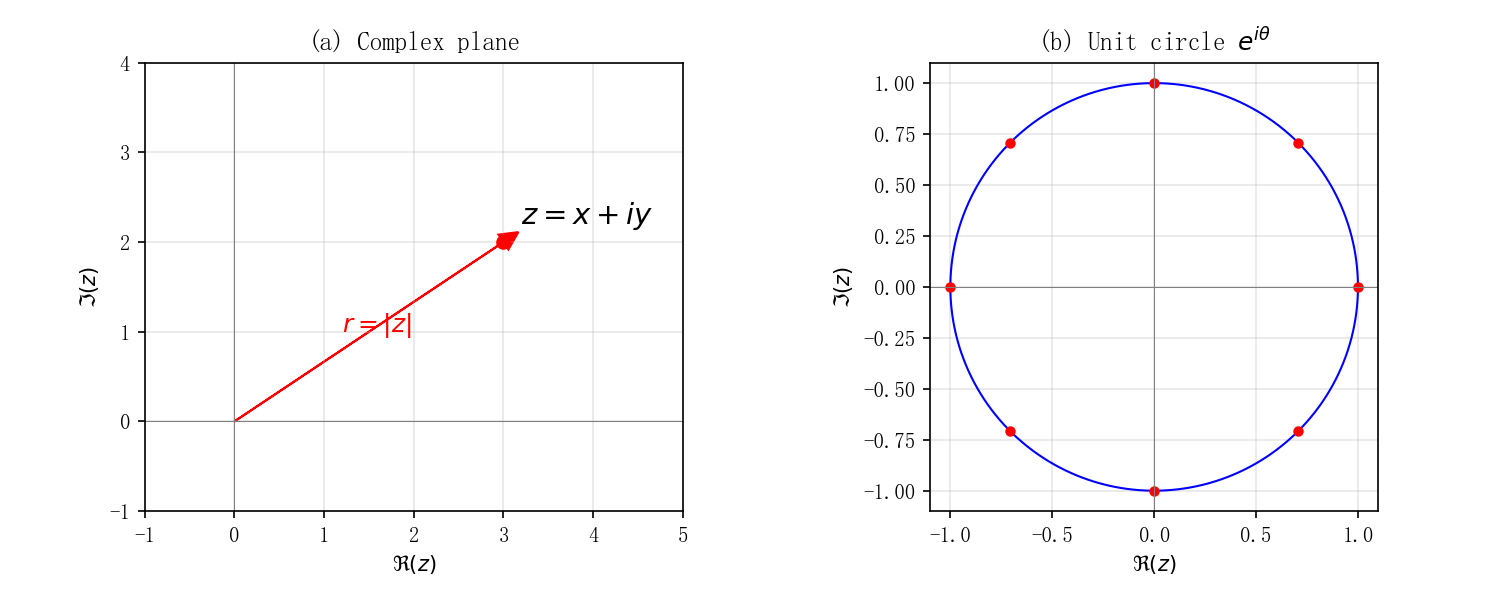
\includegraphics[width=0.75\textwidth]{figures/fig2_1_complex_plane.png}
\caption{左：复平面中 $z=x+iy$ 的矢量表示。右：单位圆 $e^{i\theta}$ 上的 8 个等分点。注意旋转 $\pi/4$ 对应乘以 $e^{i\pi/4}$。}
\label{fig:complex_plane}
\end{figure}

\subsection{复数的代数运算}

设 $z_1 = x_1 + \mathrm{i}y_1$, $z_2 = x_2 + \mathrm{i}y_2$：

\begin{align*}
\text{加法：}\quad &z_1 + z_2 = (x_1+x_2) + \mathrm{i}(y_1+y_2),\\
\text{乘法：}\quad &z_1 z_2 = (x_1 x_2 - y_1 y_2) + \mathrm{i}(x_1 y_2 + x_2 y_1),\\
\text{共轭：}\quad &\bar{z} = x - \mathrm{i}y,\quad z\bar{z} = |z|^2 = x^2 + y^2,\\
\text{除法：}\quad &\frac{z_1}{z_2} = \frac{z_1\bar{z_2}}{|z_2|^2} = \frac{(x_1 x_2 + y_1 y_2) + \mathrm{i}(x_2 y_1 - x_1 y_2)}{x_2^2 + y_2^2}.
\end{align*}

乘法的极坐标形式尤为优雅：$z_1 z_2 = r_1 r_2 e^{\mathrm{i}(\theta_1 + \theta_2)}$——模长相乘，辐角相加。这意味着乘法 = 旋转 + 缩放。

\begin{example}[复数的基本运算]
设 $z_1 = 1 + 2\mathrm{i}$, $z_2 = 3 - \mathrm{i}$。计算：

\textbf{(1)} $z_1 + z_2 = (1+3) + \mathrm{i}(2-1) = 4 + \mathrm{i}$。

\textbf{(2)} $z_1 z_2 = (1\cdot3 - 2\cdot(-1)) + \mathrm{i}(1\cdot(-1) + 2\cdot3) = (3+2) + \mathrm{i}(-1+6) = 5 + 5\mathrm{i}$。

用极坐标验证：$z_1 = \sqrt{5}e^{\mathrm{i}\arctan 2}$, $z_2 = \sqrt{10}e^{-\mathrm{i}\arctan(1/3)}$，乘积的模为 $\sqrt{50}=5\sqrt{2}$，辐角为 $\arctan 2 - \arctan(1/3) = \arctan(1)$（可以验证），所以确实 $5 + 5\mathrm{i}=5\sqrt{2}e^{\mathrm{i}\pi/4}$。

\textbf{(3)} $1/z_1 = \frac{1-2\mathrm{i}}{1^2+2^2} = \frac{1}{5} - \frac{2}{5}\mathrm{i}$。

\textbf{(4)} $|z_1| = \sqrt{1^2+2^2} = \sqrt{5}$, $|\bar{z}_1| = \sqrt{5}$, $\overline{z_1+z_2} = 4 - \mathrm{i}$。
\end{example}

\begin{insight}[相量法的物理核心]
交流电路中的正弦激励 $V(t) = V_0\cos(\omega t + \phi)$ 可以看作复相量 $V_0 e^{\mathrm{i}(\omega t+\phi)}$ 的实部。微分和积分运算变为：
\begin{align}
\frac{\dd}{\dd t} e^{\mathrm{i}\omega t} &= \mathrm{i}\omega e^{\mathrm{i}\omega t},\\
\int e^{\mathrm{i}\omega t}\,\dd t &= \frac{1}{\mathrm{i}\omega} e^{\mathrm{i}\omega t}.
\end{align}
于是 $RLC$ 串联电路的微分方程
\begin{equation}
L\frac{\dd I}{\dd t} + RI + \frac{1}{C}\int I\,\dd t = V(t)
\end{equation}
变为复数代数方程
\begin{equation}
\left(\mathrm{i}\omega L + R + \frac{1}{\mathrm{i}\omega C}\right)\tilde{I} = \tilde{V},
\end{equation}
其中括号内正是复阻抗 $Z$。这就是相量法——将时域微积分转化为频域代数运算，极大简化了线性电路分析。
\end{insight}

\subsection{复数的几何意义}

复数的乘法有重要的几何解释：

\begin{itemize}
\item 乘以 $re^{\mathrm{i}\theta}$ = 缩放 $r$ 倍 + 逆时针旋转 $\theta$ 角。
\item 乘以 $\mathrm{i}$ = 逆时针旋转 $90^\circ$（因为 $\mathrm{i} = e^{\mathrm{i}\pi/2}$）。
\item 乘以 $-1$ = 旋转 $180^\circ$。
\end{itemize}

\begin{example}[几何意义的可视化]
在复平面上画出下列变换：

\textbf{(1)} $z \to \mathrm{i}z$：点 $(x,y)$ 被映射到 $(-y,x)$，即绕原点逆时针旋转 $90^\circ$。

\textbf{(2)} $z \to z^2$：模变为平方，辐角加倍。单位圆上的点 $e^{\mathrm{i}\theta}$ 变为 $e^{2\mathrm{i}\theta}$——这意味着单位圆上的点被"拉伸"到两倍角速度。它在物理中的一个应用是倍频器。

\textbf{(3)} $z \to 1/z$：模取倒数，辐角变号。这是反演变换，将单位圆内的点映射到外部，反之亦然。
\end{example}

\subsection{复数的乘幂与单位根}

棣莫弗公式：
\begin{equation}
(re^{\mathrm{i}\theta})^n = r^n e^{\mathrm{i}n\theta},
\quad
z^{1/n} = r^{1/n} e^{\mathrm{i}(\theta+2\pi k)/n},\; k=0,1,\dots,n-1.
\end{equation}

单位根 $z^n = 1$ 的 $n$ 个解均匀分布在单位圆上：
\begin{equation}
\omega_k = e^{2\pi\mathrm{i}k/n},\quad k=0,1,\dots,n-1.
\end{equation}

\begin{example}[完整算例：三次单位根]
求 $z^3 = 1$ 的所有解。
\begin{align*}
z_0 &= e^{0} = 1,\\
z_1 &= e^{2\pi\mathrm{i}/3} = -\frac12 + \mathrm{i}\frac{\sqrt3}{2},\\
z_2 &= e^{4\pi\mathrm{i}/3} = -\frac12 - \mathrm{i}\frac{\sqrt3}{2}.
\end{align*}
三个解在复平面上构成等边三角形。验证：$1 + z_1 + z_2 = 0$。
\end{example}

\begin{example}[四次单位根与离散傅里叶变换]
$z^4 = 1$ 的四个解为 $1,\mathrm{i},-1,-\mathrm{i}$。将它们记为 $\omega_0=1,\omega_1=\mathrm{i},\omega_2=-1,\omega_3=-\mathrm{i}$。

这四个根构成了 $4\times4$ 傅里叶矩阵的基础：
\begin{equation}
F_{jk} = \frac{1}{\sqrt{4}}\omega_4^{-jk},\quad j,k=0,1,2,3.
\end{equation}
这是 DFT（离散傅里叶变换）在 $N=4$ 时的特例，将在第 3 章中详细讨论。
\end{example}

\subsection{复数的物理应用：交流电路中的复阻抗}

\begin{example}[完整算例：RC 电路的低通滤波特性]
考虑一个串联 RC 电路，电阻 $R$，电容 $C$，输入电压 $V_{\text{in}}(t) = V_0\cos(\omega t)$。

\textbf{步骤 1：写出复阻抗。}
$Z_R = R$, $Z_C = 1/(\mathrm{i}\omega C) = -\mathrm{i}/(\omega C)$。
总阻抗 $Z = R + 1/(\mathrm{i}\omega C) = R - \mathrm{i}/(\omega C)$。

\textbf{步骤 2：计算复电流。}
$\tilde{I} = \frac{\tilde{V}_{\text{in}}}{Z} = \frac{V_0}{R - \mathrm{i}/(\omega C)}$。

\textbf{步骤 3：输出电压（电容两端）。}
\begin{align*}
\tilde{V}_{\text{out}} &= \tilde{I} \cdot \frac{1}{\mathrm{i}\omega C}
= V_0 \frac{1/(\mathrm{i}\omega C)}{R + 1/(\mathrm{i}\omega C)} \\
&= V_0 \frac{1}{1 + \mathrm{i}\omega RC}.
\end{align*}

\textbf{步骤 4：传递函数。}
\begin{equation}
H(\omega) = \frac{\tilde{V}_{\text{out}}}{\tilde{V}_{\text{in}}}
= \frac{1}{1 + \mathrm{i}\omega RC}.
\end{equation}

\textbf{步骤 5：幅频和相频特性。}
\begin{align}
|H(\omega)| &= \frac{1}{\sqrt{1 + (\omega RC)^2}},\\
\angle H(\omega) &= -\arctan(\omega RC).
\end{align}

\textbf{物理意义：} 当 $\omega \ll 1/(RC)$ 时，$|H|\approx 1$——低频信号通过。当 $\omega \gg 1/(RC)$ 时，$|H|\sim 1/(\omega RC) \to 0$——高频信号被衰减。这正是\textbf{低通滤波器}。截止频率 $\omega_c = 1/(RC)$。
\end{example}

\section{解析函数与柯西-黎曼方程}
\label{sec:cauchy_riemann}

\subsection*{动机：从实函数到复函数的飞跃}

实函数的可导要求"左导数 = 右导数"，而复函数的可导要求"来自任何方向的导数都相等"。这看似是一个更严格的条件，但它带来的回报是惊人的——解析函数具有实函数不具备的"刚性"：一旦在一个小区域解析，全局性质就被完全确定。

\subsection{复变函数的导数}

定义：
\begin{equation}
f'(z_0) = \lim_{\Delta z\to 0}\frac{f(z_0+\Delta z) - f(z_0)}{\Delta z},
\end{equation}
其中 $\Delta z = \Delta x + \mathrm{i}\Delta y$ 可以从任何方向趋近于 $0$。如果极限存在且与路径无关，则称 $f$ 在 $z_0$ \textbf{可导}。

这个"与路径无关"的要求极为苛刻——它迫使复变函数的实部和虚部之间必须满足一组偏微分方程。

\subsection{柯西-黎曼方程}

设 $f(z) = u(x,y) + \mathrm{i}\,v(x,y)$。从实轴方向 ($\Delta y=0$) 和虚轴方向 ($\Delta x=0$) 分别求导并令相等：
\begin{align}
\text{实轴方向：}\quad f'(z) &= \frac{\partial u}{\partial x} + \mathrm{i}\frac{\partial v}{\partial x},\\
\text{虚轴方向：}\quad f'(z) &= \frac{1}{\mathrm{i}}\frac{\partial u}{\partial y} + \frac{\partial v}{\partial y}
= \frac{\partial v}{\partial y} - \mathrm{i}\frac{\partial u}{\partial y}.
\end{align}

令实部和虚部分别相等，得到 \textbf{柯西-黎曼方程}：
\begin{equation}
\boxed{\;\frac{\partial u}{\partial x} = \frac{\partial v}{\partial y},\qquad
\frac{\partial u}{\partial y} = -\frac{\partial v}{\partial x}\;}.
\label{eq:cauchy_riemann}
\end{equation}

它们是 $f(z)$ 可导的充要条件（在 $u,v$ 连续可微的前提下）。

\begin{theorem}
$f(z)$ 在区域 $D$ 内解析（全纯）当且仅当 $u,v$ 在 $D$ 内连续可微且满足柯西-黎曼方程。
\end{theorem}

\textbf{一个重要推论：} 解析函数 $f(z)$ 的导数可由下式给出：
\begin{equation}
f'(z) = \frac{\partial u}{\partial x} + \mathrm{i}\frac{\partial v}{\partial x}
= \frac{\partial v}{\partial y} - \mathrm{i}\frac{\partial u}{\partial y}.
\label{eq:complex_derivative}
\end{equation}

\begin{example}[验证柯西-黎曼方程：$f(z)=z^2$]
$f(z) = (x+\mathrm{i}y)^2 = (x^2-y^2) + \mathrm{i}(2xy)$。
所以 $u(x,y)=x^2-y^2$，$v(x,y)=2xy$。

柯西-黎曼验证：
\begin{align*}
\frac{\partial u}{\partial x} &= 2x,\quad \frac{\partial v}{\partial y} = 2x \;\Rightarrow\; \text{相等}\\
\frac{\partial u}{\partial y} &= -2y,\quad \frac{\partial v}{\partial x} = 2y \;\Rightarrow\; \frac{\partial u}{\partial y} = -\frac{\partial v}{\partial x}
\end{align*}
成立！导数为 $f'(z) = 2x + \mathrm{i}2y = 2z$，这正是我们预期的。
\end{example}

\begin{example}[反例：$f(z)=\bar{z}$ 处处不可导]
$f(z) = x - \mathrm{i}y$，$u=x$，$v=-y$。

柯西-黎曼检验：
\begin{align*}
\frac{\partial u}{\partial x} = 1,\quad \frac{\partial v}{\partial y} = -1 \;\Rightarrow\; \text{不相等！}
\end{align*}
因此 $f(z)=\bar{z}$ 在任何点都不可导。这就是复共轭不是解析函数的严格证据。
\end{example}

\begin{example}[指数函数的解析性验证]
$f(z) = e^z = e^x(\cos y + \mathrm{i}\sin y)$，所以 $u=e^x\cos y$, $v=e^x\sin y$。

\begin{align*}
\frac{\partial u}{\partial x} &= e^x\cos y,\quad \frac{\partial v}{\partial y} = e^x\cos y,\\
\frac{\partial u}{\partial y} &= -e^x\sin y,\quad \frac{\partial v}{\partial x} = e^x\sin y.
\end{align*}
满足 C-R 方程！导数为 $f'(z) = e^x\cos y + \mathrm{i}e^x\sin y = e^z$。这说明指数函数在整个复平面上解析。
\end{example}

\subsection{拉普拉斯方程与调和函数}

对柯西-黎曼方程交叉求导：
\begin{align}
\frac{\partial^2 u}{\partial x^2} &= \frac{\partial}{\partial x}\frac{\partial v}{\partial y}
= \frac{\partial}{\partial y}\frac{\partial v}{\partial x}
= -\frac{\partial^2 u}{\partial y^2},\\
\therefore\quad \nabla^2 u &= 0,\qquad \nabla^2 v = 0.
\end{align}

\textbf{解析函数的实部和虚部都是调和函数}（满足拉普拉斯方程）。这样的实-虚对称为\textbf{共轭调和函数}。

\begin{insight}[二维物理场的天然语言]
二维静电场（无源区）满足 $\nabla^2\phi = 0$，二维不可压缩无旋流场的流函数和速度势也满足拉普拉斯方程。解析函数同时给出了势函数 $u$ 和流函数 $v$：
\begin{itemize}
\item 等势线：$u(x,y) = \text{常数}$
\item 场/流线：$v(x,y) = \text{常数}$
\end{itemize}
而且两条曲线处处正交（因为柯西-黎曼方程意味着 $\nabla u\cdot\nabla v = 0$）！一个简单的例子：$f(z) = z^2 = (x^2-y^2) + \mathrm{i}(2xy)$ 描述了角域中的电场分布。等势线 $x^2-y^2=C$ 是双曲线，流线 $2xy=C$ 也是双曲线但与之正交。
\end{insight}

\begin{example}[由实部求解析函数]
已知 $u(x,y) = x^3 - 3xy^2$，求 $v(x,y)$ 使得 $f=u+\mathrm{i}v$ 解析。

\textbf{步骤 1：验证 $u$ 是调和函数。}
\begin{align*}
\frac{\partial^2 u}{\partial x^2} &= 6x,\quad
\frac{\partial^2 u}{\partial y^2} = -6x,\\
\nabla^2 u &= 6x + (-6x) = 0. \quad\text{成立。}
\end{align*}

\textbf{步骤 2：利用 C-R 方程求 $v$。}
\begin{align*}
\frac{\partial v}{\partial y} &= \frac{\partial u}{\partial x} = 3x^2 - 3y^2,\\
\frac{\partial v}{\partial x} &= -\frac{\partial u}{\partial y} = 6xy.
\end{align*}

\textbf{步骤 3：积分求 $v$。}
由第一式：$v = \int (3x^2 - 3y^2)\,\dd y = 3x^2 y - y^3 + \phi(x)$。
由第二式：$\frac{\partial v}{\partial x} = 6xy + \phi'(x) = 6xy$，所以 $\phi'(x)=0$，$\phi(x)=C$。

取 $C=0$，得 $v = 3x^2 y - y^3$。

\textbf{步骤 4：写出 $f(z)$。}
$f(z) = (x^3-3xy^2) + \mathrm{i}(3x^2y - y^3) = (x+\mathrm{i}y)^3 = z^3$。
完美！
\end{example}

\subsection{初等解析函数}

\textbf{多项式：} $f(z) = a_n z^n + \cdots + a_0$，在全平面解析（整函数）。

\textbf{有理函数：} $f(z) = P(z)/Q(z)$，在 $Q(z)\neq0$ 处解析。$Q(z)=0$ 的点是奇点（极点）。

\textbf{指数函数：}
\begin{equation}
e^z = e^x(\cos y + \mathrm{i}\sin y),\quad
(e^z)' = e^z.
\end{equation}
指数函数没有零点（$|e^z| = e^x > 0$），且 $e^{z+2\pi\mathrm{i}} = e^z$——指数函数以 $2\pi\mathrm{i}$ 为周期。这一点与实指数函数有本质不同。

\textbf{三角函数：}
\begin{equation}
\sin z = \frac{e^{\mathrm{i}z} - e^{-\mathrm{i}z}}{2\mathrm{i}},\quad
\cos z = \frac{e^{\mathrm{i}z} + e^{-\mathrm{i}z}}{2}.
\end{equation}
当 $z=\mathrm{i}y$ 为纯虚数时，$\sin(\mathrm{i}y) = \mathrm{i}\sinh y$——三角函数和双曲函数在复域中统一了。复三角函数不再有界：$|\sin(\mathrm{i}y)| = |\sinh y|$ 可以趋于无穷。

\textbf{双曲函数：}
\begin{equation}
\sinh z = \frac{e^z - e^{-z}}{2},\quad
\cosh z = \frac{e^z + e^{-z}}{2}.
\end{equation}
关系：$\sin(\mathrm{i}z) = \mathrm{i}\sinh z$, $\cos(\mathrm{i}z) = \cosh z$。

\textbf{对数函数：}
\begin{equation}
\ln z = \ln|z| + \mathrm{i}\arg z.
\end{equation}
由于辐角的多值性，$\ln z$ 是多值函数。指定主值 $\Arg z \in (-\pi,\pi]$ 得到主值分支。

\textbf{一般幂函数：}
\begin{equation}
z^\alpha = e^{\alpha\ln z},\quad \alpha\in\mathbb{C}.
\end{equation}
由于 $\ln z$ 的多值性，$z^\alpha$ 一般也是多值的。当 $\alpha$ 为整数时退化为单值。这解释了为什么 $z^{1/2}$ 有两个值、$z^{1/3}$ 有三个值。

\section{多值函数、黎曼曲面与支点}
\label{sec:multivalued}

\subsection*{动机：为什么有些函数会有多个值？}

你可能在实分析中习惯了 $\sqrt{4}=2$ 的唯一性。但在复平面上 $\sqrt{4}=?$ 走一圈回到原点后，$\sqrt{z}$ 自动变成了 $-\sqrt{z}$。这不是混淆，而是一个更深层结构的信号——黎曼曲面。

\subsection{多值性的来源}

复数开方和对数产生多值性，根本原因在于辐角 $\arg z$ 的多值性：绕原点一周，$\arg z$ 增加 $2\pi$。

对于 $f(z) = z^{1/2}$，$z = re^{\mathrm{i}\theta}$ 的平方根为：
\begin{equation}
\sqrt{z} = \sqrt{r}\,e^{\mathrm{i}\theta/2}
\quad\text{或}\quad \sqrt{r}\,e^{\mathrm{i}(\theta+2\pi)/2} = -\sqrt{r}\,e^{\mathrm{i}\theta/2}.
\end{equation}

\textbf{支点 (branch point)} 是多值函数的关键点——绕该点一周函数值发生变化。$z=0$ 是 $\sqrt{z}$ 和 $\ln z$ 的支点，无穷远点也是。

\textbf{割线 (branch cut)} 用来将多值函数限制为单值分支。例如，对 $\sqrt{z}$ 取负实轴为割线，规定 $\theta \in (-\pi,\pi]$ 即得主值分支。

\begin{example}[多值性的数值体验]
计算 $\sqrt{4}$ 在复平面的意义：
\begin{align*}
4 &= 4e^{\mathrm{i}\cdot 0} \;\Rightarrow\; \sqrt{4} = 2e^{\mathrm{i}0} = 2,\\
4 &= 4e^{\mathrm{i}\cdot 2\pi} \;\Rightarrow\; \sqrt{4} = 2e^{\mathrm{i}\pi} = -2.
\end{align*}
两个结果都满足 $(\pm2)^2 = 4$。在实分析中我们约定取正根，但复分析要求我们正视这种多值性。
\end{example}

\subsection{黎曼曲面的直观}

黎曼曲面的想法是：不是限制多值函数的定义域，而是为多值函数的每一个"分支"分配一个独立的复平面层，然后将这些层在割线处粘合。这样，多值函数在新的"分层"空间上变成了单值函数。

例如，$\sqrt{z}$ 的黎曼曲面由两层组成：
\begin{itemize}
\item 第一层：$\theta \in (-\pi,\pi]$，$\sqrt{z} = \sqrt{r}e^{\mathrm{i}\theta/2}$。
\item 第二层：$\theta \in (\pi,3\pi]$，$\sqrt{z} = \sqrt{r}e^{\mathrm{i}\theta/2} = -\sqrt{r}e^{\mathrm{i}(\theta-2\pi)/2}$。
\end{itemize}
在割线（负实轴）处，第一层的下岸连接到第二层的上岸，反之亦然。因此，绕原点两周后回到第一层——$\sqrt{z}$ 在两层黎曼曲面上是单值的。

对于 $\ln z$，其黎曼曲面有无限多层——每一层的虚部相差 $2\pi$。这反映了 $\ln z$ 的无限多值性。

\begin{example}[物理中的支点：色散关系]
在等离子体物理和光学中，介电函数 $\varepsilon(\omega)$ 在复 $\omega$ 平面上具有支点割线结构。解析性质（Kramers-Kronig 关系）保证了因果性——$\varepsilon(\omega)$ 的实部和虚部通过希尔伯特变换相联系。这是多值函数理论在现代物理中的精彩应用。
\end{example}

\begin{example}[割线选择的物理后果：$\sqrt{z^2-1}$]
在空气动力学中，Joukowski 映射 $w = z + 1/z$ 涉及函数 $\sqrt{z^2-1}$。割线的选择决定了物理平面上流动的拓扑结构：选择连接 $z=1$ 和 $z=-1$ 之间的线段作为割线，对应的是绕薄翼型的流动；选择通过无穷远点的割线则对应不同的流动拓扑。割线的位置不是任意的——它由物理边界条件决定。
\end{example}

\section{复变积分}
\label{sec:complex_integration}

\subsection*{动机：为什么要沿曲线积分？}

复变函数沿曲线的积分是通往留数定理的必经之路。与实变积分不同，复积分的结果不仅依赖于起点和终点，还依赖于路径是否绕过了奇点。这种"路径依赖"恰恰是留数定理力量的来源。

\subsection{复积分定义与基本性质}

沿复平面上有向曲线 $C$ 的积分：
\begin{equation}
\int_C f(z)\,\dd z = \int_C (u+\mathrm{i}v)(\dd x + \mathrm{i}\dd y)
= \int_C (u\dd x - v\dd y) + \mathrm{i}\int_C (v\dd x + u\dd y).
\end{equation}

这表明复积分本质上是一对实线积分。如果 $C$ 由参数方程 $z(t) = x(t) + \mathrm{i}y(t)$, $t\in[a,b]$ 给出，则
\begin{equation}
\int_C f(z)\,\dd z = \int_a^b f(z(t))\,z'(t)\,\dd t.
\end{equation}

\textbf{基本性质：}
\begin{itemize}
\item 线性：$\int_C (\alpha f + \beta g)\,\dd z = \alpha\int_C f\,\dd z + \beta\int_C g\,\dd z$。
\item 方向反转：$\int_{-C} f\,\dd z = -\int_C f\,\dd z$（$-C$ 表示反向路径）。
\item 路径拼接：若 $C = C_1 + C_2$（首尾相接），则 $\int_C = \int_{C_1} + \int_{C_2}$。
\end{itemize}

\textbf{ML 不等式（估值引理）：} 若在曲线 $C$ 上 $|f(z)| \leq M$，且 $C$ 的长度为 $L$，则
\begin{equation}
\left|\int_C f(z)\,\dd z\right| \leq M L.
\label{eq:ml_inequality}
\end{equation}
这个引理在围道积分中用来证明某些部分（如半圆）的贡献在半径趋于无穷时为零。

\begin{example}[完整算例：沿直线段的复积分]
计算 $\displaystyle\int_C z\,\dd z$，其中 $C$ 是从 $0$ 到 $1+\mathrm{i}$ 的直线段。

\textbf{步骤 1：参数化路径。}
$z(t) = (1+\mathrm{i})t$，$t\in[0,1]$，$\dd z = (1+\mathrm{i})\dd t$。

\textbf{步骤 2：代入被积函数。}
$\displaystyle\int_C z\,\dd z = \int_0^1 (1+\mathrm{i})t \cdot (1+\mathrm{i})\dd t
= (1+\mathrm{i})^2\int_0^1 t\,\dd t$。

\textbf{步骤 3：计算。}
$(1+\mathrm{i})^2 = 2\mathrm{i}$，$\int_0^1 t\,\dd t = \frac12$。
所以 $\int_C z\,\dd z = 2\mathrm{i} \cdot \frac12 = \mathrm{i}$。

\textbf{验证：} $z$ 在全平面解析，其原函数为 $z^2/2$。
$\int_C z\,\dd z = \frac12 z^2\big|_{z=0}^{z=1+\mathrm{i}} = \frac12(1+\mathrm{i})^2 = \frac12(2\mathrm{i}) = \mathrm{i}$。一致。
\end{example}

\begin{example}[沿不同路径的积分：$\int 1/z\,\dd z$]
设 $C$ 是绕单位圆的逆时针路径，$z = e^{\mathrm{i}\theta}$, $\theta\in[0,2\pi]$。

\begin{align*}
\oint_{|z|=1} \frac{1}{z}\,\dd z
&= \int_0^{2\pi} \frac{1}{e^{\mathrm{i}\theta}} \cdot \mathrm{i}e^{\mathrm{i}\theta}\,\dd\theta
= \int_0^{2\pi} \mathrm{i}\,\dd\theta = 2\pi\mathrm{i}.
\end{align*}

这个结果极为重要——它不为零！注意 $f(z)=1/z$ 在 $z=0$ 处不解析（奇点位于圆内）。对解析函数，柯西积分定理将告诉我们闭合路径积分为零；而对有奇点的函数，结果正是留数的 $2\pi\mathrm{i}$ 倍。
\end{example}

\subsection{柯西积分定理}

\textbf{柯西积分定理：} 若 $f(z)$ 在单连通区域 $D$ 内解析，则 $f$ 沿 $D$ 内任意闭合路径的积分为零：
\begin{equation}
\oint_C f(z)\,\dd z = 0.
\label{eq:cauchy_integral_theorem}
\end{equation}

\textbf{证明思路：} 由柯西-黎曼方程和格林定理，
\begin{align}
\oint_C (u\dd x - v\dd y) &= -\iint_S \left(\frac{\partial v}{\partial x} + \frac{\partial u}{\partial y}\right)\dd x\dd y = 0,\\
\oint_C (v\dd x + u\dd y) &= \iint_S \left(\frac{\partial u}{\partial x} - \frac{\partial v}{\partial y}\right)\dd x\dd y = 0,
\end{align}
其中 $S$ 是 $C$ 所围区域。两个被积函数均为零正是柯西-黎曼方程的结果。

\textbf{重要推论：} 解析函数的积分与路径无关，只取决于起点和终点。这允许我们自由变形积分路径——只要不穿过非解析区域。

\textbf{推广——多连通区域的柯西定理：} 若 $f(z)$ 在由外曲线 $C_0$ 和内曲线 $C_1,C_2,\dots,C_n$ 围成的多连通区域内解析，则
\begin{equation}
\oint_{C_0} f\,\dd z = \sum_{k=1}^n \oint_{C_k} f\,\dd z,
\end{equation}
其中所有路径取相同的定向（如逆时针）。这个性质在围道变形中极为有用——我们可以将围绕多个奇点的复杂围道变形为围绕每个奇点的小圆周之和。

\subsection{柯西积分公式}

设 $f(z)$ 在简单闭曲线 $C$ 内部及边界上解析，$z_0$ 为 $C$ 内任意一点，则
\begin{equation}
\boxed{\;f(z_0) = \frac{1}{2\pi\mathrm{i}}\oint_C \frac{f(z)}{z - z_0}\,\dd z\;}.
\label{eq:cauchy_integral_formula}
\end{equation}

这一公式的深刻之处在于：\textbf{解析函数在区域内任意一点的值完全由其在边界上的值决定}。这是解析函数"刚性"的体现——全局决定局部。

\textbf{高阶导数公式：}
\begin{equation}
f^{(n)}(z_0) = \frac{n!}{2\pi\mathrm{i}}\oint_C \frac{f(z)}{(z - z_0)^{n+1}}\,\dd z.
\label{eq:cauchy_derivative}
\end{equation}

\begin{example}[完整算例：柯西积分公式的应用]
计算 $\displaystyle\oint_{|z|=2} \frac{e^z}{z-1}\,\dd z$。

\textbf{识别：} $f(z)=e^z$ 在全平面解析，$z_0=1$ 位于圆 $|z|=2$ 内部。
由柯西积分公式：
\begin{equation}
\oint_{|z|=2} \frac{e^z}{z-1}\,\dd z = 2\pi\mathrm{i}\, e^1 = 2\pi\mathrm{i}\, e.
\end{equation}
不需要做任何积分计算！

\textbf{变体：} 如果是 $\oint_{|z|=0.5} \frac{e^z}{z-1}\,\dd z$，奇点 $z=1$ 不在圆内，由柯西积分定理，积分为零。
\end{example}

\begin{example}[高阶导数公式的应用]
计算 $\displaystyle\oint_{|z|=2} \frac{e^z}{(z-1)^3}\,\dd z$。

由高阶导数公式，$n=2$，$z_0=1$：
\begin{align*}
\oint_{|z|=2} \frac{e^z}{(z-1)^3}\,\dd z
&= \frac{2\pi\mathrm{i}}{2!} f''(1),\quad f(z)=e^z,\; f''(z)=e^z,\\
&= \pi\mathrm{i}\, e.
\end{align*}
\end{example}

\begin{insight}[柯西积分公式的物理解读]
二维静电场中，$f(z) = \phi(x,y) + \mathrm{i}\psi(x,y)$ 是解析函数（势函数 + 流函数）。柯西积分公式表明：\textbf{区域边界的电场分布唯一确定了内部任意点的电势}。这正是拉普拉斯方程边值问题解的唯一性和稳定性的数学根源。
\end{insight}

\subsection{柯西积分公式的推广：泊松积分公式}

柯西积分公式取实部可以导出一个极为重要的结果：对于上半平面 $\Im z > 0$ 内的解析函数，其边界值（实轴上的值）决定了内部的值。

设 $f(z)$ 在上半平面解析且在实轴上足够快地衰减，则
\begin{equation}
f(z) = \frac{1}{\pi\mathrm{i}}\int_{-\infty}^{\infty} \frac{f(t)}{t-z}\,\dd t,\quad \Im z > 0.
\end{equation}

取实部得到\textbf{泊松积分公式}：
\begin{equation}
u(x,y) = \frac{y}{\pi}\int_{-\infty}^{\infty} \frac{u(t,0)}{(t-x)^2 + y^2}\,\dd t.
\end{equation}
这在势论中意味着：上半平面的调和函数完全由实轴上的边界值决定。这将在 \S2.8 的 Kramers-Kronig 关系中再次出现。

\section{留数定理}
\label{sec:residue}

\subsection*{动机：从困难到简单}

计算 $\int_{-\infty}^{\infty} \frac{\cos x}{1+x^2}\,\dd x$ 用实分析技巧可以算，但很啰嗦。留数定理把它变成了一个极点的留数计算——两步写完。这就是复变函数最实用的地方。

% 围道积分示意图
\begin{figure}[H]
\centering
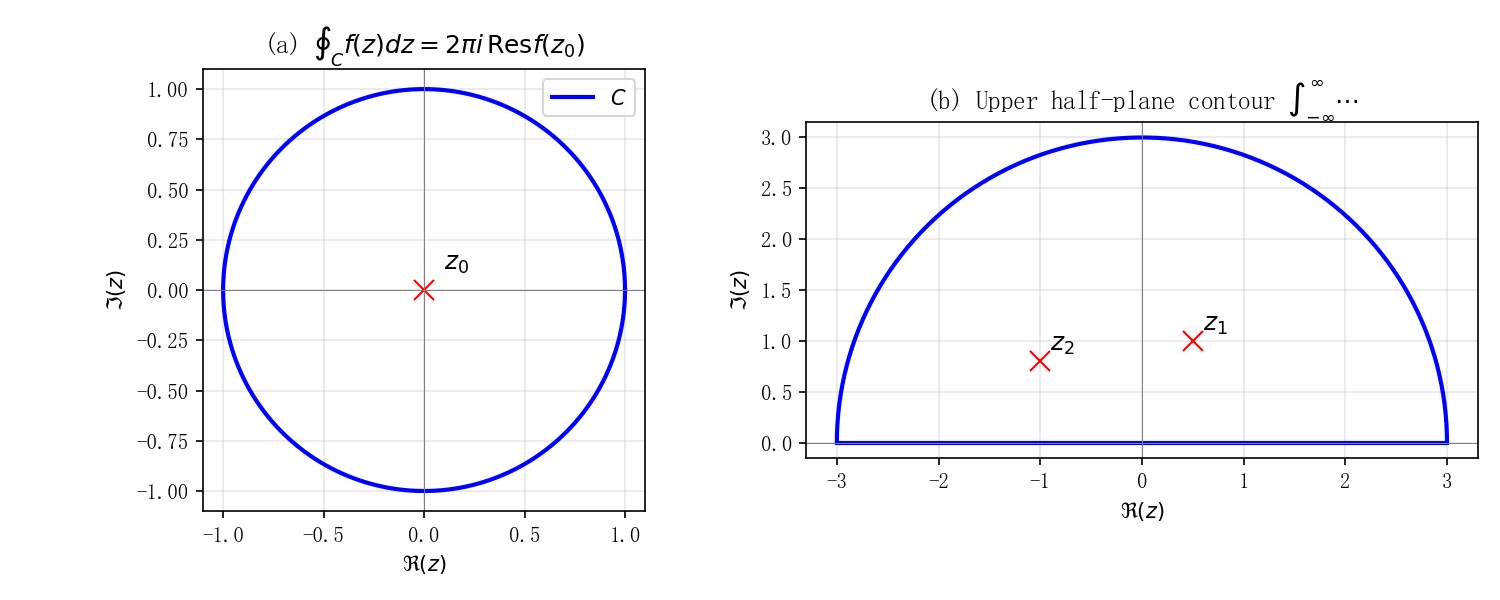
\includegraphics[width=0.75\textwidth]{figures/fig2_2_contour.png}
\caption{左：绕孤立奇点 $z_0$ 的简单围道。右：计算 $\int_{-\infty}^{\infty} f(x)\,\dd x$ 的上半平面围道，$z_1$ 和 $z_2$ 是上半平面的极点。}
\label{fig:contour}
\end{figure}

\subsection{孤立奇点的分类}

\textbf{可去奇点：} $\lim_{z\to z_0}f(z)$ 存在有限。例如 $z=0$ 是 $\sin z/z$ 的可去奇点（因为极限为 $1$）。通过重新定义 $f(0)=1$，奇点可以被"消除"。

\textbf{极点：} $\lim_{z\to z_0}|f(z)| = \infty$。$n$ 阶极点意味着 $(z-z_0)^n f(z)$ 在 $z_0$ 解析且非零。例如 $f(z)=1/(z-1)^2$ 在 $z=1$ 处有二阶极点。

\textbf{本性奇点：} 极限不存在也不为无穷。例如 $z=0$ 是 $e^{1/z}$ 的本性奇点。在本性奇点的任意邻域内，函数可以取到任意复值（Casorati-Weierstrass 定理）。

\begin{example}[奇点分类练习]
对下列函数分类其奇点：

\textbf{(1)} $f(z) = \frac{z}{(z-1)(z+2)}$：$z=1$ 和 $z=-2$ 都是一阶极点。

\textbf{(2)} $f(z) = \frac{\sin z}{z^3}$：$z=0$。展开 $\sin z = z - z^3/3! + z^5/5! - \cdots$，所以 $f(z) = 1/z^2 - 1/6 + \cdots$，这是一个二阶极点。

\textbf{(3)} $f(z) = e^{1/z}$：$z=0$ 是本性奇点。洛朗展开为 $\sum_{n=0}^{\infty} 1/(n! z^n)$，负幂项无限多。

\textbf{(4)} $f(z) = \frac{z^2-1}{z-1}$：化简为 $z+1$（$z\neq1$），所以 $z=1$ 是可去奇点。
\end{example}

\subsection{洛朗展开}

在奇点 $z_0$ 附近，$f(z)$ 可以展开为洛朗级数：
\begin{equation}
f(z) = \sum_{n=-\infty}^{\infty} a_n (z-z_0)^n,
\end{equation}
其中
\begin{equation}
a_n = \frac{1}{2\pi\mathrm{i}}\oint_C \frac{f(z)}{(z-z_0)^{n+1}}\,\dd z.
\end{equation}

洛朗级数是泰勒级数的推广——它允许负幂项的存在。负幂项的存在与否直接对应奇点的类型：
\begin{itemize}
\item 无负幂项 $\to$ 可去奇点（实际上就是泰勒级数）。
\item 有限多项负幂 $\to$ 极点（最高负幂指数 $m$ 就是极点的阶）。
\item 无限多项负幂 $\to$ 本性奇点。
\end{itemize}

\textbf{留数} 就是 $a_{-1}$，即 $(z-z_0)^{-1}$ 项的系数：
\begin{equation}
\mathop{\mathrm{Res}}_{z=z_0} f(z) = a_{-1}
= \frac{1}{2\pi\mathrm{i}}\oint_{C_0} f(z)\,\dd z.
\label{eq:residue_def}
\end{equation}

\textbf{极点留数的计算：} 对于一阶极点，
\begin{equation}
\mathop{\mathrm{Res}}_{z=z_0} f(z) = \lim_{z\to z_0} (z-z_0)f(z).
\end{equation}
对于 $m$ 阶极点，
\begin{equation}
\mathop{\mathrm{Res}}_{z=z_0} f(z)
= \frac{1}{(m-1)!}\lim_{z\to z_0}
\frac{\dd^{m-1}}{\dd z^{m-1}}\left[(z-z_0)^m f(z)\right].
\label{eq:residue_pole}
\end{equation}

\begin{example}[留数计算练习]
计算下列函数在指定点的留数。

\textbf{(1)} $f(z) = \frac{1}{z-1}$，$z_0=1$：一阶极点。
$\mathop{\mathrm{Res}}_{z=1} f(z) = \lim_{z\to 1} (z-1)\frac{1}{z-1} = 1$。

\textbf{(2)} $f(z) = \frac{1}{(z-1)^2}$，$z_0=1$：二阶极点。
由公式：$\mathop{\mathrm{Res}}_{z=1}\frac{1}{(z-1)^2} = \frac{1}{1!}\lim_{z\to1}\frac{\dd}{\dd z}\left[(z-1)^2\frac{1}{(z-1)^2}\right] = \lim_{z\to1}\frac{\dd}{\dd z}(1)=0$。
直接观察洛朗展开：$f(z) = (z-1)^{-2}$，没有 $(z-1)^{-1}$ 项，所以留数确实为 $0$。

\textbf{(3)} $f(z) = \frac{e^z}{z^2}$，$z_0=0$：二阶极点。
展开 $e^z = 1 + z + z^2/2 + \cdots$，所以 $f(z) = 1/z^2 + 1/z + 1/2 + \cdots$，留数为 $1$（$z^{-1}$ 的系数）。
用公式验证：$\mathop{\mathrm{Res}}_{z=0}\frac{e^z}{z^2} = \frac{1}{1!}\lim_{z\to0}\frac{\dd}{\dd z}(e^z) = e^0 = 1$。

\textbf{(4)} $f(z) = \frac{1}{z^2+1}$，$z_0=\mathrm{i}$：一阶极点。
$\mathop{\mathrm{Res}}_{z=\mathrm{i}}\frac{1}{z^2+1} = \lim_{z\to\mathrm{i}} (z-\mathrm{i})\frac{1}{(z-\mathrm{i})(z+\mathrm{i})} = \frac{1}{2\mathrm{i}}$。
\end{example}

\subsection{留数定理}

\textbf{留数定理：} 设 $f(z)$ 在简单闭曲线 $C$ 内部除有限个孤立奇点 $z_1,\dots,z_n$ 外处处解析，在 $C$ 上解析，则
\begin{equation}
\boxed{\;\oint_C f(z)\,\dd z = 2\pi\mathrm{i}\sum_{k=1}^n
\mathop{\mathrm{Res}}_{z=z_k} f(z)\;}.
\label{eq:residue_theorem}
\end{equation}

这是复变函数论中最强大的定理——它将围道积分化为留数求和。

\subsection{实积分的计算}

留数定理最重要的应用之一是计算各种类型的实积分。我们按类型逐一讨论。

\subsubsection{类型 I：$\int_{-\infty}^{\infty} R(x)\,\dd x$，$R(x)$ 是有理函数}

要求 $R(x)$ 的分母次数至少比分子次数高 2 次，且分母无实零点。

\begin{example}[完整算例：$\displaystyle\int_{-\infty}^{\infty} \frac{\dd x}{1+x^2}$]
\textbf{步骤 1：构造复变函数。}
$f(z) = \frac{1}{1+z^2} = \frac{1}{(z+\mathrm{i})(z-\mathrm{i})}$。
$f(z)$ 有奇点 $z=\pm\mathrm{i}$。

\textbf{步骤 2：选择围道。}
取上半平面的半圆围道 $C_R = [-R,R] \cup \Gamma_R$（$\Gamma_R$ 是半径为 $R$ 的上半圆）。
当 $R\to\infty$ 时，$\Gamma_R$ 上的积分趋于零（因为 $|f(z)|\sim 1/R^2$，由 ML 不等式知 $|\int_{\Gamma_R}| \leq \pi R / R^2 = \pi/R \to 0$）。

\textbf{步骤 3：确定围道内的奇点。}
上半平面内的奇点只有 $z=\mathrm{i}$（一阶极点）。

\textbf{步骤 4：计算留数。}
\begin{equation}
\mathop{\mathrm{Res}}_{z=\mathrm{i}} \frac{1}{1+z^2}
= \lim_{z\to\mathrm{i}} (z-\mathrm{i})\frac{1}{(z-\mathrm{i})(z+\mathrm{i})}
= \frac{1}{\mathrm{i}+\mathrm{i}} = \frac{1}{2\mathrm{i}}.
\end{equation}

\textbf{步骤 5：应用留数定理。}
\begin{align*}
\oint_{C_R} f(z)\,\dd z
&= \int_{-R}^{R} \frac{\dd x}{1+x^2} + \int_{\Gamma_R} \frac{\dd z}{1+z^2} \\
&= 2\pi\mathrm{i} \cdot \frac{1}{2\mathrm{i}} = \pi.
\end{align*}
取 $R\to\infty$：
\begin{equation}
\int_{-\infty}^{\infty} \frac{\dd x}{1+x^2} = \pi.
\end{equation}
\textbf{结果印证：} $\arctan x|_{-\infty}^{\infty} = \pi/2 - (-\pi/2) = \pi$。一致！
\end{example}

\subsubsection{类型 II：$\int_{-\infty}^{\infty} R(x) e^{\mathrm{i}ax}\,\dd x$（含三角函数的积分）}

对这类积分，Jordan 引理提供了半圆上积分趋于零的条件。

\textbf{Jordan 引理：} 若 $f(z)$ 在上半平面当 $|z|\to\infty$ 时一致趋于 $0$，则对 $a>0$，
\begin{equation}
\lim_{R\to\infty}\int_{\Gamma_R} f(z) e^{\mathrm{i}az}\,\dd z = 0,
\end{equation}
其中 $\Gamma_R$ 是上半圆 $|z|=R$, $\Im z \geq 0$。

\begin{example}[完整算例：$\displaystyle\int_{-\infty}^{\infty} \frac{\cos x}{x^2+1}\,\dd x$]
\textbf{步骤 1：构造复变函数。}
考虑 $\displaystyle I = \int_{-\infty}^{\infty} \frac{e^{\mathrm{i}x}}{x^2+1}\,\dd x$，
目标积分为 $\Re(I)$。

令 $f(z) = \frac{e^{\mathrm{i}z}}{z^2+1}$。

\textbf{步骤 2：围道和奇点。}
上半平面半圆围道。奇点 $z=\pm\mathrm{i}$。上半平面内只有 $z=\mathrm{i}$。

\textbf{步骤 3：计算留数（一阶极点）。}
\begin{align*}
\mathop{\mathrm{Res}}_{z=\mathrm{i}} \frac{e^{\mathrm{i}z}}{(z+\mathrm{i})(z-\mathrm{i})}
&= \lim_{z\to\mathrm{i}} (z-\mathrm{i})\frac{e^{\mathrm{i}z}}{(z+\mathrm{i})(z-\mathrm{i})}
= \frac{e^{\mathrm{i}\cdot\mathrm{i}}}{\mathrm{i}+\mathrm{i}}
= \frac{e^{-1}}{2\mathrm{i}}.
\end{align*}

\textbf{步骤 4：应用留数定理。}
由 Jordan 引理，半圆上的积分在 $R\to\infty$ 时为零。因此
\begin{equation}
I = \int_{-\infty}^{\infty} \frac{e^{\mathrm{i}x}}{x^2+1}\,\dd x
= 2\pi\mathrm{i} \cdot \frac{e^{-1}}{2\mathrm{i}} = \frac{\pi}{e}.
\end{equation}

\textbf{步骤 5：取实部。}
\begin{equation}
\boxed{\;\int_{-\infty}^{\infty} \frac{\cos x}{x^2+1}\,\dd x = \frac{\pi}{e}\;},
\qquad
\int_{-\infty}^{\infty} \frac{\sin x}{x^2+1}\,\dd x = 0 \text{（奇函数）}.
\end{equation}
\end{example}

\begin{example}[$\displaystyle\int_0^{\infty} \frac{\sin x}{x}\,\dd x = \frac{\pi}{2}$]
这是物理学中最重要的积分之一，出现在衍射理论、信号处理和量子力学中。

\textbf{构造：} 考虑 $f(z) = \frac{e^{\mathrm{i}z}}{z}$，并取如下围道：由实轴 $[-R,-\varepsilon]$、小半圆 $C_\varepsilon$（半径 $\varepsilon$，上半平面）、实轴 $[\varepsilon,R]$、大半圆 $\Gamma_R$（半径 $R$）组成。

由于 $\frac{e^{\mathrm{i}z}}{z}$ 在围道内解析（原点被小半圆避开），总积分为 $0$：
\begin{equation}
\int_{-R}^{-\varepsilon} \frac{e^{\mathrm{i}x}}{x}\,\dd x
+ \int_{C_\varepsilon} \frac{e^{\mathrm{i}z}}{z}\,\dd z
+ \int_{\varepsilon}^{R} \frac{e^{\mathrm{i}x}}{x}\,\dd x
+ \int_{\Gamma_R} \frac{e^{\mathrm{i}z}}{z}\,\dd z = 0.
\end{equation}

$R\to\infty$ 时，$\Gamma_R$ 上积分由 Jordan 引理趋于 $0$。
$\varepsilon\to0$ 时，小半圆上的积分 $= -\pi\mathrm{i}\,\mathop{\mathrm{Res}}_{z=0}\frac{e^{\mathrm{i}z}}{z} = -\pi\mathrm{i}\cdot 1 = -\pi\mathrm{i}$（负号因为顺时针方向）。

合并实轴上的积分：
\begin{equation}
\int_{-\infty}^{\infty} \frac{e^{\mathrm{i}x}}{x}\,\dd x = \pi\mathrm{i}.
\end{equation}

取虚部：
\begin{equation}
\int_{-\infty}^{\infty} \frac{\sin x}{x}\,\dd x = \pi,\quad
\int_{0}^{\infty} \frac{\sin x}{x}\,\dd x = \frac{\pi}{2}.
\end{equation}
\end{example}

\subsubsection{类型 III：$\int_0^{2\pi} R(\cos\theta,\sin\theta)\,\dd\theta$}

令 $z = e^{\mathrm{i}\theta}$，则 $\cos\theta = (z+z^{-1})/2$，$\sin\theta = (z-z^{-1})/(2\mathrm{i})$，$\dd\theta = \dd z/(\mathrm{i}z)$：
\begin{equation}
\int_0^{2\pi} R(\cos\theta,\sin\theta)\,\dd\theta
= \oint_{|z|=1} \frac{1}{\mathrm{i}z}R\left(\frac{z+z^{-1}}{2},
\frac{z-z^{-1}}{2\mathrm{i}}\right)\dd z.
\end{equation}

\begin{example}[$\displaystyle\int_0^{2\pi} \frac{\dd\theta}{a+\cos\theta}$, $a>1$]
令 $z=e^{\mathrm{i}\theta}$，$\cos\theta = (z+z^{-1})/2$，$\dd\theta = \dd z/(\mathrm{i}z)$：
\begin{align*}
I &= \oint_{|z|=1} \frac{1}{\mathrm{i}z}\frac{1}{a + (z+z^{-1})/2}\,\dd z
= \oint_{|z|=1} \frac{2}{\mathrm{i}(2az + z^2 + 1)}\,\dd z \\
&= \frac{2}{\mathrm{i}}\oint_{|z|=1} \frac{1}{z^2 + 2az + 1}\,\dd z.
\end{align*}

分母的根为 $z = -a \pm \sqrt{a^2-1}$。由于 $a>1$，$z_1 = -a + \sqrt{a^2-1}$ 在单位圆内，$z_2 = -a - \sqrt{a^2-1}$ 在单位圆外。

$z_1$ 处是一阶极点，留数为：
\begin{align*}
\mathop{\mathrm{Res}}_{z=z_1} \frac{1}{z^2+2az+1}
&= \lim_{z\to z_1} \frac{z-z_1}{(z-z_1)(z-z_2)} = \frac{1}{z_1 - z_2} \\
&= \frac{1}{2\sqrt{a^2-1}}.
\end{align*}

由留数定理：
\begin{equation}
I = \frac{2}{\mathrm{i}} \cdot 2\pi\mathrm{i} \cdot \frac{1}{2\sqrt{a^2-1}}
= \frac{2\pi}{\sqrt{a^2-1}}.
\end{equation}

验证：当 $a\to\infty$ 时 $I\to0$，符合直觉（分母很大，积分趋近于 0）。
\end{example}

\subsubsection{类型 IV：含支点的积分}

当被积函数含有多值函数（如 $\sqrt{z}$, $\ln z$）时，需要引入割线围道。

\begin{example}[$\displaystyle\int_0^{\infty} \frac{\sqrt{x}}{1+x^2}\,\dd x$]
\textbf{构造：} 考虑 $f(z) = \frac{\sqrt{z}}{1+z^2}$，其中取 $\sqrt{z}$ 的主值分支（割线沿正实轴）。

围道选择：从 $\varepsilon$ 到 $R$ 的上岸（$\arg z = 0$），大半圆 $\Gamma_R$，从 $R$ 到 $\varepsilon$ 的下岸（$\arg z = 2\pi$），以及小圆 $C_\varepsilon$。

在上岸：$\sqrt{z} = \sqrt{x}$；在下岸：$\sqrt{z} = \sqrt{x}e^{\mathrm{i}\pi} = -\sqrt{x}$。

围道内的奇点：$z=\mathrm{i}$ 和 $z=-\mathrm{i}$，留数分别为：
\begin{align*}
\mathop{\mathrm{Res}}_{z=\mathrm{i}} \frac{\sqrt{z}}{1+z^2} &= \frac{\sqrt{\mathrm{i}}}{2\mathrm{i}} = \frac{e^{\mathrm{i}\pi/4}}{2\mathrm{i}},\\
\mathop{\mathrm{Res}}_{z=-\mathrm{i}} \frac{\sqrt{z}}{1+z^2} &= \frac{\sqrt{-\mathrm{i}}}{-2\mathrm{i}} = \frac{e^{-\mathrm{i}\pi/4}}{-2\mathrm{i}}.
\end{align*}

留数之和：
\[
\frac{e^{\mathrm{i}\pi/4}}{2\mathrm{i}} - \frac{e^{-\mathrm{i}\pi/4}}{2\mathrm{i}} = \frac{1}{\mathrm{i}}\sin\frac{\pi}{4} = \frac{1}{\sqrt{2}\mathrm{i}}.
\]

围道积分为 $2\pi\mathrm{i} \cdot \frac{1}{\sqrt{2}\mathrm{i}} = \sqrt{2}\pi$。

另一方面，上岸积分 $+$ 下岸积分 $= \int_0^{\infty} \frac{\sqrt{x}}{1+x^2}\,\dd x + \int_{\infty}^{0} \frac{-\sqrt{x}}{1+x^2}\,\dd x = 2\int_0^{\infty} \frac{\sqrt{x}}{1+x^2}\,\dd x$。

大半圆和小圆上的积分在 $R\to\infty$, $\varepsilon\to0$ 时趋于零。

因此：
\begin{equation}
\int_0^{\infty} \frac{\sqrt{x}}{1+x^2}\,\dd x = \frac{\sqrt{2}\pi}{2} = \frac{\pi}{\sqrt{2}}.
\end{equation}
\end{example}

\begin{insight}[量子散射理论中的留数]
在量子力学中，散射振幅 $f(\theta)$ 作为复能量 $E$ 的函数在复平面上有极点结构。\textbf{极点对应束缚态}（实轴下方的极点对应共振态），而\textbf{割线对应连续谱阈值}。留数定理在这里揭示了散射的解析结构与能谱之间的深刻联系——这正是 $S$ 矩阵理论的核心思想。
\end{insight}

\subsection{围道积分技巧总结}

\begin{table}[h]
\centering
\caption{常见围道积分类型与策略}
\label{tab:contour_types}
\begin{tabular}{c|c|c}
\toprule
积分类型 & 典型形式 & 围道策略 \\
\midrule
I & $\int_{-\infty}^{\infty} R(x)\,\dd x$ & 上半/下半平面半圆 + ML 引理 \\
II & $\int_{-\infty}^{\infty} R(x)\sin(ax)\,\dd x$ & 半圆 + Jordan 引理，取虚部 \\
III & $\int_0^{2\pi} R(\cos\theta,\sin\theta)\,\dd\theta$ & 单位圆 $z = e^{\mathrm{i}\theta}$ \\
IV & $\int_0^{\infty} x^{\alpha-1} R(x)\,\dd x$ & 割线围道（Keyhole contour） \\
V & $\int_{-\infty}^{\infty} \frac{f(x)}{x-x_0}\,\dd x$ & 主值积分 + 小半圆绕过奇点 \\
\bottomrule
\end{tabular}
\end{table}

\section{保角映射与二维场问题}
\label{sec:conformal}

\subsection*{动机：如何把复杂边界变成简单边界？}

两个平行板间的电场可以解析求解。但如果一个板是弯曲的，或者带尖角？\textbf{保角映射} 把一个具有复杂几何边界的物理区域映射到一个已经知道解的标准区域。你只需把已知解"拉回"到原来的坐标系。

\subsection{保角性}

解析函数 $w = f(z)$ 在 $f'(z)\neq0$ 的点处具有保角性：两条曲线之间的夹角在映射下保持不变。

\textbf{几何意义：} 解析映射是局部的旋转和缩放变换。$|f'(z)|$ 是局部缩放因子，$\arg f'(z)$ 是局部旋转角。

% 保角映射示意图
\begin{figure}[H]
\centering
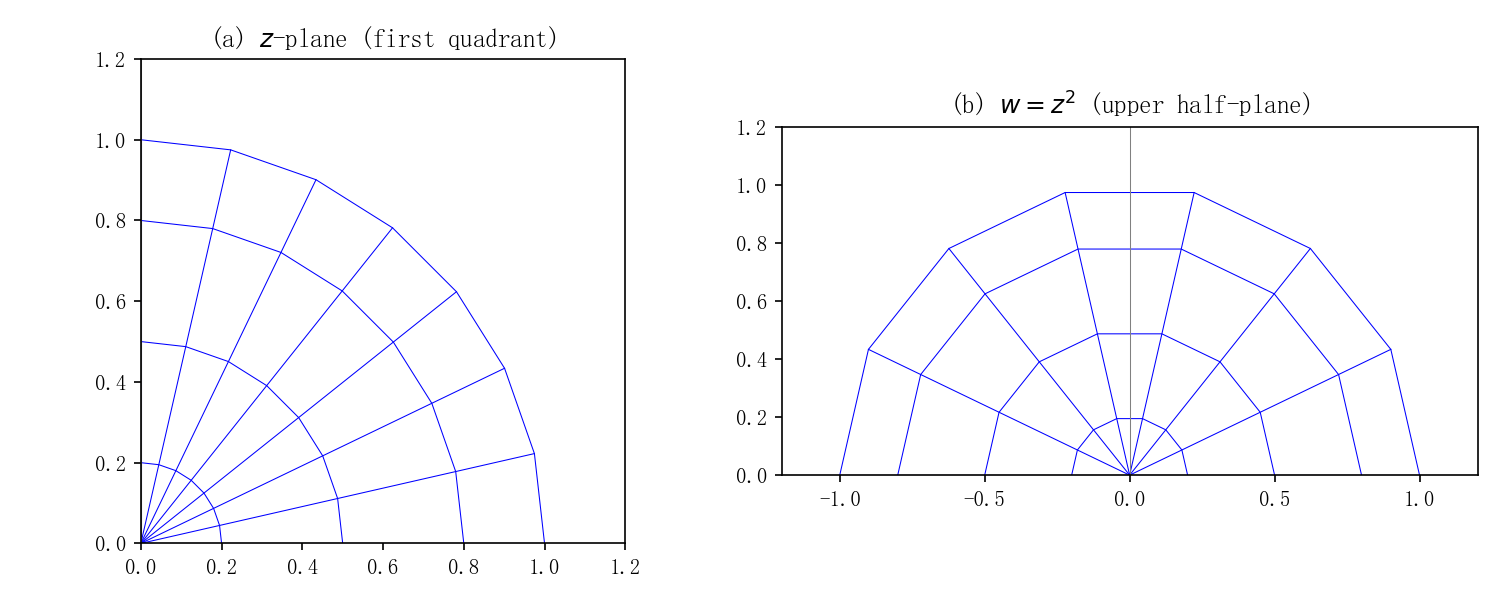
\includegraphics[width=0.75\textwidth]{figures/fig2_3_conformal.png}
\caption{$w=z^2$ 的保角映射：(a) $z$ 平面上的第一象限扇形；(b) 映射后的上半平面 $w$ 平面。注意原先在原点相交于 $90^\circ$ 的边界线变成了 $180^\circ$——因为 $f'(0)=0$，保角性在 $f'(z)=0$ 处失效。}
\label{fig:conformal}
\end{figure}

\subsection{基本映射}

\begin{itemize}
\item $w = z + a$：平移
\item $w = e^{\mathrm{i}\alpha}z$：旋转 $\alpha$
\item $w = kz$：缩放
\item $w = 1/z$：反演（将圆变为圆或直线）
\item $w = z^2$：将角域映射为上半平面
\item $w = \sqrt{z}$：将角域映射为半平面（$z^2$ 的逆映射）
\item $w = e^z$：将水平带形映射为角域
\item $w = \ln z$：将角域映射为带形（$e^z$ 的逆映射）
\end{itemize}

\begin{example}[用保角映射求解静电场]
设有两个半无限平行板电极，电势分别为 $\phi=0$ 和 $\phi=V$，间距 $d$。
映射 $w = e^{\pi z/d}$ 将带形区域 $0<\Im z<d$ 映射为上半平面 $\Im w>0$，而平行板电容器中均匀场的复势 $F(w) = V/\pi\ln w$。最终得到物理平面上的电势分布：
\begin{equation}
\phi(x,y) = \frac{V}{d}\,y,
\qquad
\psi(x,y) = \frac{V}{d}\,x.
\end{equation}
这正是平板电容器的均匀场解。保角映射将复杂边界问题化为标准区域上的已知解。
\end{example}

\subsection{Joukowski 映射与机翼理论}

\textbf{Joukowski 映射：}
\begin{equation}
w = z + \frac{1}{z}.
\label{eq:joukowski}
\end{equation}

这个映射在空气动力学中至关重要——它将圆映射为机翼形状（Joukowski 翼型）。

当 $z = e^{\mathrm{i}\theta}$（单位圆）时，$w = 2\cos\theta$，是实轴上的线段 $[-2,2]$——单位圆被映射为平板。

当 $z = Re^{\mathrm{i}\theta}$（$R>1$，更大的圆）时：
\begin{equation}
w = Re^{\mathrm{i}\theta} + \frac{1}{R}e^{-\mathrm{i}\theta}
= \left(R + \frac{1}{R}\right)\cos\theta + \mathrm{i}\left(R - \frac{1}{R}\right)\sin\theta.
\end{equation}
这是一个椭圆。如果圆心不在原点而在 $(-\varepsilon,0)$，映射得到的曲线就变成了一个具有圆头尖尾的翼型。

\textbf{物理意义：} 绕圆柱的势流解是已知的（复势 $F(z) = U(z + a^2/z)$），通过 Joukowski 映射可以将其变换为绕翼型的流动。这就是\textbf{薄翼理论}的数学基础。

\begin{insight}[保角映射的物理哲学]
保角映射之所以有效，是因为拉普拉斯方程 $\nabla^2\phi=0$ 在解析变换下形式不变。换句话说，\textbf{静电场、稳态热传导、无旋流场、静磁场（无源区）都共享同一数学结构}。当你解出了其中一个问题的保角映射解，就免费得到了所有其他问题的解。这种数学统一性正是物理学家追求的境界。
\end{insight}

\subsection{Schwarz-Christoffel 映射}

\textbf{Schwarz-Christoffel 映射}将上半平面映射到任意多边形内部：
\begin{equation}
w = A\int_{z_0}^{z} (\zeta - x_1)^{\alpha_1-1}(\zeta - x_2)^{\alpha_2-1}\cdots(\zeta - x_n)^{\alpha_n-1}\,\dd\zeta + B,
\label{eq:sc_mapping}
\end{equation}
其中 $\alpha_k\pi$ 是多边形在顶点 $w_k$ 处的内角，$x_k$ 是实轴上对应顶点的原像点。

\begin{example}[直角区域的映射]
考虑映射 $w = \sqrt{z}$。它将上半平面映射为第一象限（一个 $90^\circ$ 角域）。这是 Schwarz-Christoffel 映射在 $n=2$ 时的特例——两个顶点分别在 $0$ 和无穷远，内角均为 $\pi/2$。

在静电学中，这个映射用来求解导体尖角附近的电场分布——尖角处的场强会发散（尖端放电效应），这正是 $\sqrt{z}$ 在 $z=0$ 处导数无穷大的物理表现。
\end{example}

\section{解析函数的物理应用专题}
\label{sec:physics_applications}

\subsection{二维拉普拉斯场的复势}

二维静电场和不可压缩无旋流场可以用复势统一描述。设 $\phi$ 为势函数，$\psi$ 为流函数：
\begin{equation}
F(z) = \phi(x,y) + \mathrm{i}\psi(x,y),\quad
F'(z) = E_x - \mathrm{i}E_y \quad(\text{电场情形}).
\end{equation}

\textbf{物理量对应关系：}
\begin{itemize}
\item $\phi$ = 电势 / 速度势
\item $\psi$ = 流函数（$\nabla\psi$ 旋转 $90^\circ$ 给出场方向）
\item $F'(z)$ = 共轭场强 / 复速度
\end{itemize}

\begin{example}[点源的复势]
位于原点的二维点源（强度 $\lambda$）的复势为：
\begin{equation}
F(z) = \frac{\lambda}{2\pi}\ln z
= \frac{\lambda}{2\pi}(\ln r + \mathrm{i}\theta).
\end{equation}
实部 $\phi = \lambda/(2\pi)\ln r$ 是二维泊松方程的解，对应于无限长线电荷的电势。虚部 $\theta$ 是流函数——流线从原点径向发出。
\end{example}

\begin{example}[电偶极子的复势]
位于 $\pm d/2$ 的一对点源和点汇（强度分别为 $\pm\lambda$）构成偶极子。当 $d\to0$ 时保持 $\lambda d = p$ 有限，复势为：
\begin{equation}
F(z) = \frac{p}{2\pi z}.
\end{equation}
这是二维电偶极子的复势。对应的电场 $E_x - \mathrm{i}E_y = F'(z) = -\frac{p}{2\pi z^2}$。等势线 $\Re(F) = \text{常数}$ 是一族通过原点的圆。
\end{example}

\begin{example}[均匀流绕圆柱]
在均匀流 $U$ 中放置半径为 $a$ 的圆柱，复势为：
\begin{equation}
F(z) = U\left(z + \frac{a^2}{z}\right).
\end{equation}
验证：大 $|z|$ 时 $F(z) \sim Uz$（均匀流），在 $|z|=a$ 处 $\Im(F) = U(r - a^2/r)\sin\theta = 0$，即圆柱表面是一条流线。
\end{example}

\subsection{色散关系与 Kramers-Kronig 关系}

\textbf{因果律 + 解析性 = 色散关系。} 这是复变函数在物理中最深刻的应用之一。

设 $\chi(\omega) = \chi'(\omega) + \mathrm{i}\chi''(\omega)$ 为线性响应函数的频域表示（如介电函数、磁导率、电导率）。因果性要求 $\chi(t)=0$ 对 $t<0$，这导致 $\chi(\omega)$ 在上半复 $\omega$ 平面解析。

对上半平面应用柯西积分公式，取实部和虚部即得 Kramers-Kronig 关系：
\begin{align}
\chi'(\omega) &= \frac{1}{\pi}\mathcal{P}\int_{-\infty}^{\infty}
\frac{\chi''(\omega')}{\omega' - \omega}\,\dd\omega',\\
\chi''(\omega) &= -\frac{1}{\pi}\mathcal{P}\int_{-\infty}^{\infty}
\frac{\chi'(\omega')}{\omega' - \omega}\,\dd\omega'.
\label{eq:kk_relations}
\end{align}

\begin{example}[洛伦兹振子模型]
对于洛伦兹振子模型（经典色散理论），介电函数为：
\begin{equation}
\varepsilon(\omega) = 1 + \frac{\omega_p^2}{\omega_0^2 - \omega^2 - \mathrm{i}\gamma\omega}.
\end{equation}

实部和虚部分别为：
\begin{align}
\varepsilon'(\omega) &= 1 + \frac{\omega_p^2(\omega_0^2 - \omega^2)}{(\omega_0^2 - \omega^2)^2 + \gamma^2\omega^2},\\
\varepsilon''(\omega) &= \frac{\omega_p^2\gamma\omega}{(\omega_0^2 - \omega^2)^2 + \gamma^2\omega^2}.
\end{align}

可以验证这对 $(\varepsilon',\varepsilon'')$ 满足 Kramers-Kronig 关系。在共振频率 $\omega_0$ 附近，$\varepsilon''$ 出现峰值（吸收），而 $\varepsilon'$ 急剧变化（反常色散）。
\end{example}

\begin{insight}
Kramers-Kronig 关系的物理意义振聋发聩：\textbf{如果只知道某个频率下材料的吸收谱（$\chi''$ 的虚部），就可以唯一地计算出色散（$\chi'$ 的实部）}。反之亦然。这意味着"吸收"和"色散"不是独立的物质性质——它们是同一个解析函数在实轴上的实部和虚部。光学中折射率和消光系数的关系、粒子物理中 forward scattering 的色散关系，都源于此。
\end{insight}

\subsection{线性系统的传递函数与解析性}

在线性系统理论中，传递函数 $H(s)$ 是 $s$ 的复变函数。系统的因果性等价于 $H(s)$ 的收敛域（ROC）是某个右半平面。稳定性等价于 $H(s)$ 的所有极点具有负实部（即位于左半平面）。

\begin{example}[RC 低通滤波器的传递函数]
\begin{equation}
H(s) = \frac{1}{1 + sRC},\quad \Re(s) > -\frac{1}{RC}.
\end{equation}
极点在 $s = -1/(RC)$（左半平面），因此系统稳定。单位冲激响应为：
\begin{equation}
h(t) = \frac{1}{RC}e^{-t/(RC)}\Theta(t).
\end{equation}
验证因果性：$t<0$ 时 $h(t)=0$。
\end{example}

\subsection{傅里叶变换与解析延拓}

拉普拉斯变换 $F(s)$ 是傅里叶变换 $\tilde{f}(\omega)$ 的解析延拓：
\begin{equation}
F(\sigma + \mathrm{i}\omega) = \int_0^{\infty} f(t) e^{-\sigma t} e^{-\mathrm{i}\omega t}\,\dd t.
\end{equation}

当 $\sigma=0$ 时退化为傅里叶变换（如果收敛）。这个联系表明：\textbf{拉普拉斯变换 = 傅里叶变换 + 收敛因子}。这正是第 3 章的核心内容之一。

\section{本章小结}

\begin{itemize}
\item \textbf{复数与相量法} 将时域微积分化为频域代数，是线性系统分析的利器。
\item \textbf{柯西-黎曼方程} 是解析函数的定义性特征，它将解析函数与二维拉普拉斯场紧密联系。
\item \textbf{柯西积分定理与公式} 表明解析函数具有"边界决定内部"的刚性。
\item \textbf{留数定理} 将围道积分化为留数求和，是计算实积分和反常积分的标准工具。
\item \textbf{保角映射} 将复杂几何边界的物理问题映射到标准区域求解。
\item \textbf{解析性与因果性} 的结合导出 Kramers-Kronig 关系，是所有线性响应系统的普适约束。
\end{itemize}

\subsection*{概念图谱}

\begin{center}
\fbox{\parbox{0.92\textwidth}{
\textbf{复变函数的概念网络：}\\[3pt]
$\bullet$ 复数代数 $\to$ 相量法（交流电路）\\[3pt]
$\bullet$ 柯西-黎曼方程 $\to$ 调和函数 $\to$ 二维场（静电/流体）$\to$ 复势 \\[3pt]
$\bullet$ 柯西积分定理 $\to$ 柯西积分公式 $\to$ 高阶导数公式 $\to$ 泊松积分公式\\[3pt]
$\bullet$ 洛朗展开 $\to$ 留数 $\to$ 留数定理 $\to$ 实积分计算 / Kramers-Kronig 关系\\[3pt]
$\bullet$ 解析函数 $\to$ 保角映射 $\to$ 二维边值问题统一解法\\[3pt]
$\bullet$ 多值函数 $\to$ 黎曼曲面 $\to$ 割线围道积分
}}
\end{center}

\subsection*{公式参考表}

\begin{table}[h]
\centering
\caption{复变函数核心公式速查}
\label{tab:complex_formulas}
\begin{tabular}{c|c}
\toprule
公式 & 说明 \\
\midrule
$e^{\mathrm{i}\theta} = \cos\theta + \mathrm{i}\sin\theta$ & 欧拉公式 \\
$\frac{\partial u}{\partial x} = \frac{\partial v}{\partial y},\; \frac{\partial u}{\partial y} = -\frac{\partial v}{\partial x}$ & 柯西-黎曼方程 \\
$\oint_C f(z)\,\dd z = 0$（$f$ 在 $C$ 内解析） & 柯西积分定理 \\
$f(z_0) = \frac{1}{2\pi\mathrm{i}}\oint_C \frac{f(z)}{z-z_0}\,\dd z$ & 柯西积分公式 \\
$f^{(n)}(z_0) = \frac{n!}{2\pi\mathrm{i}}\oint_C \frac{f(z)}{(z-z_0)^{n+1}}\,\dd z$ & 高阶导数公式 \\
$\oint_C f(z)\,\dd z = 2\pi\mathrm{i}\sum\mathop{\mathrm{Res}} f(z_k)$ & 留数定理 \\
$\mathop{\mathrm{Res}}_{z=z_0} f = \lim_{z\to z_0}(z-z_0)f(z)$ & 一阶极点留数 \\
$\mathop{\mathrm{Res}}_{z=z_0} f = \frac{1}{(m-1)!}\lim_{z\to z_0}\frac{d^{m-1}}{dz^{m-1}}[(z-z_0)^m f(z)]$ & $m$ 阶极点留数 \\
$w = z + 1/z$ & Joukowski 映射 \\
$\chi'(\omega) = \frac{1}{\pi}\mathcal{P}\int\frac{\chi''(\omega')}{\omega'-\omega}\,\dd\omega'$ & Kramers-Kronig 关系 \\
\bottomrule
\end{tabular}
\end{table}

\begin{insight}
回顾第 2 章，你会发现一条主线：\textbf{从复数的代数引入 $\to$ 解析函数的微分约束 $\to$ 整体积分性质 $\to$ 留数与奇点结构 $\to$ 物理应用}。这与第 1 章中"局部微分 $\to$ 整体积分"的思维模式一脉相承。在复变函数的语境中，局部就是柯西-黎曼方程，整体就是留数定理。
\end{insight}

\section*{习题}

\textbf{基础题（巩固概念）}

\begin{enumerate}
\item 将复数 $z = 1 + \mathrm{i}\sqrt{3}$ 化为极坐标形式 $re^{\mathrm{i}\theta}$。计算 $z^{10}$。
\item 计算下列复数的实部、虚部、模和辐角主值：
(1) $(1+\mathrm{i})^3$；(2) $\frac{1-\mathrm{i}}{1+\mathrm{i}}$；(3) $e^{2+\mathrm{i}\pi/3}$。
\item 判断下列函数在何处可导，在何处解析：
(1) $f(z) = \bar{z}^2$；(2) $f(z) = e^z$；(3) $f(z) = \Re(z)$；
(4) $f(z) = \sin z$。
\item 验证 $u(x,y) = e^x\cos y$ 是调和函数，并求其共轭调和函数 $v(x,y)$，写出 $f(z)=u+\mathrm{i}v$ 的显式表达式。
\item 计算 $\displaystyle\int_C \frac{\dd z}{z-1}$，$C$ 为 $|z-1|=1$ 的逆时针圆周。
\item 求 $f(z) = \frac{z}{(z-1)(z-2)}$ 在 $z=1$ 和 $z=2$ 处的留数。
\end{enumerate}

\textbf{提高题（应用分析）}

\begin{enumerate}
\item[7.] 利用留数定理计算 $\displaystyle\int_0^{2\pi}\frac{\dd\theta}{a+\cos\theta}$（$a>1$）。写出完整步骤并验证结果的合理性（当 $a\to\infty$ 时积分应趋近于 0）。
\item[8.] 计算 $\displaystyle\int_{-\infty}^{\infty}\frac{x^2}{x^4+1}\,\dd x$。\textbf{提示：} 分母有四个一阶极点 $e^{\mathrm{i}\pi/4}, e^{3\mathrm{i}\pi/4}, e^{5\mathrm{i}\pi/4}, e^{7\mathrm{i}\pi/4}$，只取上半平面的两个。
\item[9.] 求映射 $w = z + 1/z$ 将单位圆 $|z|=1$ 映射为什么曲线？该映射在二维理想流体的圆柱绕流问题中有何应用？\textbf{提示：} $z=e^{\mathrm{i}\theta}$ 时 $w = 2\cos\theta$ 是实轴上的线段。
\item[10.] 计算洛朗展开：在 $z=0$ 附近将 $f(z) = \frac{1}{z(z-1)}$ 展开为洛朗级数。分别在 $0<|z|<1$ 和 $|z|>1$ 两个区域写出展开式。
\item[11.] 求 RC 串联电路（$C=10\mu\text{F}$, $R=1\text{k}\Omega$）的传递函数、截止频率和幅频响应 $|H(\omega)|$ 的表达式。当输入 $V_{\text{in}}(t) = 10\cos(100t)$ 时，求稳态输出。
\item[12.] 计算 $\displaystyle\int_0^{\infty} \frac{\sin x}{x}\,\dd x = \frac{\pi}{2}$ 用 Jordan 引理和围道积分验证。
\end{enumerate}

\textbf{挑战题（综合拓展）}

\begin{enumerate}
\item[13.]（双线性变换）映射 $w = \frac{z-1}{z+1}$ 将右半平面 $\Re(z)>0$ 映射到单位圆 $|w|<1$。证明这一性质。该映射在控制理论中用于将 $s$ 平面的稳定性边界映射到 $z$ 平面的单位圆。
\item[14.]（Kramers-Kronig 练习）设 $\chi''(\omega) = \frac{\omega}{1+\omega^2}$，利用 Kramers-Kronig 关系求 $\chi'(\omega)$。\textbf{提示：} 用留数定理计算主值积分。验证你的结果满足 $\chi(-\omega) = \chi^*(\omega)$（实信号的对称性）。
\item[15.]（量子散射）一维薛定谔方程的一个解为 $\psi(x) \sim e^{\mathrm{i}kx} + f(k)\frac{e^{\mathrm{i}k|x|}}{|x|}$。散射振幅 $f(k)$ 在复 $k$ 平面上有极点 $k=\mathrm{i}\kappa$（$\kappa>0$），证明这对应束缚态，其能量为 $E = -\hbar^2\kappa^2/(2m)$。
\item[16.]（保角映射与传热）一半无限大平板 $x>0$，$y=0$ 边界上温度分布为 $T(x,0)=T_0\Theta(a-|x|)$（即 $|x|<a$ 处 $T=T_0$，其余 $T=0$）。通过适当的保角映射和复势方法，求平板上方的稳态温度分布。
\item[17.]（割线围道积分）计算 $\displaystyle\int_0^{\infty} \frac{\ln x}{1+x^2}\,\dd x$。\textbf{提示：} 考虑 $f(z) = \frac{(\ln z)^2}{1+z^2}$ 的围道积分，取割线沿正实轴。
\item[18.]（Joukowski 翼型）设 $z$ 平面上的圆为 $|z - \varepsilon| = 1 + \varepsilon$（$\varepsilon>0$ 小量），圆心在 $(\varepsilon,0)$。通过 Joukowski 映射 $w = z + 1/z$ 得到翼型形状。证明翼型在 $w=2$ 处有尖点（后缘），并画出 $\varepsilon=0.1$ 时的翼型轮廓。
\end{enumerate}

% ============================================================
%  第 3 章  积分变换：傅里叶分析与拉普拉斯变换（扩展版）
% ============================================================

\chapter{积分变换：傅里叶分析与拉普拉斯变换}

\section{本章概览与学习路线}

傅里叶变换和拉普拉斯变换是物理学家最重要的两种积分变换工具。它们将函数从时域（或空间域）映射到频域（或复频域），将微分方程转化为代数方程，将卷积转化为乘法。

\begin{center}
\fbox{\parbox{0.9\textwidth}{\centering
\textbf{核心逻辑链条：}\\
周期信号 $\to$ 傅里叶级数（离散谱）$\to$ 非周期信号 $\to$ 傅里叶变换（连续谱）\\
$\to$ 收敛性问题 $\to$ 拉普拉斯变换（复频域）$\to$ 传递函数与系统分析
}}
\end{center}

\subsection*{不同读者的学习路径}

\begin{itemize}
\item \textbf{物理专业学生：} 重点关注 \S3.3（FT 基本性质）、\S3.4（FT 物理应用——衍射、量子力学、不确定性原理）、\S3.5（Laplace 变换求解 ODE）、\S3.6（RLC 电路与传递函数）。
\item \textbf{信号处理/电子工程学生：} 重点关注 \S3.2（傅里叶级数的工程应用）、\S3.3（FT 性质与卷积定理）、\S3.4（采样定理、滤波器设计）、\S3.6（传递函数与稳定性）。
\item \textbf{数学学生：} 重点关注 FT 和 Laplace 变换的严格推导、收敛条件、逆变换的围道积分表示。
\end{itemize}

\section{傅里叶级数}
\label{sec:fourier_series}

\subsection*{动机：为什么周期运动可以分解为谐波？}

伽利略发现摆的周期与振幅无关（小角度下是简谐运动），傅里叶则做了相反的事：任何周期运动都可以看作多个不同频率简谐运动的叠加。这就是说：\textbf{简谐运动不是特例，而是周期运动的基本"砖块"}。

\subsection{周期函数的谐波分解}

设 $f(t)$ 是周期为 $T$ 的函数，在合适的正则条件下可以展开为傅里叶级数：
\begin{equation}
f(t) = \frac{a_0}{2} + \sum_{n=1}^{\infty}
\left[a_n\cos(n\omega_0 t) + b_n\sin(n\omega_0 t)\right],
\label{eq:fourier_series_tri}
\end{equation}
其中 $\omega_0 = 2\pi/T$ 是基频。傅里叶系数由正交性给出：
\begin{align}
a_n &= \frac{2}{T}\int_{-T/2}^{T/2} f(t)\cos(n\omega_0 t)\,\dd t,\\
b_n &= \frac{2}{T}\int_{-T/2}^{T/2} f(t)\sin(n\omega_0 t)\,\dd t.
\end{align}

\textbf{复数形式}（更适合理论分析）：
\begin{equation}
f(t) = \sum_{n=-\infty}^{\infty} c_n e^{\mathrm{i}n\omega_0 t},
\qquad
c_n = \frac{1}{T}\int_{-T/2}^{T/2} f(t)e^{-\mathrm{i}n\omega_0 t}\,\dd t.
\label{eq:fourier_series_complex}
\end{equation}

两种形式的关系：$c_0 = a_0/2$, $c_n = (a_n - \mathrm{i}b_n)/2$, $c_{-n} = (a_n + \mathrm{i}b_n)/2$（$n\geq1$）。

\subsection{收敛条件（Dirichlet 条件）}

傅里叶级数在以下条件下逐点收敛到 $f(t)$：
\begin{itemize}
\item $f(t)$ 在一个周期内绝对可积：$\int_{-T/2}^{T/2} |f(t)|\,\dd t < \infty$。
\item $f(t)$ 在一个周期内只有有限个极值点和有限个间断点。
\end{itemize}
在间断点处，傅里叶级数收敛到左右极限的平均值：$\frac{f(t_0^+) + f(t_0^-)}{2}$。

\begin{example}[方波的傅里叶级数]
周期为 $2\pi$ 的方波：
\begin{equation}
f(t) = \begin{cases}
1, & 0 < t < \pi,\\
-1, & -\pi < t < 0.
\end{cases}
\end{equation}

由于 $f(t)$ 是奇函数，$a_n=0$。计算 $b_n$：
\begin{align*}
b_n &= \frac{1}{\pi}\int_{-\pi}^{\pi} f(t)\sin(nt)\,\dd t
= \frac{2}{\pi}\int_{0}^{\pi} \sin(nt)\,\dd t \\
&= \frac{2}{\pi}\left[-\frac{\cos(nt)}{n}\right]_0^{\pi}
= \frac{2}{n\pi}(1 - \cos n\pi) \\
&= \begin{cases}
4/(n\pi), & n\text{ 奇数},\\
0, & n\text{ 偶数}.
\end{cases}
\end{align*}

因此方波的傅里叶级数为：
\begin{equation}
f(t) = \frac{4}{\pi}\sum_{k=0}^{\infty}\frac{\sin[(2k+1)t]}{2k+1}
= \frac{4}{\pi}\left(\sin t + \frac{1}{3}\sin 3t + \frac{1}{5}\sin 5t + \cdots\right).
\end{equation}
在跳跃点 $t=0,\pm\pi$ 处，级数收敛到 $0$——这正是左右极限的平均值 $(1+(-1))/2=0$。
\end{example}

\begin{example}[锯齿波的傅里叶级数]
周期为 $2\pi$ 的锯齿波：$f(t) = t$, $t\in(-\pi,\pi)$。

由于 $f(t)$ 是奇函数，$a_n=0$。
\begin{align*}
b_n &= \frac{1}{\pi}\int_{-\pi}^{\pi} t\sin(nt)\,\dd t
= \frac{2}{\pi}\int_{0}^{\pi} t\sin(nt)\,\dd t\quad(\text{奇函数}\times\text{奇函数}=\text{偶函数}) \\
&= \frac{2}{\pi}\left[\frac{\sin(nt) - nt\cos(nt)}{n^2}\right]_0^{\pi}
= \frac{2}{\pi}\cdot\frac{-\pi\cos(n\pi)}{n} = \frac{(-1)^{n+1}2}{n}.
\end{align*}

因此：
\begin{equation}
t = 2\sum_{n=1}^{\infty} \frac{(-1)^{n+1}}{n}\sin(nt),\qquad -\pi < t < \pi.
\end{equation}

在 $t=\pm\pi$ 处，级数收敛到 $0$，恰好是 $f(-\pi)$ 和 $f(\pi)$ 的平均值。
\end{example}

\begin{insight}[傅里叶级数的物理意义]
三角函数的正交性 $\int_0^T \cos(n\omega_0 t)\cos(m\omega_0 t)\,\dd t \propto \delta_{nm}$ 保证了这个分解的"唯一性"——每个频率成分是独立的自由度。在振动分析中，$|c_n|^2$ 正比于第 $n$ 阶谐波的能量。这解释了为什么拨动吉他的弦虽然产生的是基频的周期运动，但音色（谐波成分的比例）使不同乐器能够区分。
\end{insight}

% 傅里叶级数逼近图
\begin{figure}[H]
\centering
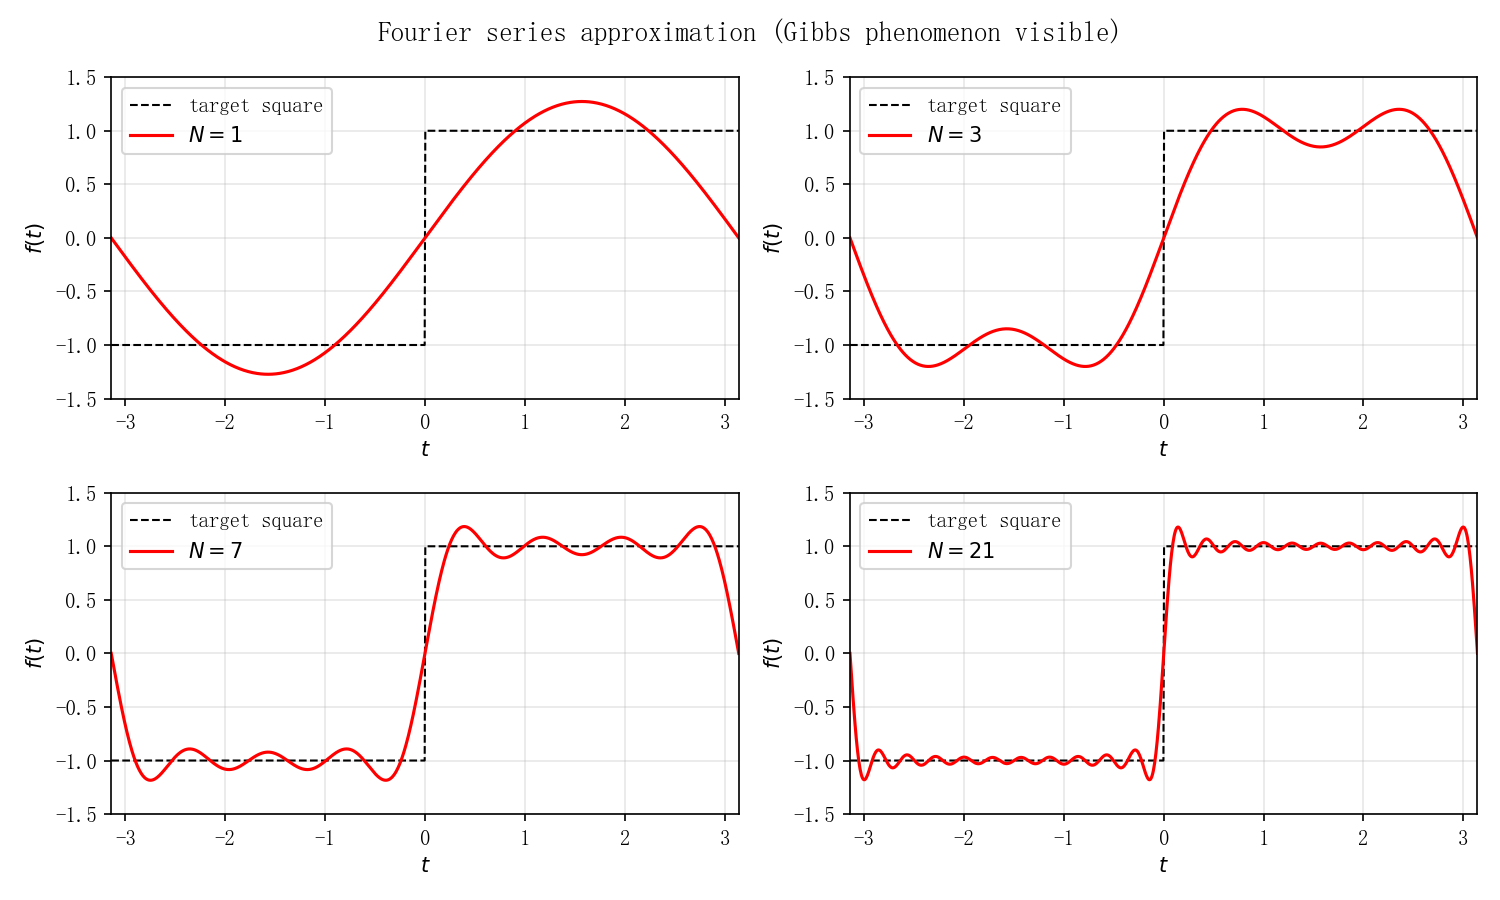
\includegraphics[width=0.8\textwidth]{figures/fig3_1_fourier_series.png}
\caption{傅里叶级数对方波的逼近。$N=1$ 仅含基频，$N=7$ 已较好地近似了方波形状。注意在跳跃点附近出现过冲（吉布斯现象），不随 $N$ 增加而消失。}
\label{fig:fourier_series}
\end{figure}

\subsection{吉布斯现象}

在函数的不连续点附近，傅里叶级数的部分和会出现过冲，这就是\textbf{吉布斯现象 (Gibbs phenomenon)}。过冲幅度约为跳跃高度的 $9\%$，且不随项数增加而消失——它只是越来越逼近跳跃点。

吉布斯现象在信号处理中至关重要：它告诉我们在用有限带宽近似陡峭边沿时，总会存在过冲和振铃。这也暗示了为什么需要在数字信号处理中使用窗函数（如 Hanning、Hamming 窗）来减轻这种效应。

\subsection{傅里叶级数的能量解释}

\textbf{帕塞瓦尔定理（傅里叶级数形式）：}
\begin{equation}
\frac{1}{T}\int_{-T/2}^{T/2} |f(t)|^2\,\dd t
= \frac{a_0^2}{4} + \frac{1}{2}\sum_{n=1}^{\infty}(a_n^2 + b_n^2)
= \sum_{n=-\infty}^{\infty} |c_n|^2.
\label{eq:parseval_series}
\end{equation}

物理意义：信号在一个周期内的平均功率等于各频率成分功率之和。这保证了时域和频域的能量守恒。

\section{傅里叶变换}
\label{sec:fourier_transform}

\subsection*{动机：非周期信号怎么办？}

周期信号用傅里叶级数分解为离散谱，但一个单一的脉冲（如 $\delta$ 函数）没有周期。让周期 $T\to\infty$，离散谱 $n\omega_0$ 变成连续谱 $\omega$——这就是傅里叶变换。

\subsection{从级数到变换}

将周期 $T\to\infty$，频谱从离散变为连续，傅里叶级数过渡为傅里叶变换：
\begin{align}
\tilde{f}(\omega) &= \int_{-\infty}^{\infty} f(t)\,e^{-\mathrm{i}\omega t}\,\dd t,\\
f(t) &= \frac{1}{2\pi}\int_{-\infty}^{\infty} \tilde{f}(\omega)\,e^{\mathrm{i}\omega t}\,\dd\omega.
\label{eq:fourier_transform}
\end{align}

注意对称性：正变换和逆变换只差一个 $1/(2\pi)$ 因子和 $\omega$ 的符号。这种对称性本身就是"时频对偶"的数学表达。

\textbf{另一种常用定义（角频率 $\omega$ vs 频率 $f$）：}
\begin{equation}
\tilde{F}(f) = \int_{-\infty}^{\infty} f(t) e^{-2\pi\mathrm{i}ft}\,\dd t,
\quad
f(t) = \int_{-\infty}^{\infty} \tilde{F}(f) e^{2\pi\mathrm{i}ft}\,\dd f.
\end{equation}
这种定义完全对称——正逆变换的系数都是 $1$。在本书中我们统一使用 $\omega$ 定义。

\subsection{基本性质与推导}

\begin{table}[h]
\centering
\caption{傅里叶变换的基本性质（$\mathcal{F}[f] = \tilde{f}$）}
\label{tab:ft_properties}
\begin{tabular}{c|c}
\toprule
性质 & 变换对 \\
\midrule
线性 & $\mathcal{F}[\alpha f+\beta g] = \alpha\tilde{f}+\beta\tilde{g}$ \\
时移 & $\mathcal{F}[f(t-t_0)] = e^{-\mathrm{i}\omega t_0}\tilde{f}(\omega)$ \\
频移 & $\mathcal{F}[e^{\mathrm{i}\omega_0 t}f(t)] = \tilde{f}(\omega-\omega_0)$ \\
时域微分 & $\mathcal{F}[f'(t)] = \mathrm{i}\omega\tilde{f}(\omega)$ \\
频域微分 & $\mathcal{F}[t f(t)] = \mathrm{i}\tilde{f}'(\omega)$ \\
尺度变换 & $\mathcal{F}[f(at)] = \frac{1}{|a|}\tilde{f}(\omega/a)$ \\
卷积 & $\mathcal{F}[(f*g)(t)] = \tilde{f}(\omega)\,\tilde{g}(\omega)$ \\
帕塞瓦尔 & $\int |f|^2\,\dd t = \frac{1}{2\pi}\int |\tilde{f}|^2\,\dd\omega$ \\
\bottomrule
\end{tabular}
\end{table}

\textbf{时域微分性质} 尤为重要：它将微分方程化为代数方程。这正是傅里叶变换求解微分方程的关键。卷积定理则是线性系统分析的核心——时域中的卷积对应于频域中的乘法，这意味着系统的输出谱 = 输入谱 × 传递函数。

\begin{example}[傅里叶变换性质的推导：时移性质]
证明 $\mathcal{F}[f(t-t_0)] = e^{-\mathrm{i}\omega t_0}\tilde{f}(\omega)$。

令 $\tau = t - t_0$，则 $t = \tau + t_0$，$\dd t = \dd\tau$：
\begin{align*}
\mathcal{F}[f(t-t_0)]
&= \int_{-\infty}^{\infty} f(t-t_0) e^{-\mathrm{i}\omega t}\,\dd t \\
&= \int_{-\infty}^{\infty} f(\tau) e^{-\mathrm{i}\omega(\tau+t_0)}\,\dd\tau \\
&= e^{-\mathrm{i}\omega t_0}\int_{-\infty}^{\infty} f(\tau) e^{-\mathrm{i}\omega\tau}\,\dd\tau \\
&= e^{-\mathrm{i}\omega t_0}\tilde{f}(\omega).
\end{align*}
物理意义：时域中延迟 $t_0$，频域中增加相位因子 $e^{-\mathrm{i}\omega t_0}$——幅度谱不变，相位谱线性变化。
\end{example}

\begin{example}[傅里叶变换性质的推导：卷积定理]
证明 $\mathcal{F}[(f*g)(t)] = \tilde{f}(\omega)\tilde{g}(\omega)$，其中 $(f*g)(t) = \int_{-\infty}^{\infty} f(\tau)g(t-\tau)\,\dd\tau$。

\begin{align*}
\mathcal{F}[(f*g)(t)]
&= \int_{-\infty}^{\infty} \left[\int_{-\infty}^{\infty} f(\tau)g(t-\tau)\,\dd\tau\right] e^{-\mathrm{i}\omega t}\,\dd t \\
&= \int_{-\infty}^{\infty} f(\tau)\left[\int_{-\infty}^{\infty} g(t-\tau) e^{-\mathrm{i}\omega t}\,\dd t\right]\dd\tau \\
&= \int_{-\infty}^{\infty} f(\tau)\left[e^{-\mathrm{i}\omega\tau}\tilde{g}(\omega)\right]\dd\tau \quad(\text{时移性质}) \\
&= \tilde{g}(\omega)\int_{-\infty}^{\infty} f(\tau) e^{-\mathrm{i}\omega\tau}\,\dd\tau
= \tilde{g}(\omega)\tilde{f}(\omega).
\end{align*}
交换积分次序是证明的关键步骤。
\end{example}

\begin{insight}[时频对偶的物理美感]
傅里叶变换展现出一种深刻的对称性：
\begin{itemize}
\item 时域中的"陡峭"对应频域中的"宽泛"：$\delta$ 函数的变换是常数。
\item 时域中的"宽泛"对应频域中的"陡峭"：常数的变换是 $\delta$ 函数。
\item 时宽-带宽积受不确定关系约束：$\Delta t\,\Delta\omega \geq 1/2$。
\end{itemize}
这正是量子力学中 $\Delta x\,\Delta p \geq \hbar/2$ 的数学根源——位置和动量通过傅里叶变换相联系。
\end{insight}

\subsection{常见函数的傅里叶变换}

\begin{align}
\mathcal{F}[\delta(t)] &= 1,\\
\mathcal{F}[1] &= 2\pi\delta(\omega),\\
\mathcal{F}[e^{-\alpha t}\Theta(t)] &= \frac{1}{\alpha + \mathrm{i}\omega},\quad \Re(\alpha)>0,\\
\mathcal{F}[e^{-at^2}] &= \sqrt{\frac{\pi}{a}}\,e^{-\omega^2/(4a)},\\
\mathcal{F}[\cos(\omega_0 t)] &= \pi[\delta(\omega-\omega_0) + \delta(\omega+\omega_0)],\\
\mathcal{F}[\sin(\omega_0 t)] &= \mathrm{i}\pi[\delta(\omega+\omega_0) - \delta(\omega-\omega_0)].
\end{align}

\textbf{高斯函数的傅里叶变换仍是高斯函数}——这一性质在量子力学中解释为什么高斯波包是最小不确定波包。也意味着高斯函数是傅里叶变换的本征函数。

\begin{example}[矩形脉冲的傅里叶变换]
矩形脉冲 $p_T(t) = \begin{cases} 1, & |t| < T/2, \\ 0, & |t| > T/2. \end{cases}$

\begin{align*}
\tilde{p}_T(\omega) &= \int_{-T/2}^{T/2} 1\cdot e^{-\mathrm{i}\omega t}\,\dd t
= \left[\frac{e^{-\mathrm{i}\omega t}}{-\mathrm{i}\omega}\right]_{-T/2}^{T/2} \\
&= \frac{e^{-\mathrm{i}\omega T/2} - e^{\mathrm{i}\omega T/2}}{-\mathrm{i}\omega}
= \frac{2\sin(\omega T/2)}{\omega} = T\,\mathrm{sinc}\!\left(\frac{\omega T}{2}\right).
\end{align*}

其中 $\mathrm{sinc}\,x = \sin x/x$。注意：脉冲越窄（$T$ 小），频谱越宽——这正是时频对偶性的体现。第一个零点在 $\omega = 2\pi/T$，所以带宽 $\Delta\omega \sim 2\pi/T$，$\Delta t\Delta\omega \sim 2\pi$。
\end{example}

% FT 变换对图
\begin{figure}[H]
\centering
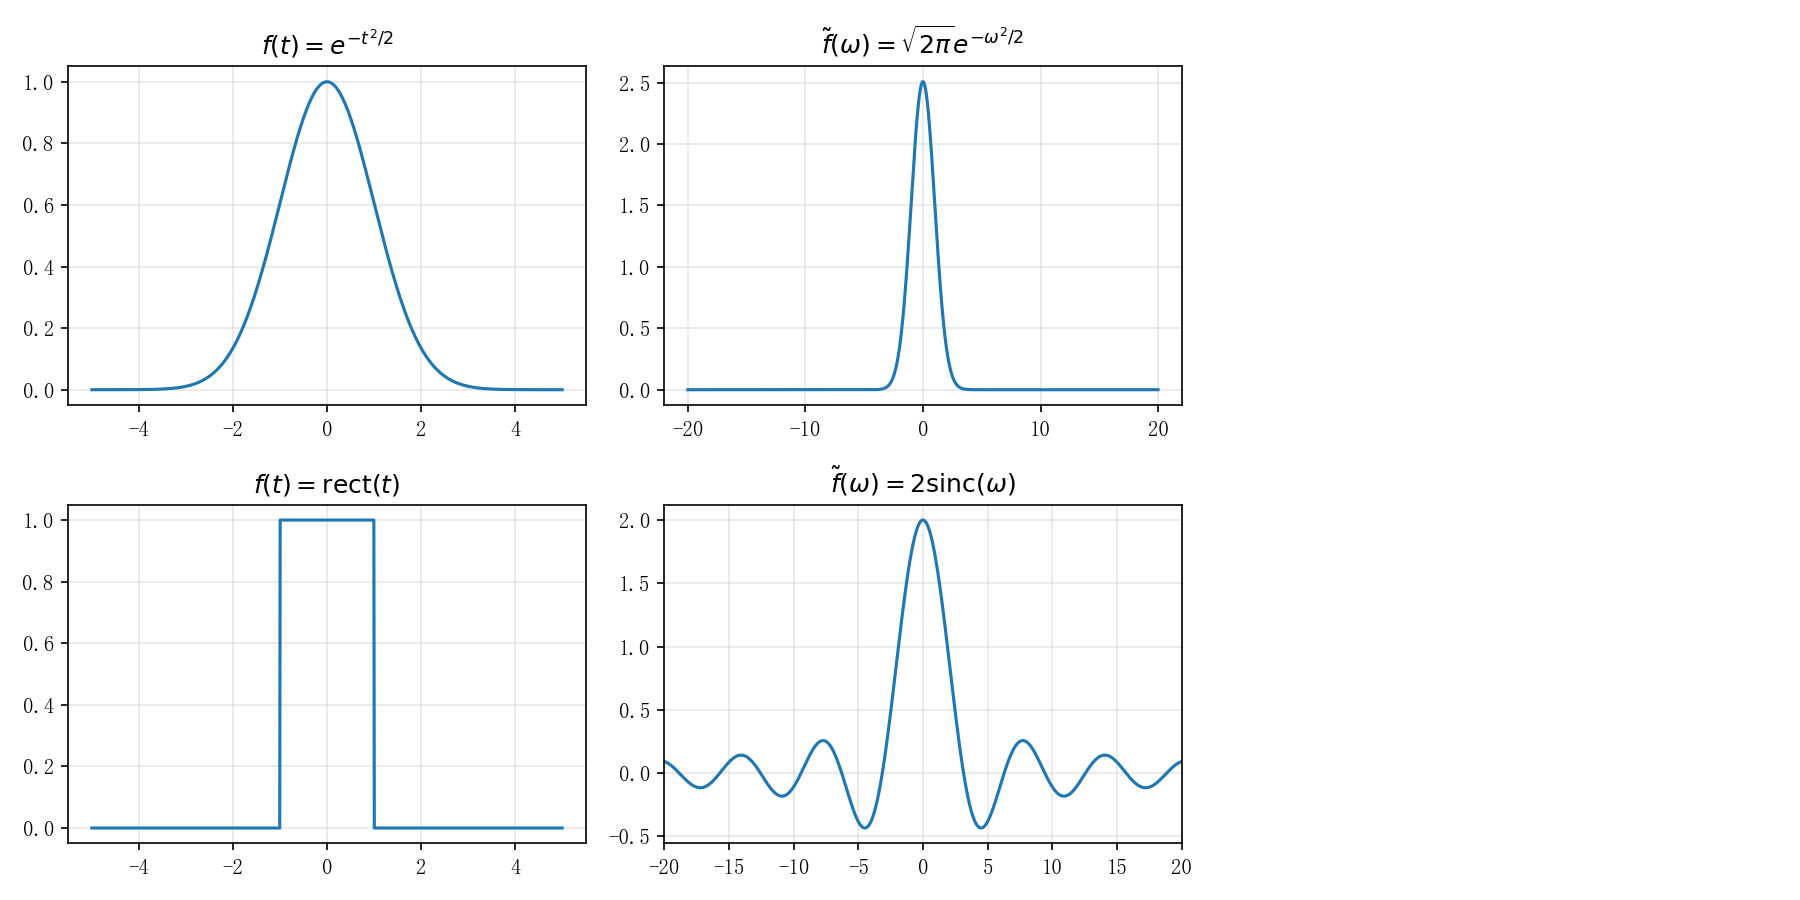
\includegraphics[width=0.85\textwidth]{figures/fig3_2_ft_pairs.png}
\caption{傅里叶变换对示例。上：高斯函数的傅里叶变换仍是高斯。下：矩形脉冲的傅里叶变换是 sinc 函数。注意"窄的时域信号 $\to$ 宽的频域信号"这一对偶性。}
\label{fig:ft_pairs}
\end{figure}

\section{傅里叶变换的物理应用}
\label{sec:ft_physics}

\subsection{衍射与傅里叶光学}

夫琅禾费衍射的光强分布正是孔径函数的傅里叶变换的模平方。单缝衍射：
\begin{equation}
I(\theta) = I_0\,\mathrm{sinc}^2\!\left(\frac{\pi a\sin\theta}{\lambda}\right),
\qquad \mathrm{sinc}\,x = \frac{\sin x}{x}.
\end{equation}

这并非巧合：\textbf{远程衍射图案 = 孔径函数的二维傅里叶变换}。透镜本身就是一个光学傅里叶变换器——物平面和像平面互为傅里叶共轭面。这就是\textbf{傅里叶光学}的核心思想。

\begin{example}[双缝衍射]
双缝间距 $d$，缝宽 $a$。孔径函数是两个矩形函数的卷积：$p_a(x) * [\delta(x-d/2) + \delta(x+d/2)]$。

衍射图案是缝宽衍射和缝间干涉的乘积：
\begin{equation}
I(\theta) = I_0\,\mathrm{sinc}^2\!\left(\frac{\pi a\sin\theta}{\lambda}\right)
\cdot \cos^2\!\left(\frac{\pi d\sin\theta}{\lambda}\right).
\end{equation}

从傅里叶变换角度看：$\mathcal{F}[p_a(x)] \propto \mathrm{sinc}$（单个缝的衍射），$\mathcal{F}[\delta(x-d/2)+\delta(x+d/2)] \propto \cos$（双缝干涉）。卷积的 FT = FT 的乘积，所以衍射图案是两者的乘积！
\end{example}

\begin{insight}
物理光学中最令人惊叹的对应关系：
\begin{itemize}
\item 窄狭缝 $\to$ 宽的衍射图案（窄时域 $\to$ 宽频域）
\item 双缝 $\to$ 双光束干涉（两个 $\delta$ 函数的傅里叶变换是余弦条纹）
\item 光栅 $\to$ 分立谱线（周期结构的变换是离散谱）
\end{itemize}
每一种衍射现象都可以从傅里叶变换的角度获得更深刻的理解。
\end{insight}

\subsection{采样定理与信号处理}

\textbf{采样定理 (Nyquist-Shannon)}：若 $f(t)$ 的最高频率成分为 $f_{\max}$，则采样频率必须 $\geq 2f_{\max}$ 才能无失真地重建原信号。这是模拟-数字转换的基础。

\textbf{证明思路：} 设 $f(t)$ 的频谱在 $|\omega| > \Omega$ 时为零（即带限信号）。以间隔 $T = \pi/\Omega$ 采样得到 $f_s(t) = f(t)\sum_{n=-\infty}^{\infty}\delta(t-nT)$。

采样信号的频谱是原频谱的周期延拓：
\begin{equation}
\tilde{f}_s(\omega) = \frac{1}{T}\sum_{n=-\infty}^{\infty} \tilde{f}(\omega - n\omega_s),\quad \omega_s = \frac{2\pi}{T}.
\end{equation}

只要 $\omega_s \geq 2\Omega$（即 $T \leq \pi/\Omega$），频谱不会混叠，可以通过低通滤波器完美恢复原信号。

\textbf{重建公式：}
\begin{equation}
f(t) = \sum_{n=-\infty}^{\infty} f(nT)\,\mathrm{sinc}\!\left(\frac{\pi t}{T} - n\pi\right).
\end{equation}

\textbf{滤波器设计：} 在频域中设计滤波器是直观的——保留需要的频率成分，抑制不需要的。理想低通滤波器的时域响应是 $\mathrm{sinc}$ 函数，这正是傅里叶变换对 $(\text{矩形窗} \leftrightarrow \text{sinc})$ 的体现。

% FFT 示例图
\begin{figure}[H]
\centering
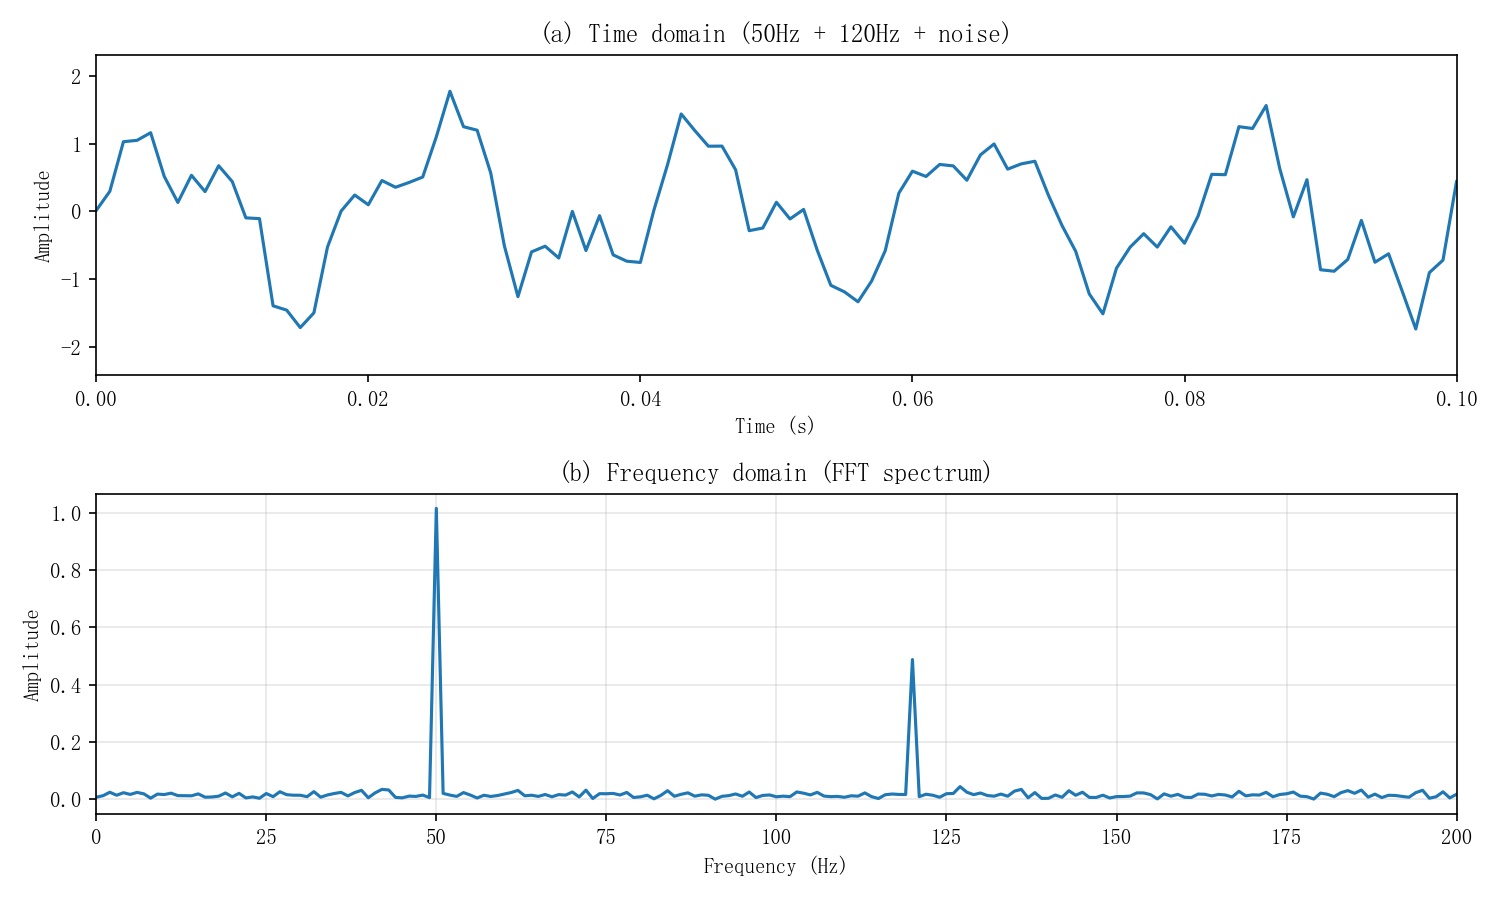
\includegraphics[width=0.8\textwidth]{figures/fig3_3_fft_example.png}
\caption{FFT 频谱分析示例。上：包含 50 Hz 正弦、120 Hz 正弦和噪声的时域信号。下：FFT 振幅谱，50 Hz 和 120 Hz 处清晰可见的峰值。}
\label{fig:fft_example}
\end{figure}

\subsection{量子力学中的动量空间}

波函数在坐标表象和动量表象之间通过傅里叶变换相联系：
\begin{equation}
\tilde{\psi}(p) = \frac{1}{\sqrt{2\pi\hbar}}\int_{-\infty}^{\infty}
\psi(x)\,e^{-\mathrm{i}px/\hbar}\,\dd x.
\end{equation}

动量算符 $\hat{p} = -\mathrm{i}\hbar\partial_x$ 在动量表象中变为乘法算符 $\hat{p} = p$。傅里叶变换在此完成了\textbf{表象变换}的功能——这正是量子力学的数学框架的核心。

\subsection{不确定性原理}

傅里叶变换的时宽-带宽积约束直接导致量子力学中的不确定性原理。

定义时宽 $\Delta t$ 和频宽 $\Delta\omega$：
\begin{align}
(\Delta t)^2 &= \frac{\int (t - \langle t\rangle)^2 |f(t)|^2\,\dd t}{\int |f(t)|^2\,\dd t},\\
(\Delta\omega)^2 &= \frac{\int (\omega - \langle\omega\rangle)^2 |\tilde{f}(\omega)|^2\,\dd\omega}{\int |\tilde{f}(\omega)|^2\,\dd\omega}.
\end{align}

可以证明 $\Delta t \cdot \Delta\omega \geq 1/2$。将 $\omega = p/\hbar$ 代入，得 $\Delta x \cdot \Delta p \geq \hbar/2$。

\textbf{证明（概要）：} 利用施瓦兹不等式：
\begin{align}
\left(\int |f|^2\,\dd t\right)^2
&\leq \int |t f(t)|^2\,\dd t \cdot \int |f'(t)|^2\,\dd t \\
&\leq \Delta t^2 \cdot (\Delta\omega)^2 \cdot \left(\int |f|^2\,\dd t\right)^2.
\end{align}

等号当且仅当 $f(t) \propto e^{-at^2}$（高斯函数）时成立——这正是最小不确定波包。

\subsection{帕塞瓦尔定理与能量守恒}

帕塞瓦尔定理的物理形式：
\begin{equation}
\int_{-\infty}^{\infty} |f(t)|^2\,\dd t
= \frac{1}{2\pi}\int_{-\infty}^{\infty} |\tilde{f}(\omega)|^2\,\dd\omega.
\label{eq:parseval}
\end{equation}

在电学中，左端是信号在时域的总能量，右端是各频率成分的能量之和。能量守恒要求在时域和频域中一致——帕塞瓦尔定理正是这一要求的数学保证。

\subsection{希尔伯特变换与解析信号}

对于实信号 $f(t)$，定义其\textbf{希尔伯特变换}：
\begin{equation}
\hat{f}(t) = \frac{1}{\pi}\mathcal{P}\int_{-\infty}^{\infty} \frac{f(\tau)}{t-\tau}\,\dd\tau.
\end{equation}

在频域中，希尔伯特变换等价于相位移动 $\pm\pi/2$：$\mathcal{F}[\hat{f}](\omega) = -\mathrm{i}\,\mathrm{sgn}(\omega)\tilde{f}(\omega)$。

\textbf{解析信号：} $f_a(t) = f(t) + \mathrm{i}\hat{f}(t)$ 是频域中仅含正频率成分的信号。解析信号在通信理论中用于：
\begin{itemize}
\item 提取瞬时幅度和瞬时相位：$A(t) = |f_a(t)|$, $\phi(t) = \arg f_a(t)$。
\item 定义瞬时频率：$\omega(t) = \phi'(t)$。
\item 单边带调制（SSB）。
\end{itemize}

\section{拉普拉斯变换}
\label{sec:laplace}

\subsection*{动机：傅里叶变换做不到的事情}

傅里叶变换要求函数绝对可积——这对 $e^{t}$、常数函数、甚至 $t^n$ 都不成立。更关键的是，傅里叶变换不自然处理初始条件。拉普拉斯变换通过引入衰减因子 $e^{-\sigma t}$ 解决了这两个问题。

\subsection{从傅里叶到拉普拉斯}

傅里叶变换要求函数在 $\pm\infty$ 绝对可积，许多重要函数（如 $e^{\alpha t}\Theta(t)$ 当 $\alpha>0$、常数函数、多项式）不满足这一条件。引入衰减因子 $e^{-\sigma t}$（$\sigma>0$）迫使积分收敛：
\begin{equation}
\mathcal{L}[f(t)] = F(s)
= \int_0^{\infty} f(t)\,e^{-st}\,\dd t,\qquad s = \sigma + \mathrm{i}\omega.
\label{eq:laplace_transform}
\end{equation}

这是\textbf{单边拉普拉斯变换}，积分下限 $0^-$ 包含原点处的奇异性。相比傅里叶变换，拉普拉斯变换有两个优势：
\begin{itemize}
\item 收敛范围更广（通过 $\sigma$ 控制）。
\item 自然处理初始条件——这是求解初值问题的关键。
\end{itemize}

\subsection{收敛域 (ROC)}

拉普拉斯变换的收敛域是复 $s$ 平面上使得积分收敛的 $\sigma$ 的范围。对于因果信号 $f(t)\Theta(t)$，ROC 是某个 $\sigma > \sigma_c$ 的半平面。

\begin{example}[完整算例：$e^{at}\Theta(t)$ 的拉普拉斯变换]
计算 $\mathcal{L}[e^{at}\Theta(t)]$，$a$ 为实数。

\textbf{步骤 1：写出定义式。}
\begin{equation}
F(s) = \int_0^{\infty} e^{at} e^{-st}\,\dd t
= \int_0^{\infty} e^{-(s-a)t}\,\dd t.
\end{equation}

\textbf{步骤 2：判断收敛性。}
令 $s = \sigma + \mathrm{i}\omega$，$e^{-(s-a)t} = e^{-(\sigma-a)t}e^{-\mathrm{i}\omega t}$。
积分收敛当且仅当 $\sigma - a > 0$，即 $\Re(s) > a$。

\textbf{步骤 3：计算积分。}
当 $\Re(s) > a$ 时：
\begin{equation}
F(s) = \int_0^{\infty} e^{-(s-a)t}\,\dd t
= \left[-\frac{e^{-(s-a)t}}{s-a}\right]_0^{\infty}
= \frac{1}{s-a}.
\end{equation}

\textbf{结论：}
\begin{equation}
\boxed{\;\mathcal{L}[e^{at}\Theta(t)] = \frac{1}{s-a},\quad \Re(s) > a\;}.
\end{equation}
特例：$a=0$ 时 $\mathcal{L}[\Theta(t)] = 1/s$，$\Re(s) > 0$。
\end{example}

\begin{example}[{$\mathcal{L}[\sin(\omega_0 t)\Theta(t)]$} 的推导]
利用欧拉公式 $\sin(\omega_0 t) = (e^{\mathrm{i}\omega_0 t} - e^{-\mathrm{i}\omega_0 t})/(2\mathrm{i})$：
\begin{align*}
\mathcal{L}[\sin(\omega_0 t)\Theta(t)]
&= \frac{1}{2\mathrm{i}}\left[\frac{1}{s-\mathrm{i}\omega_0} - \frac{1}{s+\mathrm{i}\omega_0}\right] \\
&= \frac{1}{2\mathrm{i}}\frac{s+\mathrm{i}\omega_0 - s + \mathrm{i}\omega_0}{s^2 + \omega_0^2}
= \frac{\omega_0}{s^2 + \omega_0^2}.
\end{align*}
ROC: $\Re(s) > 0$。类似可得 $\mathcal{L}[\cos(\omega_0 t)\Theta(t)] = s/(s^2+\omega_0^2)$。
\end{example}

\subsection{拉普拉斯变换的基本性质}

\begin{table}[h]
\centering
\caption{拉普拉斯变换的基本性质}
\label{tab:lt_properties}
\begin{tabular}{c|c}
\toprule
性质 & 变换对 \\
\midrule
时域微分 & $\mathcal{L}[f'(t)] = sF(s) - f(0^-)$ \\
二阶微分 & $\mathcal{L}[f''(t)] = s^2F(s) - sf(0^-) - f'(0^-)$ \\
时域积分 & $\mathcal{L}[\int_0^t f(\tau)\,\dd\tau] = F(s)/s$ \\
频移 & $\mathcal{L}[e^{at}f(t)] = F(s-a)$ \\
时移 & $\mathcal{L}[f(t-a)\Theta(t-a)] = e^{-as}F(s)$ \\
卷积 & $\mathcal{L}[(f*g)(t)] = F(s)G(s)$ \\
初值定理 & $\lim_{t\to0^+} f(t) = \lim_{s\to\infty} sF(s)$ \\
终值定理 & $\lim_{t\to\infty} f(t) = \lim_{s\to0} sF(s)$（极点均在左半平面） \\
\bottomrule
\end{tabular}
\end{table}

\textbf{时域微分性质}是拉普拉斯变换求解 ODE 的关键——它将微分方程转化为代数方程，同时自动引入初始条件。

\begin{proof}[二阶微分性质的推导]
先应用一次微分性质：
\begin{align*}
\mathcal{L}[f''(t)] &= s\mathcal{L}[f'(t)] - f'(0^-) \\
&= s[sF(s) - f(0^-)] - f'(0^-) \\
&= s^2F(s) - sf(0^-) - f'(0^-).
\end{align*}
依此类推，$n$ 阶导数的拉普拉斯变换为：
\begin{equation}
\mathcal{L}[f^{(n)}(t)] = s^nF(s) - s^{n-1}f(0^-) - \cdots - f^{(n-1)}(0^-).
\end{equation}
\end{proof}

\subsection{逆变换与部分分式展开法}

拉普拉斯逆变换的公式为：
\begin{equation}
f(t) = \frac{1}{2\pi\mathrm{i}}\int_{\sigma_0-\mathrm{i}\infty}^{\sigma_0+\mathrm{i}\infty}
F(s)\,e^{st}\,\dd s,
\label{eq:inverse_laplace}
\end{equation}
其中 $\sigma_0$ 位于 ROC 内。该积分可以用留数定理计算。

\textbf{部分分式展开法} 是工程中更常用的方法：将 $F(s)$ 分解为低阶项之和，查表得逆变换。

\begin{example}[部分分式展开的通用方法]
设 $F(s) = \frac{N(s)}{D(s)}$，分母次数高于分子次数。

\textbf{情况 1：所有根为单根。}
$D(s) = (s-p_1)(s-p_2)\cdots(s-p_n)$。
\begin{equation}
\frac{N(s)}{D(s)} = \sum_{k=1}^n \frac{A_k}{s-p_k},\quad
A_k = \lim_{s\to p_k} (s-p_k)\frac{N(s)}{D(s)}.
\end{equation}

\textbf{情况 2：有重根。}
若 $p_1$ 是 $m$ 重根：
\begin{equation}
\frac{N(s)}{(s-p_1)^m\cdots} = \frac{A_{1,m}}{(s-p_1)^m} + \frac{A_{1,m-1}}{(s-p_1)^{m-1}} + \cdots + \frac{A_{1,1}}{s-p_1} + \cdots,
\end{equation}
其中 $A_{1,k} = \frac{1}{(k-1)!}\lim_{s\to p_1}\frac{\dd^{k-1}}{\dd s^{k-1}}\left[(s-p_1)^m\frac{N(s)}{D(s)}\right]$。

\textbf{情况 3：共轭复根。}
保留为二次项形式 $\frac{As+B}{(s+\alpha)^2+\beta^2}$，对应时域中的衰减正弦/余弦。
\end{example}

\begin{example}[完整算例：用拉普拉斯变换解一阶微分方程]
求解 $y' + 2y = e^{-t}$，$y(0)=1$。

\textbf{步骤 1：两边做拉普拉斯变换。}
$\mathcal{L}[y'] + 2\mathcal{L}[y] = \mathcal{L}[e^{-t}]$。
$sY(s) - y(0) + 2Y(s) = \frac{1}{s+1}$。

\textbf{步骤 2：代入初始条件。}
$sY(s) - 1 + 2Y(s) = \frac{1}{s+1}$。
$(s+2)Y(s) = 1 + \frac{1}{s+1}$。

\textbf{步骤 3：解出 $Y(s)$。}
\begin{align*}
Y(s) &= \frac{1}{s+2} + \frac{1}{(s+1)(s+2)} \\
&= \frac{1}{s+2} + \left(\frac{1}{s+1} - \frac{1}{s+2}\right) \\
&= \frac{1}{s+1}.
\end{align*}
（部分分式展开：$\frac{1}{(s+1)(s+2)} = \frac{A}{s+1} + \frac{B}{s+2}$，解得 $A=1,B=-1$。）

\textbf{步骤 4：逆变换。}
$y(t) = \mathcal{L}^{-1}\left[\frac{1}{s+1}\right] = e^{-t}$。

\textbf{验证：} $y' = -e^{-t}$，$y'+2y = -e^{-t}+2e^{-t}=e^{-t}$，$y(0)=1$。正确！
\end{example}

\begin{example}[完整算例：二阶 ODE——受迫阻尼振荡]
求解 $y'' + 2y' + 5y = 10\sin t$，$y(0)=0$, $y'(0)=0$。

\textbf{步骤 1：拉普拉斯变换。}
$[s^2Y(s) - 0 - 0] + 2[sY(s) - 0] + 5Y(s) = 10\cdot\frac{1}{s^2+1}$。
$(s^2 + 2s + 5)Y(s) = \frac{10}{s^2+1}$。

\textbf{步骤 2：解出 $Y(s)$。}
\begin{equation}
Y(s) = \frac{10}{(s^2+2s+5)(s^2+1)}.
\end{equation}

\textbf{步骤 3：部分分式展开。}
设：
\begin{equation}
\frac{10}{(s^2+2s+5)(s^2+1)} = \frac{As+B}{s^2+2s+5} + \frac{Cs+D}{s^2+1}.
\end{equation}
通分后比较系数：
\begin{align*}
A + C &= 0,\\
B + 2C + D &= 0,\\
A + 2D + 5C &= 0,\\
B + 5D &= 10.
\end{align*}
解得 $A = -\frac{5}{4}$, $B = \frac{5}{4}$, $C = \frac{5}{4}$, $D = \frac{15}{4}$。

因此：
\begin{equation}
Y(s) = \frac{-\frac{5}{4}s + \frac{5}{4}}{(s+1)^2 + 2^2} + \frac{\frac{5}{4}s + \frac{15}{4}}{s^2+1}.
\end{equation}

\textbf{步骤 4：逆变换（查表）。}
\begin{align*}
y(t) &= -\frac{5}{4}e^{-t}\cos 2t + \frac{5}{2}e^{-t}\sin 2t + \frac{5}{4}\cos t + \frac{15}{4}\sin t.
\end{align*}

前两项是瞬态解（指数衰减），后两项是稳态解（持续振荡）。
\end{example}

% ROC 示意图
\begin{figure}[H]
\centering
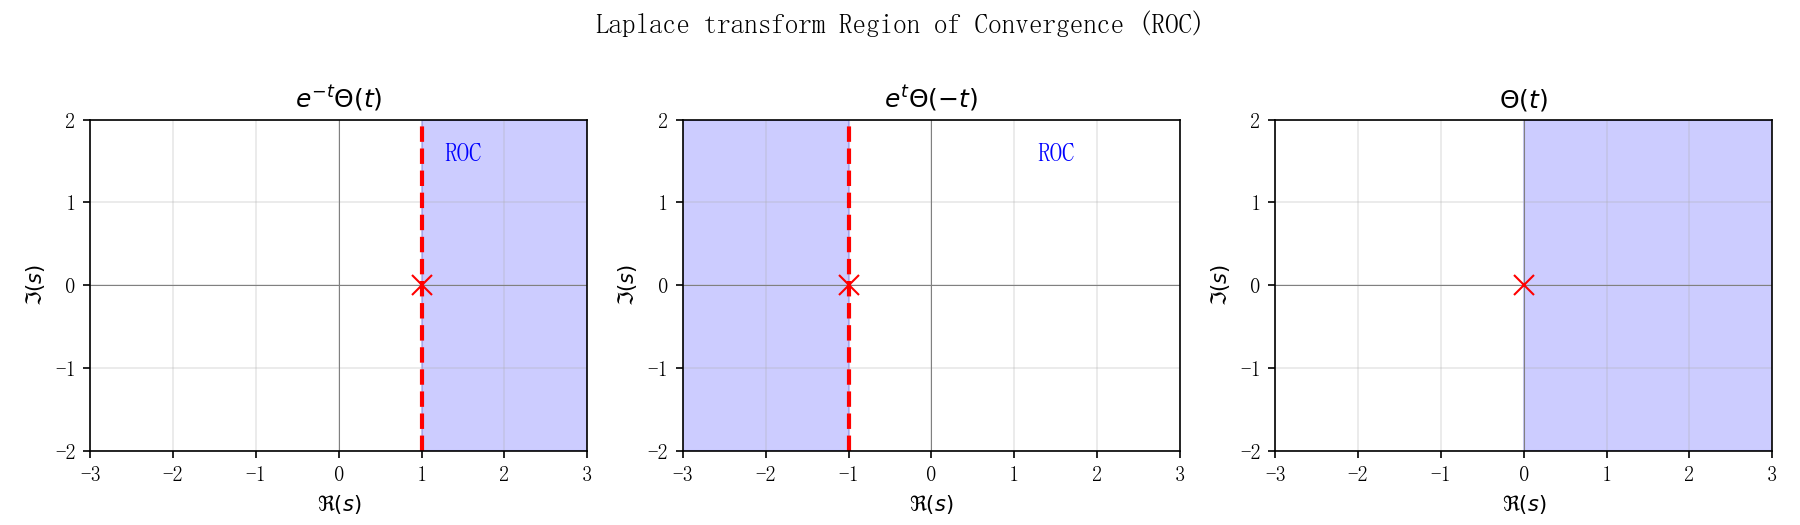
\includegraphics[width=0.85\textwidth]{figures/fig3_4_laplace_roc.png}
\caption{拉普拉斯变换的收敛域 (ROC)。左：$e^{-t}\Theta(t)$ 的 ROC 为 $\Re(s) > -1$；中：$e^{t}\Theta(-t)$（左信号）的 ROC 为 $\Re(s) < 1$；右：$\Theta(t)$ 的 ROC 为 $\Re(s) > 0$。}
\label{fig:laplace_roc}
\end{figure}

\section{拉普拉斯变换的物理应用}
\label{sec:laplace_physics}

\subsection{电路的复频域分析}

\textbf{阻抗法：} 在 $s$ 域中，电感 $L$ 的阻抗为 $sL$，电容 $C$ 的阻抗为 $1/(sC)$，电阻 $R$ 的阻抗为 $R$。这与相量法中的 $\mathrm{i}\omega L$, $1/(\mathrm{i}\omega C)$ 形式一致，但 $s$ 域方法可以处理非正弦激励和初始条件。

\textbf{传递函数：} 系统的输出-输入比 $H(s) = Y(s)/X(s)$ 称为\textbf{传递函数}。它是系统的频域指纹，完全刻画了系统的线性响应特性。
\begin{itemize}
\item 系统的稳定性等价于 $H(s)$ 的所有极点具有负实部。
\item 单位冲激响应 $h(t) = \mathcal{L}^{-1}[H(s)]$。
\item 阶跃响应 $s(t) = \mathcal{L}^{-1}[H(s)/s]$。
\end{itemize}

\begin{example}[完整算例：RLC 电路的阶跃响应]
设串联 RLC 电路初始电流为零，电容初始电压为零。在 $t=0$ 时施加阶跃电压 $V_0\Theta(t)$。

\textbf{步骤 1：写出复频域阻抗。}
$Z(s) = sL + R + 1/(sC)$。

\textbf{步骤 2：电流的拉普拉斯变换。}
\begin{align*}
I(s) &= \frac{V_0/s}{Z(s)} = \frac{V_0}{s(sL + R + 1/(sC))} \\
&= V_0\frac{C}{s^2 LC + sRC + 1}
= \frac{V_0/L}{s^2 + (R/L)s + 1/(LC)}.
\end{align*}

\textbf{步骤 3：引入标准参数。}
令 $\alpha = R/(2L)$（衰减系数），$\omega_0 = 1/\sqrt{LC}$（谐振频率）。
则 $I(s) = \frac{V_0/L}{s^2 + 2\alpha s + \omega_0^2}$。

\textbf{步骤 4：分情况逆变换。}

\underline{欠阻尼 ($\alpha<\omega_0$)：}
令 $\omega_d = \sqrt{\omega_0^2 - \alpha^2}$（阻尼谐振频率）。
\begin{align*}
I(s) &= \frac{V_0/L}{(s+\alpha)^2 + \omega_d^2}, \\
i(t) &= \frac{V_0}{\omega_d L}e^{-\alpha t}\sin(\omega_d t)\,\Theta(t).
\end{align*}

\underline{临界阻尼 ($\alpha=\omega_0$)：}
$I(s) = \frac{V_0/L}{(s+\alpha)^2}$，
$i(t) = \frac{V_0}{L}t e^{-\alpha t}\Theta(t)$。

\underline{过阻尼 ($\alpha>\omega_0$)：}
令 $\beta_{1,2} = \alpha \pm \sqrt{\alpha^2 - \omega_0^2}$。
\begin{align*}
I(s) &= \frac{V_0/L}{(s+\beta_1)(s+\beta_2)}, \\
i(t) &= \frac{V_0}{L(\beta_1-\beta_2)}\left(e^{-\beta_2 t} - e^{-\beta_1 t}\right)\Theta(t).
\end{align*}

拉普拉斯变换将二阶微分方程的初值问题化为代数方程求解，再通过逆变换返回时域。这是求解线性系统的标准方法。
\end{example}

\subsection{传递函数与稳定性分析}

传递函数 $H(s)$ 的极点位置决定系统稳定性：
\begin{itemize}
\item 所有极点在左半平面 $\to$ 稳定（瞬态解指数衰减）。
\item 任何极点在右半平面 $\to$ 不稳定（瞬态解指数增长）。
\item 极点在虚轴上（单根）$\to$ 临界稳定（无阻尼振荡）。
\end{itemize}

\textbf{伯德图 (Bode plot)} 是传递函数 $H(\mathrm{i}\omega)$ 的幅频和相频曲线，采用对数坐标。它直观显示了系统对不同频率输入的响应特性。

\begin{example}[一阶低通滤波器的伯德图]
$H(s) = \frac{1}{1 + sRC}$。

幅频响应（dB）：
\begin{equation}
|H(\mathrm{i}\omega)|_{\text{dB}} = -10\log_{10}\left[1 + (\omega RC)^2\right].
\end{equation}
\begin{itemize}
\item $\omega \ll 1/(RC)$：$|H|_{\text{dB}} \approx 0$ dB（通带）。
\item $\omega \gg 1/(RC)$：$|H|_{\text{dB}} \approx -20\log_{10}(\omega RC)$ dB/十倍频（阻带，斜率 $-20$ dB/dec）。
\item $\omega = 1/(RC)$（截止频率）：$|H|_{\text{dB}} = -3$ dB。
\end{itemize}

相频响应：
\begin{equation}
\angle H(\mathrm{i}\omega) = -\arctan(\omega RC).
\end{equation}
在截止频率处，相位滞后 $45^\circ$。
\end{example}

\subsection{力学系统的类比}

机械振动系统（质量-弹簧-阻尼）与 RLC 电路通过拉普拉斯变换展示出完美的\textbf{力-电类比}：
\begin{equation}
\text{力学：}\quad M s^2 + B s + K \quad\longleftrightarrow\quad
\text{电路：}\quad L s^2 + R s + \frac{1}{C}.
\end{equation}

\begin{table}[h]
\centering
\caption{力-电类比}
\label{tab:mech_elect_analogy}
\begin{tabular}{c|c}
\toprule
力学系统 & 电路系统 \\
\midrule
质量 $M$ & 电感 $L$ \\
阻尼系数 $B$ & 电阻 $R$ \\
劲度系数 $K$ & 倒数电容 $1/C$ \\
力 $F$ & 电压 $V$ \\
速度 $v$ & 电流 $I$ \\
动量 $p$ & 磁通 $\Phi$ \\
\bottomrule
\end{tabular}
\end{table}

\begin{insight}
力-电类比不是肤浅的形式相似，而是源于相同的数学模型。任何一个二阶线性系统——不论是机械的、电气的、声学的还是热学的——都可以用传递函数统一处理。这种 \textbf{跨领域统一性} 是物理学家追求的最高境界。拉普拉斯变换通过揭示不同物理系统中相同的数学结构，实现了这种统一。
\end{insight}

\subsection{偏微分方程中的应用}

考虑半无限长杆的热传导方程：
\begin{equation}
\frac{\partial u}{\partial t} = \kappa \frac{\partial^2 u}{\partial x^2},\quad
x>0,\; t>0,
\end{equation}
初始条件 $u(x,0)=0$，边界条件 $u(0,t)=u_0$，$u(\infty,t)=0$。

对 $t$ 做拉普拉斯变换，偏微分方程化为常微分方程：
\begin{equation}
sU(x,s) = \kappa \frac{\dd^2 U}{\dd x^2}.
\end{equation}

解得 $U(x,s) = C(s)e^{-x\sqrt{s/\kappa}}$。代入边界条件得 $C(s) = u_0/s$，于是
\begin{equation}
U(x,s) = \frac{u_0}{s}e^{-x\sqrt{s/\kappa}}.
\end{equation}

查逆变换表或利用留数定理：
\begin{equation}
u(x,t) = u_0\,\mathrm{erfc}\!\left(\frac{x}{2\sqrt{\kappa t}}\right),
\quad \mathrm{erfc}(z) = \frac{2}{\sqrt{\pi}}\int_z^{\infty} e^{-\eta^2}\,\dd\eta.
\label{eq:heat_laplace_sol}
\end{equation}

\textbf{物理信息：} 温度扰动传播的大致距离为 $\sqrt{\kappa t}$——这正是扩散长度。拉普拉斯变换如此自然地给出了这个重要标度律。

\section*{拉普拉斯变换表}

\begin{table}[h]
\centering
\caption{常用拉普拉斯变换对}
\label{tab:laplace_table}
\begin{tabular}{c|c}
\toprule
$f(t)$ ($t\geq0$) & $F(s) = \mathcal{L}[f]$ \\
\midrule
$\delta(t)$ & $1$ \\
$\Theta(t)$ & $1/s$ \\
$t$ & $1/s^2$ \\
$t^n$ & $n!/s^{n+1}$ \\
$e^{at}$ & $1/(s-a)$ \\
$\sin(\omega_0 t)$ & $\omega_0/(s^2+\omega_0^2)$ \\
$\cos(\omega_0 t)$ & $s/(s^2+\omega_0^2)$ \\
$e^{at}\sin(\omega_0 t)$ & $\omega_0/[(s-a)^2+\omega_0^2]$ \\
$e^{at}\cos(\omega_0 t)$ & $(s-a)/[(s-a)^2+\omega_0^2]$ \\
$t e^{at}$ & $1/(s-a)^2$ \\
$t^n e^{at}$ & $n!/(s-a)^{n+1}$ \\
$\sinh(at)$ & $a/(s^2-a^2)$ \\
$\cosh(at)$ & $s/(s^2-a^2)$ \\
\bottomrule
\end{tabular}
\end{table}

\section{傅里叶变换与拉普拉斯变换的比较}

\begin{table}[h]
\centering
\caption{傅里叶变换与拉普拉斯变换对比}
\label{tab:ft_vs_lt}
\begin{tabular}{c|c}
\toprule
傅里叶变换 & 拉普拉斯变换 \\
\midrule
$s = \mathrm{i}\omega$（纯虚频率） & $s = \sigma + \mathrm{i}\omega$（复频率） \\
双侧变换（$-\infty\to\infty$） & 单侧变换（$0\to\infty$） \\
需要绝对可积条件 & 收敛域更广 \\
稳态分析 & 暂态+稳态 \\
频谱分析 & 传递函数与稳定性 \\
不能处理初始条件 & 自然包含初始条件 \\
\bottomrule
\end{tabular}
\end{table}

\textbf{选择指南：}
\begin{itemize}
\item 分析稳态周期信号、频谱结构、光学衍射 $\to$ 傅里叶变换。
\item 求解初值问题、暂态响应、系统稳定性 $\to$ 拉普拉斯变换。
\item 两者通过 $s = \sigma + \mathrm{i}\omega$ 相联系：傅里叶变换是拉普拉斯变换在虚轴上的特例（当 ROC 包含虚轴时）。
\end{itemize}

\section{本章小结}

\begin{itemize}
\item \textbf{傅里叶级数} 将周期函数分解为离散谐波，是频域分析的起点。
\item \textbf{傅里叶变换} 将时域与频域通过积分变换精确对应，揭示了时频对偶性。
\item \textbf{傅里叶变换的卷积定理} 表明时域卷积对应于频域乘法，这是线性系统分析的基石。
\item \textbf{采样定理} 给出了数字信号处理中采样率的理论下限。
\item \textbf{拉普拉斯变换} 推广了傅里叶变换，通过复频率 $s$ 处理更广泛的函数和初始条件。
\item \textbf{传递函数} 是系统的频域特征函数，稳定性由极点位置决定。
\item \textbf{两个变换统一} 了力学、电学、热学、光学中的线性分析。
\end{itemize}

\subsection*{概念图谱}

\begin{center}
\fbox{\parbox{0.92\textwidth}{
\textbf{积分变换的概念网络：}\\[3pt]
$\bullet$ 周期信号 $\to$ 傅里叶级数（三角形式 $\leftrightarrow$ 复数形式）\\[3pt]
$\bullet$ 傅里叶级数 $\xrightarrow{T\to\infty}$ 傅里叶变换 $\to$ 频谱分析 / 衍射 / 量子力学\\[3pt]
$\bullet$ 卷积定理 $\to$ 线性系统：输出 = 输入 $*$ 冲激响应\\[3pt]
$\bullet$ 采样定理 $\to$ 数字信号处理的基础\\[3pt]
$\bullet$ 傅里叶变换 $\xrightarrow{\text{收敛因子}}$ 拉普拉斯变换 $\to$ ODE/PDE 求解\\[3pt]
$\bullet$ 传递函数 $H(s)$ $\to$ 稳定性分析 / 伯德图 / 滤波器设计\\[3pt]
$\bullet$ Kramers-Kronig 关系：因果性 + 解析性的物理推论
}}
\end{center}

\subsection*{公式参考表}

\begin{table}[h]
\centering
\caption{积分变换核心公式速查}
\label{tab:transform_formulas}
\begin{tabular}{c|c}
\toprule
公式 & 说明 \\
\midrule
$c_n = \frac{1}{T}\int_{-T/2}^{T/2} f(t)e^{-\mathrm{i}n\omega_0 t}\,\dd t$ & 傅里叶级数系数 \\
$\tilde{f}(\omega) = \int_{-\infty}^{\infty} f(t)e^{-\mathrm{i}\omega t}\,\dd t$ & 傅里叶正变换 \\
$f(t) = \frac{1}{2\pi}\int_{-\infty}^{\infty} \tilde{f}(\omega)e^{\mathrm{i}\omega t}\,\dd\omega$ & 傅里叶逆变换 \\
$\mathcal{F}[f'(t)] = \mathrm{i}\omega\tilde{f}(\omega)$ & FT 时域微分 \\
$\mathcal{F}[(f*g)(t)] = \tilde{f}(\omega)\tilde{g}(\omega)$ & FT 卷积定理 \\
$\Delta t\,\Delta\omega \geq 1/2$ & 时宽-带宽积 \\
$F(s) = \int_0^{\infty} f(t)e^{-st}\,\dd t$ & 拉普拉斯变换 \\
$\mathcal{L}[f'(t)] = sF(s) - f(0^-)$ & LT 时域微分 \\
$\mathcal{L}[(f*g)(t)] = F(s)G(s)$ & LT 卷积定理 \\
$f(t) = \frac{1}{2\pi\mathrm{i}}\int_{\sigma_0-\mathrm{i}\infty}^{\sigma_0+\mathrm{i}\infty} F(s)e^{st}\,\dd s$ & 拉普拉斯逆变换 \\
\bottomrule
\end{tabular}
\end{table}

\section*{习题}

\textbf{基础题（巩固概念）}

\begin{enumerate}
\item 求周期为 $2\pi$ 的方波 $f(t) = \mathrm{sgn}(\sin t)$ 的傅里叶级数展开（三角形式和复数形式）。
\item 证明傅里叶变换的时移性质：若 $\tilde{f}(\omega) = \mathcal{F}[f(t)]$，则 $\mathcal{F}[f(t-t_0)] = e^{-\mathrm{i}\omega t_0}\tilde{f}(\omega)$。
\item 计算 $\mathcal{F}[e^{-a|t|}]$（$a>0$），并验证帕塞瓦尔定理。
\item 求 $\mathcal{L}[\sin(\omega_0 t)\Theta(t)]$ 和 $\mathcal{L}[\cos(\omega_0 t)\Theta(t)]$。
\item 求矩形脉冲 $p_T(t)$ 的傅里叶变换，并画出 $T=1$ 和 $T=2$ 时的幅度谱 $|\tilde{p}_T(\omega)|$。
\item 求 $\mathcal{L}[t^2 e^{-3t}\Theta(t)]$。
\end{enumerate}

\textbf{提高题（应用分析）}

\begin{enumerate}
\item[7.] 利用傅里叶变换求解一维无限长弦的波动方程 $u_{tt} = c^2 u_{xx}$，初始条件 $u(x,0)=\phi(x)$，$u_t(x,0)=0$。\textbf{提示：} 对 $x$ 做傅里叶变换，求解关于 $t$ 的 ODE，然后逆变换。
\item[8.] 求传递函数 $H(s) = \frac{1}{(s+1)(s+2)}$ 的单位冲激响应和单位阶跃响应。
\item[9.] 用拉普拉斯变换求解 $LC$ 串联电路的零状态响应（施加 $V_0\sin(\omega t)$ 电压）。讨论 $\omega = \omega_0 = 1/\sqrt{LC}$ 时的共振情形。
\item[10.] 求 $f(t) = t^n\Theta(t)$ 的拉普拉斯变换，验证 $\mathcal{L}[t^n] = n!/s^{n+1}$。
\item[11.] 一个二阶低通滤波器 $H(s) = \frac{\omega_0^2}{s^2 + 2\alpha s + \omega_0^2}$。讨论 $\alpha=0$（无阻尼）、$\alpha<\omega_0$（欠阻尼）、$\alpha=\omega_0$（临界阻尼）时的单位阶跃响应，并画出 $h(t)$ 的波形。
\item[12.] 求 $f(t) = \cos(100\pi t)$ 的傅里叶变换。如果以 $f_s=120$ Hz 采样，解释为什么会出现混叠（aliasing）现象。
\end{enumerate}

\textbf{挑战题（综合拓展）}

\begin{enumerate}
\item[13.]（因果性与解析性）因果信号 $f(t)=\Theta(t)\sin(\omega_0 t)e^{-\alpha t}$ 的傅里叶变换是什么？它与拉普拉斯变换有何关系？验证当 $\alpha\to0^+$ 时结果趋近于正弦函数的变换。
\item[14.]（采样定理的证明）设 $f(t)$ 的傅里叶变换在 $|\omega|>\Omega$ 时为零（带限信号）。证明采样定理：$f(t) = \sum_{n=-\infty}^{\infty} f(n\pi/\Omega)\,\mathrm{sinc}(\Omega t - n\pi)$。
\item[15.]（热传导方程的 Laplace 解）用拉普拉斯变换求解有限长杆 $0<x<L$ 的热传导方程，两端温度 $u(0,t)=u(L,t)=0$，初始温度 $u(x,0)=T_0$。对比分离变量法的结果。
\item[16.]（调制与解调）信号 $m(t)$ 被载波 $\cos(\omega_c t)$ 调制为 $f(t)=m(t)\cos(\omega_c t)$。用傅里叶变换解释如何通过低通滤波器从 $f(t)$ 恢复 $m(t)$。
\item[17.]（希尔伯特变换）证明解析信号 $f_a(t) = f(t) + \mathrm{i}\hat{f}(t)$ 的傅里叶变换 $\tilde{f}_a(\omega)$ 在 $\omega<0$ 时为零。利用这个性质解释如何从实信号构造其复包络。
\item[18.]（分数阶傅里叶变换）分数阶傅里叶变换 $F^{\alpha}[f]$ 是传统 FT 的推广。说明当 $\alpha=0$ 时就是恒等变换，$\alpha=\pi/2$ 时是标准傅里叶变换，$\alpha=\pi$ 时是时间反转。讨论其在量子力学中的 chirp 信号分析中的应用。
\end{enumerate}

% ============================================================
%  第 4 章  偏微分方程与特殊函数（扩展版）
% ============================================================

\chapter{偏微分方程与特殊函数}

\section{本章概览与学习路线}

牛顿第二定律 $\mathbf{F}=m\mathbf{a}$ 是常微分方程——描述的是单个质点的运动。但在连续介质（流体、弹性体、电磁场、量子波函数）中，物理量不仅是时间的函数，也是空间的函数。这就需要 \textbf{偏微分方程 (Partial Differential Equations, PDEs)}。

特殊函数不是数学家臆造的玩具，而是物理对称性在求解 PDE 过程中不可回避的产物——球对称 $\to$ 勒让德多项式，柱对称 $\to$ 贝塞尔函数，谐振子 $\to$ 埃尔米特多项式，氢原子 $\to$ 拉盖尔多项式。

\begin{center}
\fbox{\parbox{0.9\textwidth}{\centering
\textbf{核心逻辑链条：}\\
物理问题 $\to$ 三大 PDE 分类 $\to$ 对称性引导坐标系选择 $\to$ 分离变量 \\
$\to$ 本征值问题 $\to$ 特殊函数自然涌现 $\to$ SL 理论统一框架
}}
\end{center}

\subsection*{不同读者的学习路径}

\begin{itemize}
\item \textbf{物理专业学生：} 重点关注 \S4.2（三大 PDE 的物理含义）、\S4.3（分离变量法——量子力学和电磁学的基础）、\S4.4--\S4.5（勒让德和贝塞尔函数——原子物理和电磁散射的基础）。
\item \textbf{数学学生：} 重点关注 \S4.3（分离变量法的严格推导）、\S4.7（SL 理论的形式化框架）、\S4.8（球贝塞尔函数与散射理论）。
\item \textbf{工程学生：} 重点关注 \S4.2（三类 PDE 的判别与边界条件），\S4.3（分离变量法的算例），\S4.4--\S4.5（正交函数系的工程应用）。
\end{itemize}

\section{三大经典偏微分方程}
\label{sec:pde_types}

\subsection*{动机：物理学家只有这三类 PDE？}

几乎所有的物理定律都可以归入这三类：波动（信息传播）、扩散（信息模糊化）、稳态（场的静态平衡）。它们的区别不在于推导来源，而在于\textbf{特征线的结构}——也就是信息的传播方式。

\subsection{波动方程——双曲型}

\textbf{一维形式：}
\begin{equation}
\frac{\partial^2 u}{\partial t^2} = c^2 \frac{\partial^2 u}{\partial x^2},
\label{eq:wave1d}
\end{equation}
其中 $c$ 是波速。

\textbf{物理背景：} 弦的微小横振动中，张力 $T$ 和线密度 $\rho$ 决定了 $c = \sqrt{T/\rho}$。电磁波中 $c = 1/\sqrt{\mu_0\varepsilon_0}$。

\textbf{达朗贝尔解：} 对一维无界波动方程，通解为
\begin{equation}
u(x,t) = f(x-ct) + g(x+ct),
\end{equation}
即左右行波的叠加。

\textbf{达朗贝尔公式的推导：} 作变量代换 $\xi = x - ct$, $\eta = x + ct$，则波动方程化为 $\partial^2 u/\partial\xi\partial\eta = 0$。对 $\xi$ 积分得 $\partial u/\partial\eta = h(\eta)$，再对 $\eta$ 积分得 $u = \int h(\eta)\,\dd\eta + f(\xi) = f(\xi) + g(\eta)$。

\textbf{物理分类：}
\begin{itemize}
\item \textbf{双曲型}：信息以有限速度传播（特征线为 $x\pm ct = \text{常数}$）。
\item 初值问题的解由初始位移和初始速度唯一确定。
\item 能量守恒：机械能 $\int (\frac12 u_t^2 + \frac12 c^2 u_x^2)\,\dd x$ 不随时间变化。
\end{itemize}

\begin{insight}[双曲型方程的物理直觉]
双曲型 PDE 的核心特征是\textbf{有限传播速度}。这一点在狭义相对论中至关重要：如果信息可以超光速传播，因果律将被破坏。波动方程的特征线 $x \pm ct = \text{常数}$ 正是光锥在 $1+1$ 维时空中的投影。
\end{insight}

\subsection{热传导方程——抛物型}

\textbf{形式：}
\begin{equation}
\frac{\partial u}{\partial t} = \kappa \nabla^2 u.
\label{eq:heat}
\end{equation}

\textbf{物理背景：} $\kappa$ 是热扩散率。傅里叶热传导定律 $\mathbf{q} = -k\nabla T$（热流正比于温度梯度）结合能量守恒导出此方程。

\textbf{物理分类：}
\begin{itemize}
\item \textbf{抛物型}：信息以无限速度传播（解在 $t>0$ 后立即处处非零——但实际有意义的部分在扩散长度 $\sqrt{\kappa t}$ 内）。
\item 解是无限可微的（即使初始条件有间断，$t>0$ 后立刻光滑化）。
\item 熵增：温度梯度自发衰减，趋于均匀。
\end{itemize}

\begin{insight}[抛物型方程的物理直觉]
热传导方程展现了"时间之箭"：将 $t\to -t$ 替换，方程变为 $u_t = -\kappa u_{xx}$，这是向后热传导方程——物理上不可能，因为它需要从均匀温度场恢复初始的不均匀性。这正是\textbf{热力学第二定律}在 PDE 层面的体现。
\end{insight}

\subsection{泊松方程与拉普拉斯方程——椭圆型}

\textbf{形式：}
\begin{equation}
\nabla^2 u = -\frac{\rho}{\varepsilon_0}\quad\text{(泊松)},\qquad
\nabla^2 u = 0\quad\text{(拉普拉斯)}.
\label{eq:poisson_laplace}
\end{equation}

\textbf{物理分类：}
\begin{itemize}
\item \textbf{椭圆型}：稳态问题，不涉及时间演化。
\item 解由边界条件唯一确定（Dirichlet 或 Neumann 条件）。
\item 解具有"刚性"：最大值原理（调和函数的最大值必在边界上）。
\end{itemize}

\begin{theorem}[最大值原理]
若 $\nabla^2 u = 0$ 在有界区域 $\Omega$ 内成立且 $u\in C^2(\Omega)\cap C^0(\bar\Omega)$，则 $u$ 的最大值和最小值均在边界 $\partial\Omega$ 上达到。
\end{theorem}

最大值原理的物理意义：稳态热场中，内部任意点的温度不可能高于边界最高温度——否则热量会从内部流向边界，就不是稳态了。

% 三类 PDE 示意图
\begin{figure}[H]
\centering
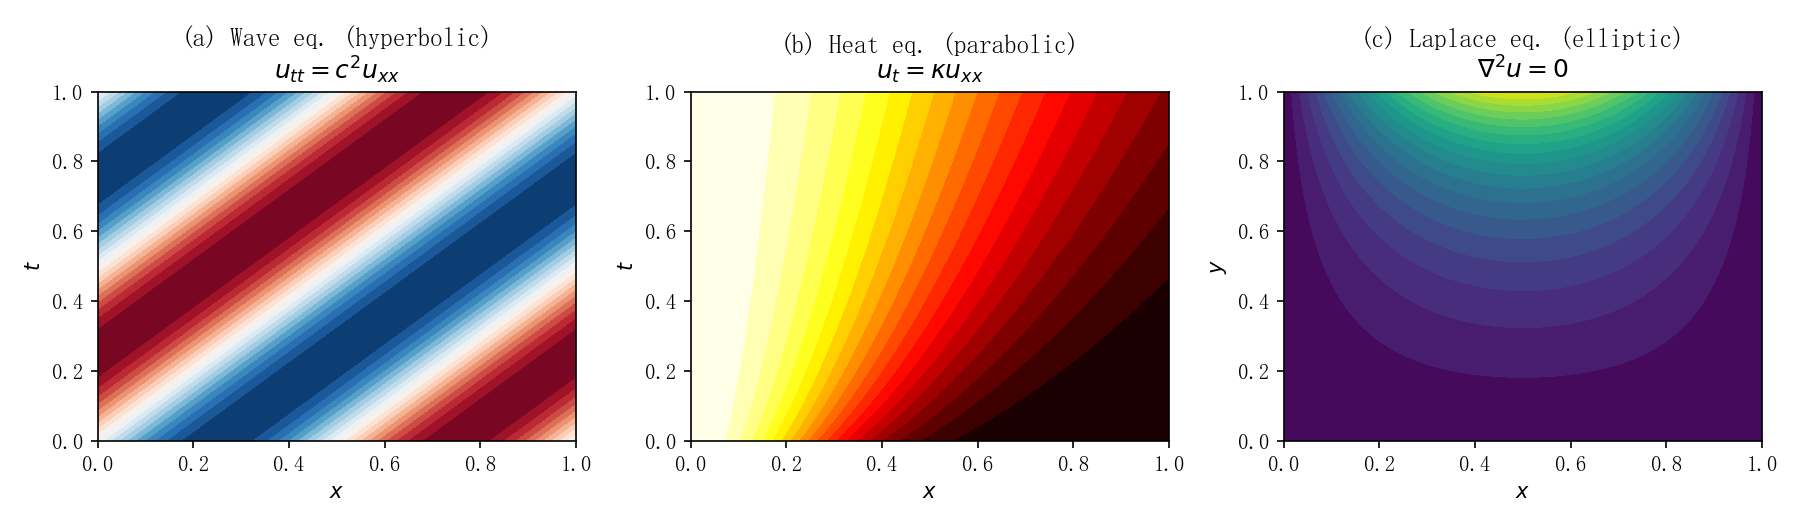
\includegraphics[width=0.85\textwidth]{figures/fig4_1_pde_types.png}
\caption{三类 PDE 的数值解示意图：(a) 波动方程（双曲型）——沿特征线传播的等相位线；(b) 热传导方程（抛物型）——温度扩散，前沿随 $\sqrt{t}$ 推进；(c) 拉普拉斯方程（椭圆型）——稳态分布，由边界条件唯一决定。}
\label{fig:pde_types}
\end{figure}

\subsection{PDE 的分类统一}

一般二阶线性 PDE 写为：
\begin{equation}
A\frac{\partial^2 u}{\partial x^2} + 2B\frac{\partial^2 u}{\partial x\partial y}
+ C\frac{\partial^2 u}{\partial y^2} + \text{(低阶项)} = 0.
\end{equation}

分类由判别式 $\Delta = B^2 - AC$ 决定：
\begin{itemize}
\item $\Delta > 0$：\textbf{双曲型}（波动方程），两条实特征线。
\item $\Delta = 0$：\textbf{抛物型}（热传导方程），一条实特征线。
\item $\Delta < 0$：\textbf{椭圆型}（拉普拉斯方程），无实特征线。
\end{itemize}

这个分类名称来源于二次型 $A\xi^2 + 2B\xi\eta + C\eta^2$ 的几何类型，与圆锥曲线的分类完全一致。

\begin{example}[PDE 分类练习]
判断下列方程的类型：

\textbf{(1)} $u_{xx} + 2u_{xy} + u_{yy} = 0$：$A=1,B=1,C=1$，$\Delta = 1-1 = 0$，抛物型。

\textbf{(2)} $u_{xx} - 3u_{yy} = 0$：$A=1,B=0,C=-3$，$\Delta = 0-(-3) = 3 > 0$，双曲型。

\textbf{(3)} $u_{xx} + u_{yy} + u_{zz} = 0$：三维拉普拉斯方程，椭圆型。

\textbf{(4)} $u_t = u_{xx} + u_{yy}$：二维热传导方程，抛物型（对 $t$ 一阶、对 $x,y$ 二阶）。
\end{example}

\section{分离变量法}
\label{sec:separation}

\subsection*{动机：如何把 PDE 拆成 ODE？}

分离变量法的核心想法很直接：假设 $u(x,t)=X(x)T(t)$，代入 PDE 后，等号两边分别是 $x$ 的函数和 $t$ 的函数。要使它们对所有 $x,t$ 都相等，只有一种可能：两边都等于同一个常数。这个常数就是\textbf{分离常数}，它将在后续步骤中引出本征值问题。

\subsection{一般步骤}

分离变量法的标准流程：

\begin{enumerate}
\item \textbf{假设分离变量形式} $u(x,t) = X(x)T(t)$（或 $u(x,y) = X(x)Y(y)$ 等）。
\item \textbf{代入 PDE 并分离}，得到两个（或更多）常微分方程和一个分离常数。
\item \textbf{求解本征值问题}——空间 ODE + 齐次边界条件给出本征值和本征函数。
\item \textbf{求解时间 ODE}——每个本征值对应一个时间演化模式。
\item \textbf{叠加所有模式}，由非齐次初始条件通过正交性确定展开系数。
\end{enumerate}

\subsection{一维波动方程（两端固定弦）}

\begin{align}
\frac{\partial^2 u}{\partial t^2} &= c^2 \frac{\partial^2 u}{\partial x^2},\quad
0<x<L,\\
u(0,t) &= u(L,t) = 0,\\
u(x,0) &= f(x),\quad u_t(x,0) = g(x).
\end{align}

\textbf{第一步：设 $u(x,t) = X(x)T(t)$，代入得}
\begin{equation}
X T'' = c^2 X'' T \quad\Longrightarrow\quad
\frac{T''}{c^2 T} = \frac{X''}{X} = -\lambda.
\end{equation}

\textbf{第二步：求解空间 ODE（本征值问题）}
\begin{equation}
X'' + \lambda X = 0,\quad X(0)=X(L)=0.
\end{equation}

本征值和本征函数：
\begin{equation}
\lambda_n = \left(\frac{n\pi}{L}\right)^2,\quad
X_n(x) = \sin\frac{n\pi x}{L},\quad n=1,2,3,\dots
\label{eq:wave_eigen}
\end{equation}

\textbf{第三步：求解时间 ODE}
\begin{equation}
T''_n + c^2\lambda_n T_n = 0 \quad\Longrightarrow\quad
T_n(t) = A_n\cos(\omega_n t) + B_n\sin(\omega_n t),
\end{equation}
其中 $\omega_n = n\pi c/L$ 是第 $n$ 阶固有频率。

\textbf{第四步：叠加并利用初始条件确定系数}
\begin{align}
u(x,t) &= \sum_{n=1}^{\infty} \sin\frac{n\pi x}{L}
\left[A_n\cos(\omega_n t) + B_n\sin(\omega_n t)\right],\\
A_n &= \frac{2}{L}\int_0^L f(x)\sin\frac{n\pi x}{L}\,\dd x,\\
B_n &= \frac{2}{n\pi c}\int_0^L g(x)\sin\frac{n\pi x}{L}\,\dd x.
\end{align}

\begin{insight}
本征函数 $\sin(n\pi x/L)$ 正是傅里叶正弦级数的基函数。分离变量法在此处自然引出傅里叶级数——不是我们"选择"了正弦函数，而是两端固定的边界条件\textbf{强迫}本征函数必须是正弦函数。这就是物理对称性决定数学形式的绝佳例证。
\end{insight}

\subsection{一维热传导方程——完整算例}

\begin{example}[两端固定温度的杆]
一根长度为 $L$ 的均匀细杆，初始温度分布为 $u(x,0)=T_0\sin(\pi x/L)$，两端温度保持 $u(0,t)=u(L,t)=0$。求温度分布 $u(x,t)$。

\textbf{步骤 1：分离变量。}
设 $u(x,t)=X(x)T(t)$，代入 $u_t = \kappa u_{xx}$：
\begin{equation}
\frac{T'}{\kappa T} = \frac{X''}{X} = -\lambda.
\end{equation}

\textbf{步骤 2：空间 ODE。}
$X'' + \lambda X = 0$，$X(0)=X(L)=0$。
与波动方程相同：$\lambda_n = (n\pi/L)^2$，$X_n(x)=\sin(n\pi x/L)$。

\textbf{步骤 3：时间 ODE。}
$T'_n = -\kappa\lambda_n T_n$，解得 $T_n(t) = C_n e^{-\kappa (n\pi/L)^2 t}$。

\textbf{步骤 4：一般解。}
\begin{equation}
u(x,t) = \sum_{n=1}^{\infty} C_n \sin\frac{n\pi x}{L} e^{-\kappa (n\pi/L)^2 t}.
\end{equation}

\textbf{步骤 5：代入初始条件。}
\begin{equation}
u(x,0) = \sum_{n=1}^{\infty} C_n \sin\frac{n\pi x}{L} = T_0\sin\frac{\pi x}{L}.
\end{equation}
由正弦级数的正交性：$C_1 = T_0$，$C_n=0$（$n\geq2$）。

\textbf{步骤 6：最终解。}
\begin{equation}
\boxed{\;u(x,t) = T_0\sin\frac{\pi x}{L}\, e^{-\kappa(\pi/L)^2 t}\;}.
\end{equation}

\textbf{物理解读：} 温度呈正弦分布，整体指数衰减，衰减时间常数 $\tau = (L/\pi)^2/\kappa$。杆越长，衰减越慢。
\end{example}

\subsection{二维拉普拉斯方程（矩形区域）}

\begin{equation}
\frac{\partial^2 u}{\partial x^2} + \frac{\partial^2 u}{\partial y^2} = 0,\quad
0<x<a,\;0<y<b.
\end{equation}

边界条件：$u(0,y)=u(a,y)=0$，$u(x,0)=0$，$u(x,b)=f(x)$。

分离变量 $u(x,y)=X(x)Y(y)$：
\begin{equation}
\frac{X''}{X} = -\frac{Y''}{Y} = -k^2.
\end{equation}

$X$ 方程的解：$X_n(x) = \sin\frac{n\pi x}{a}$（$n=1,2,\dots$）。
$Y$ 方程：$Y_n'' = k_n^2 Y_n$，$k_n = n\pi/a$。

满足 $Y_n(0)=0$ 的解为 $Y_n(y) = \sinh(k_n y)$。最终解：
\begin{equation}
u(x,y) = \sum_{n=1}^{\infty} c_n \sin\frac{n\pi x}{a}\,
\sinh\frac{n\pi y}{a},
\end{equation}
其中 $c_n$ 由 $u(x,b)=f(x)$ 确定：
\begin{equation}
c_n = \frac{2}{a\sinh(k_n b)}\int_0^a f(x)\sin\frac{n\pi x}{a}\,\dd x.
\end{equation}

\subsection{球对称：三维拉普拉斯方程}

在球坐标中，拉普拉斯方程为：
\begin{equation}
\frac{1}{r^2}\frac{\partial}{\partial r}\left(r^2\frac{\partial u}{\partial r}\right)
+ \frac{1}{r^2\sin\theta}\frac{\partial}{\partial\theta}\left(\sin\theta\frac{\partial u}{\partial\theta}\right)
+ \frac{1}{r^2\sin^2\theta}\frac{\partial^2 u}{\partial\phi^2} = 0.
\end{equation}

分离变量 $u(r,\theta,\phi) = R(r)\Theta(\theta)\Phi(\phi)$ 得到三个 ODE：
\begin{align}
\frac{1}{\Phi}\frac{\dd^2\Phi}{\dd\phi^2} &= -m^2,\\
\frac{1}{\sin\theta}\frac{\dd}{\dd\theta}\left(\sin\theta\frac{\dd\Theta}{\dd\theta}\right)
+ \left[l(l+1) - \frac{m^2}{\sin^2\theta}\right]\Theta &= 0,\\
\frac{1}{r^2}\frac{\dd}{\dd r}\left(r^2\frac{\dd R}{\dd r}\right)
- \frac{l(l+1)}{r^2}R &= 0.
\end{align}

角向方程的解是\textbf{球谐函数} $Y_{lm}(\theta,\phi)$，径向方程的解是 $r^l$ 和 $r^{-(l+1)}$。这正是静电场中多极展开的基础。

\section{勒让德多项式}
\label{sec:legendre}

\subsection*{动机：球对称问题为什么必然出现勒让德多项式？}

在球坐标中分离变量后，$\theta$ 方向的方程（经过变换 $x=\cos\theta$）就是勒让德方程。要求解在 $\theta=0,\pi$（南北极）处有限，$l$ 必须为整数——这就是角动量量子化的数学起源！勒让德多项式不是一个"可以选"的基函数，而是物理约束（有界性）迫使的唯一选择。

\subsection{勒让德方程}

$\theta$ 方程在令 $x = \cos\theta$ 后化为\textbf{勒让德方程} ($m=0$ 时)：
\begin{equation}
(1-x^2)\frac{\dd^2 P}{\dd x^2} - 2x\frac{\dd P}{\dd x}
+ l(l+1)P = 0,\qquad x\in[-1,1].
\label{eq:legendre_ode}
\end{equation}

该方程在 $x=\pm1$ 处具有正则奇点。要求解在 $x=\pm1$ 处有界——即物理上在球轴的南北极温度/势有限——这迫使 $l$ 为非负整数。

\subsection{勒让德多项式}

$l$ 为整数时，勒让德方程的多项式解称为\textbf{勒让德多项式}：
\begin{align}
P_0(x) &= 1,\\
P_1(x) &= x,\\
P_2(x) &= \frac{1}{2}(3x^2-1),\\
P_3(x) &= \frac{1}{2}(5x^3-3x),\\
P_4(x) &= \frac{1}{8}(35x^4-30x^2+3).
\end{align}

\textbf{罗德里格斯公式：}
\begin{equation}
P_l(x) = \frac{1}{2^l l!}\frac{\dd^l}{\dd x^l}(x^2-1)^l.
\label{eq:rodrigues}
\end{equation}

\textbf{递推关系：}
\begin{equation}
(l+1)P_{l+1}(x) = (2l+1)xP_l(x) - lP_{l-1}(x).
\end{equation}
由 $P_0(x)=1$, $P_1(x)=x$ 和递推关系可以生成所有高阶勒让德多项式。

\textbf{正交性：}
\begin{equation}
\int_{-1}^{1} P_l(x)P_{l'}(x)\,\dd x = \frac{2}{2l+1}\delta_{ll'}.
\label{eq:legendre_ortho}
\end{equation}

\textbf{完备性：} $[-1,1]$ 上的任意良函数可以展开为勒让德级数：
\begin{equation}
f(x) = \sum_{l=0}^{\infty} A_l P_l(x),\quad
A_l = \frac{2l+1}{2}\int_{-1}^{1} f(x)P_l(x)\,\dd x.
\end{equation}

% 勒让德多项式图
\begin{figure}[H]
\centering
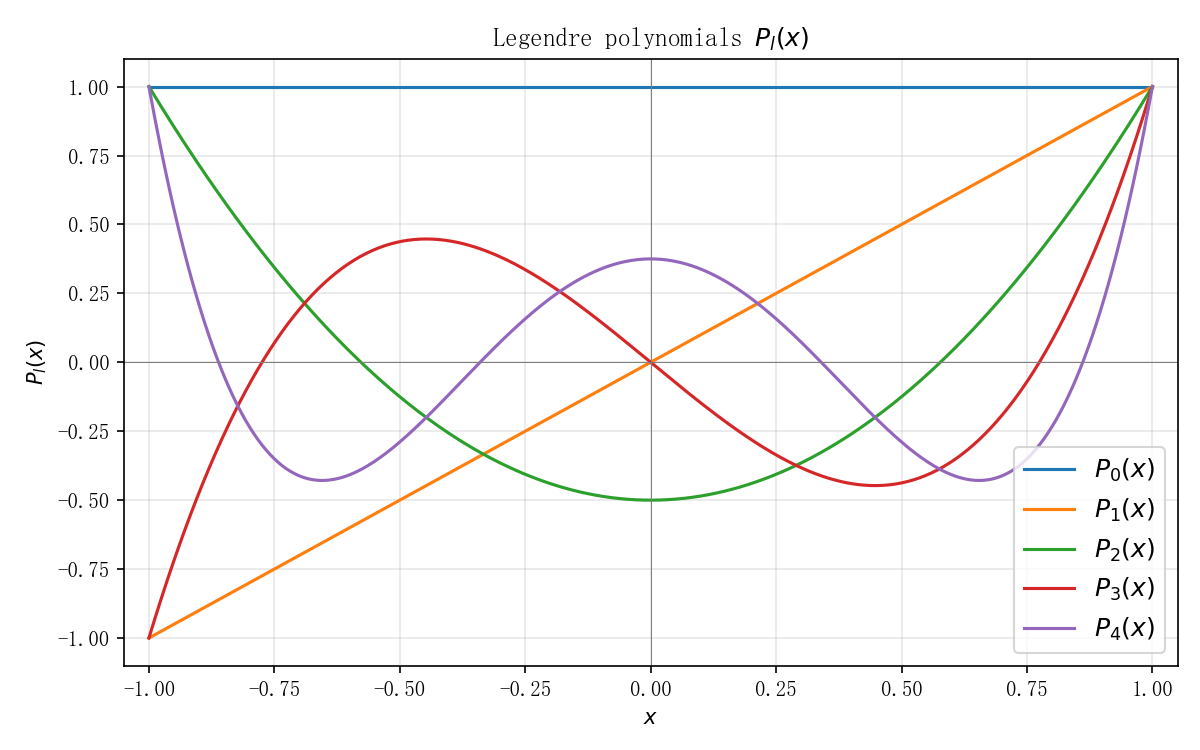
\includegraphics[width=0.6\textwidth]{figures/fig4_2_legendre.png}
\caption{前 5 阶勒让德多项式 $P_l(x)$。注意：$P_l(1)=1$ 对所有 $l$ 成立；$P_l$ 在 $(-1,1)$ 内有 $l$ 个零点。}
\label{fig:legendre}
\end{figure}

\subsection{物理应用：静电场的多极展开}

在远离电荷分布的区域，电势可以按勒让德多项式展开：
\begin{equation}
\phi(r,\theta) = \frac{1}{4\pi\varepsilon_0}\sum_{l=0}^{\infty}
\frac{1}{r^{l+1}}P_l(\cos\theta)\int r'^l P_l(\cos\theta')\rho(\mathbf{r}')\,\dd V'.
\end{equation}

\textbf{前三项：}
\begin{itemize}
\item $l=0$：单极项 $\phi_0 = \dfrac{Q}{4\pi\varepsilon_0 r}$，$Q$ 为总电荷。
\item $l=1$：偶极项 $\phi_1 = \dfrac{\mathbf{p}\cdot\mathbf{r}}{4\pi\varepsilon_0 r^3}$，$\mathbf{p} = \int \mathbf{r}'\rho\,\dd V'$ 为电偶极矩。
\item $l=2$：四极项 $\phi_2 = \dfrac{1}{4\pi\varepsilon_0}\dfrac{1}{2r^5}\sum_{ij} Q_{ij}x_i x_j$，$Q_{ij}$ 为四极矩张量。
\end{itemize}

\begin{insight}
多极展开的物理意义：远场电势由总电荷（单极）主导，当总电荷为零时由偶极主导，以此类推。这如同傅里叶级数在空间角域中的对应——将电荷分布的角向结构分解为不同"空间频率"的成分。实验物理中，通过测量远场多极矩可以反推源分布的对称性——这正是原子核形状和分子结构的诊断工具。
\end{insight}

\subsection{连带勒让德函数与球谐函数}

对于 $m\neq0$ 的情况，方程的解是\textbf{连带勒让德函数}：
\begin{equation}
P_l^m(x) = (1-x^2)^{m/2}\frac{\dd^m}{\dd x^m}P_l(x),\qquad -l\leq m\leq l.
\label{eq:associated_legendre}
\end{equation}

球谐函数为：
\begin{equation}
Y_{lm}(\theta,\phi) = (-1)^m\sqrt{\frac{2l+1}{4\pi}\frac{(l-m)!}{(l+m)!}}
P_l^m(\cos\theta)e^{\mathrm{i}m\phi}.
\label{eq:spherical_harmonic}
\end{equation}

\textbf{正交归一：}
\begin{equation}
\int_0^{2\pi}\int_0^{\pi} Y_{lm}^*(\theta,\phi)Y_{l'm'}(\theta,\phi)\,
\sin\theta\,\dd\theta\,\dd\phi = \delta_{ll'}\delta_{mm'}.
\end{equation}

球谐函数是 $\hat{L}^2$ 和 $\hat{L}_z$ 的共同本征函数，也是 $L^2(S^2)$（二维球面上的平方可积函数空间）的完备正交基。任何球面上的函数（如地磁场分布、CMB 温度图）都可以展开为球谐级数。

% 球谐函数图
\begin{figure}[H]
\centering
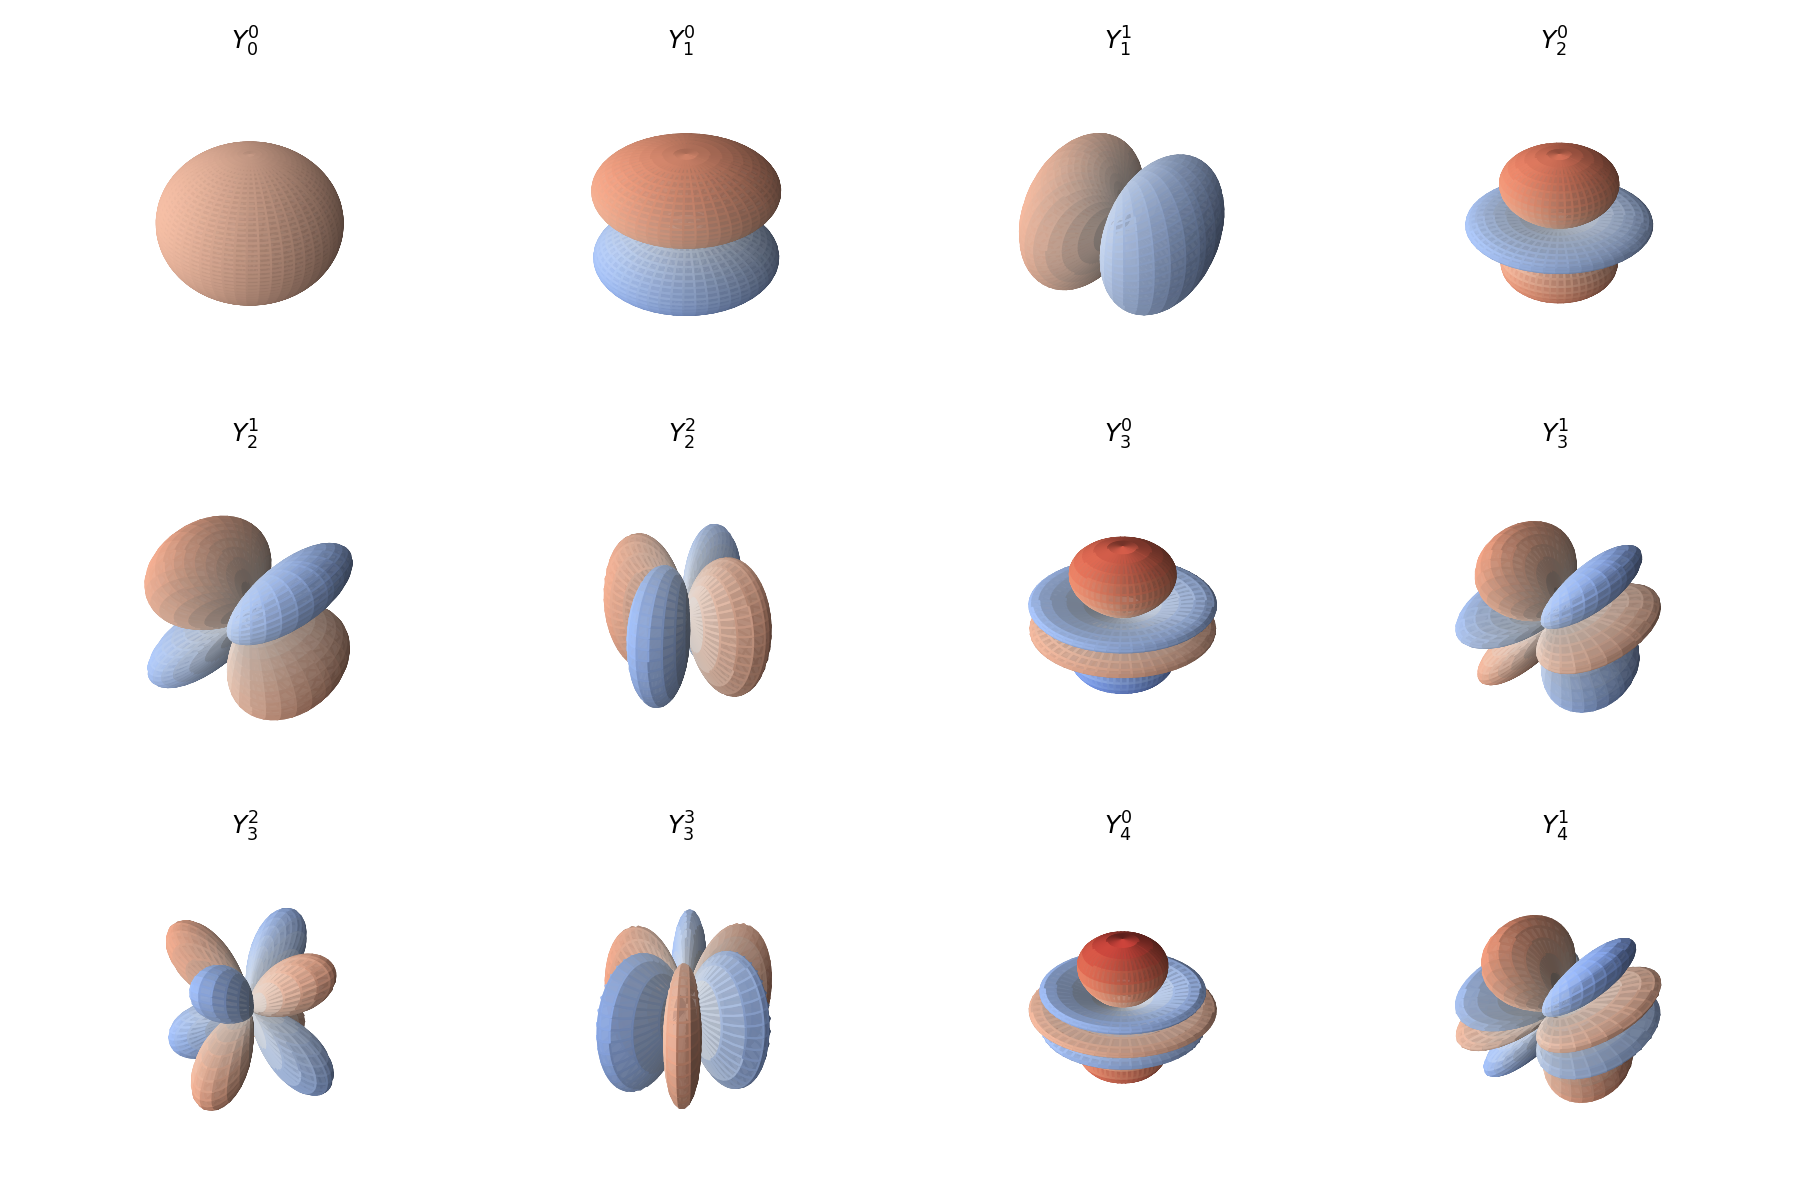
\includegraphics[width=0.85\textwidth]{figures/fig4_5_spherical_harmonics.png}
\caption{球谐函数 $Y_l^m(\theta,\phi)$ 的 3D 可视化。颜色表示实部的正负，径向距离表示 $|Y_l^m|$ 的大小。$l$ 增加意味着角向振荡加快。}
\label{fig:spherical_harmonics}
\end{figure}

\section{贝塞尔函数}
\label{sec:bessel}

\subsection*{动机：柱对称问题为什么产生贝塞尔函数？}

与球对称类似，在柱坐标或极坐标中分离变量后，径向方程变为贝塞尔方程。贝塞尔函数 $J_0(x)$ 描述了圆膜振动、圆柱波导中的电磁场分布、以及热传导中的径向温度分布。它的关键特征是：在 $x=0$ 处有限，在大 $x$ 处像 $\cos(x)/\sqrt{x}$ 衰减——这正是"柱面波"的几何稀释效应。

\subsection{贝塞尔方程}

在柱坐标或极坐标中对拉普拉斯方程、波动方程或热传导方程分离变量时，径向方程通常化为\textbf{贝塞尔方程}：
\begin{equation}
x^2\frac{\dd^2 y}{\dd x^2} + x\frac{\dd y}{\dd x} + (x^2 - \nu^2)y = 0.
\label{eq:bessel_ode}
\end{equation}

其中 $\nu$ 是阶数，由分离变量常数 $m$ 决定。在柱对称问题中，$\nu = m$（整数）。

\subsection{第一类贝塞尔函数}

贝塞尔方程的两个线性无关解是 $J_\nu(x)$ 和 $Y_\nu(x)$（或 $N_\nu(x)$），分别称为\textbf{第一类和第二类贝塞尔函数}。

$J_\nu(x)$ 的级数表示：
\begin{equation}
J_\nu(x) = \sum_{k=0}^{\infty}
\frac{(-1)^k}{k!\,\Gamma(\nu+k+1)}\left(\frac{x}{2}\right)^{\nu+2k}.
\label{eq:bessel_series}
\end{equation}

\textbf{渐近行为：}
\begin{align}
J_\nu(x) &\sim \frac{1}{\Gamma(\nu+1)}\left(\frac{x}{2}\right)^\nu,\quad x\to 0,\\
J_\nu(x) &\sim \sqrt{\frac{2}{\pi x}}\cos\left(x - \frac{\nu\pi}{2} - \frac{\pi}{4}\right),\quad x\to\infty.
\label{eq:bessel_asym}
\end{align}

\textbf{递推关系：}
\begin{align}
J_{\nu-1}(x) + J_{\nu+1}(x) &= \frac{2\nu}{x}J_\nu(x),\\
J_{\nu-1}(x) - J_{\nu+1}(x) &= 2J'_\nu(x).
\end{align}

\begin{insight}
$J_\nu(x)$ 在 $x\to\infty$ 时像衰减的正弦波，这正是"径向波动"的特征：
\begin{itemize}
\item $1/\sqrt{x}$ 衰减：二维或三维波在扩展中的能量稀释。
\item 余弦相位：波从原点径向向外传播。
\end{itemize}
对比之下，勒让德多项式在 $x\in[-1,1]$ 上振荡但幅度恒定——因为它是角向函数，不存在几何扩散效应。
\end{insight}

% 贝塞尔函数图
\begin{figure}[H]
\centering
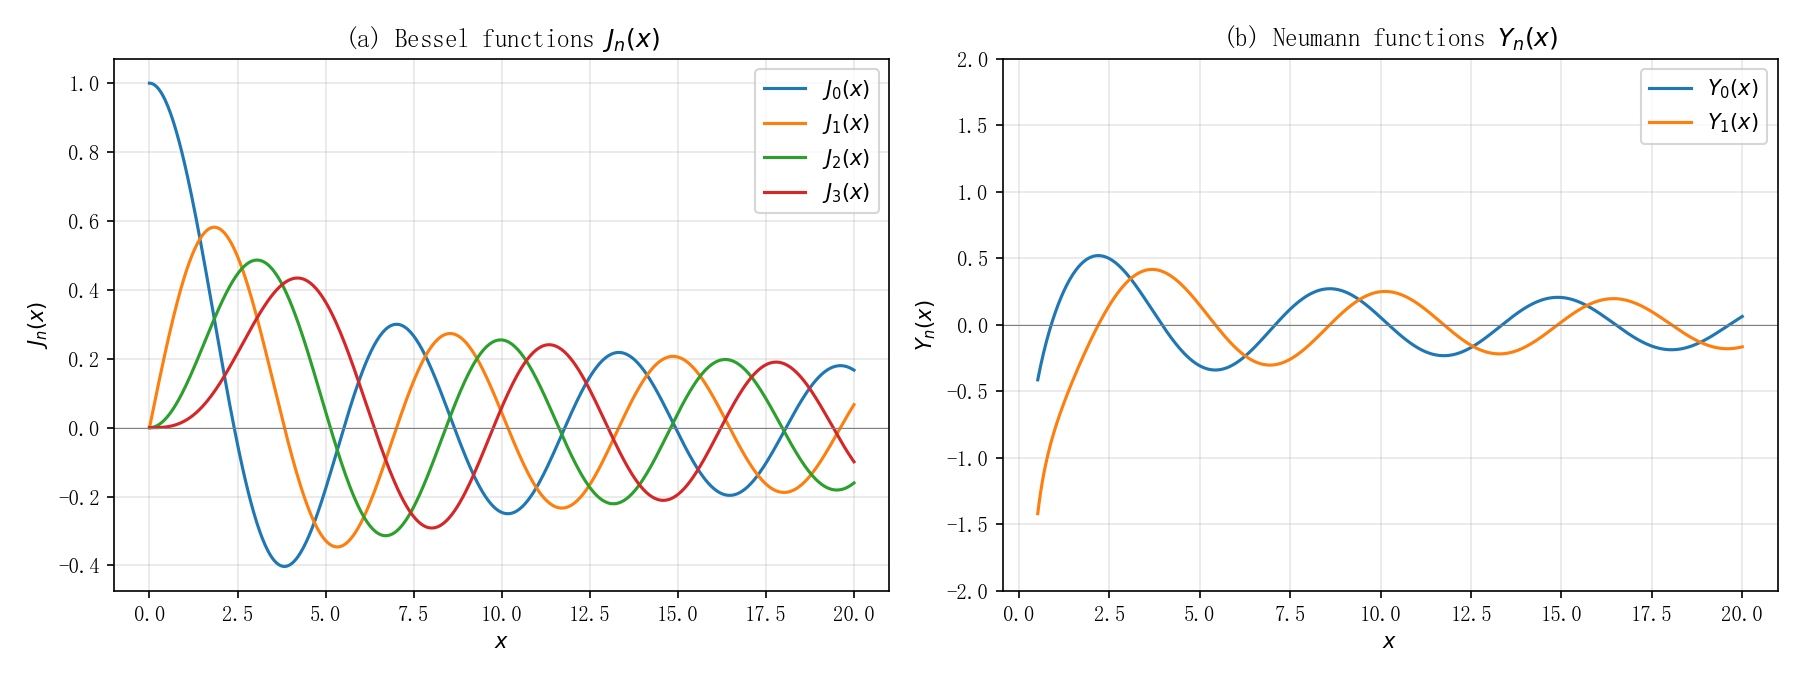
\includegraphics[width=0.85\textwidth]{figures/fig4_3_bessel.png}
\caption{(a) 第一类贝塞尔函数 $J_n(x)$（$n=0,1,2,3$）。(b) 第二类（诺依曼函数）$Y_n(x)$。注意 $Y_n(0)\to -\infty$，因此在涉及原点的物理问题中通常只保留 $J_n$。}
\label{fig:bessel}
\end{figure}

\subsection{贝塞尔函数的正交性}

对于固定 $\nu$，设 $j_{\nu,n}$ 为 $J_\nu(x)=0$ 的第 $n$ 个正根。则 $\{J_\nu(j_{\nu,n}\,r/R)\}$ 在区间 $[0,R]$ 上关于权重 $r$ 正交：
\begin{equation}
\int_0^R J_\nu\!\left(\frac{j_{\nu,m}r}{R}\right)
J_\nu\!\left(\frac{j_{\nu,n}r}{R}\right) r\,\dd r
= \frac{R^2}{2}[J_{\nu+1}(j_{\nu,n})]^2\delta_{mn}.
\label{eq:bessel_ortho}
\end{equation}

\subsection{物理应用：圆膜振动——完整算例}

\begin{example}[圆形鼓膜的振动模式]
\textbf{问题：} 半径为 $a$ 的圆形鼓膜，边界固定 $u(a,\phi)=0$。求振动模式（本征频率和本征函数）。

\textbf{步骤 1：建立极坐标波动方程。}
\begin{equation}
\frac{\partial^2 u}{\partial t^2} = c^2\left[
\frac{1}{r}\frac{\partial}{\partial r}\left(r\frac{\partial u}{\partial r}\right)
+ \frac{1}{r^2}\frac{\partial^2 u}{\partial\phi^2}
\right].
\end{equation}

\textbf{步骤 2：分离变量。}
$u(r,\phi,t)=R(r)\Phi(\phi)T(t)$。
\begin{align}
\frac{T''}{c^2 T} &= -k^2,\\
\frac{\Phi''}{\Phi} &= -m^2,\\
r^2 R'' + rR' + (k^2 r^2 - m^2)R &= 0.
\end{align}

\textbf{步骤 3：时间解。}
$T'' + k^2 c^2 T = 0 \Rightarrow T(t) = A\cos(\omega t) + B\sin(\omega t)$，其中 $\omega = kc$。

\textbf{步骤 4：角向解。}
$\Phi(\phi) = e^{\mathrm{i}m\phi}$，$m=0,1,2,\dots$（周期性要求 $m$ 为整数）。

\textbf{步骤 5：径向解——贝塞尔函数。}
径向方程是 $\nu=m$ 的贝塞尔方程。解为 $R(r) = J_m(kr)$（要求 $r=0$ 处有限，排除 $Y_m$）。

\textbf{步骤 6：边界条件确定 $k$。}
$u(a,\phi,t)=0 \Rightarrow R(a)=0 \Rightarrow J_m(ka)=0$。
令 $j_{m,n}$ 为 $J_m$ 的第 $n$ 个正零点，则 $k = j_{m,n}/a$，$n=1,2,3,\dots$。

\textbf{步骤 7：本征频率。}
\begin{equation}
\boxed{\;\omega_{mn} = c\,\frac{j_{m,n}}{a},\qquad
f_{mn} = \frac{c\,j_{m,n}}{2\pi a}\;}.
\end{equation}

\textbf{步骤 8：物理解读。}
基频：$(m,n)=(0,1)$ 对应 $j_{0,1}\approx 2.405$，$f_{01}=0.383c/a$——全膜同向振动。
一阶泛音：$(m,n)=(1,1)$ 对应 $j_{1,1}\approx 3.832$，有一条直径节线。
这些频率并非整数倍关系——鼓的声音"不和谐"的数学根源正在于此。
\end{example}

% 圆膜振动模式
\begin{figure}[H]
\centering
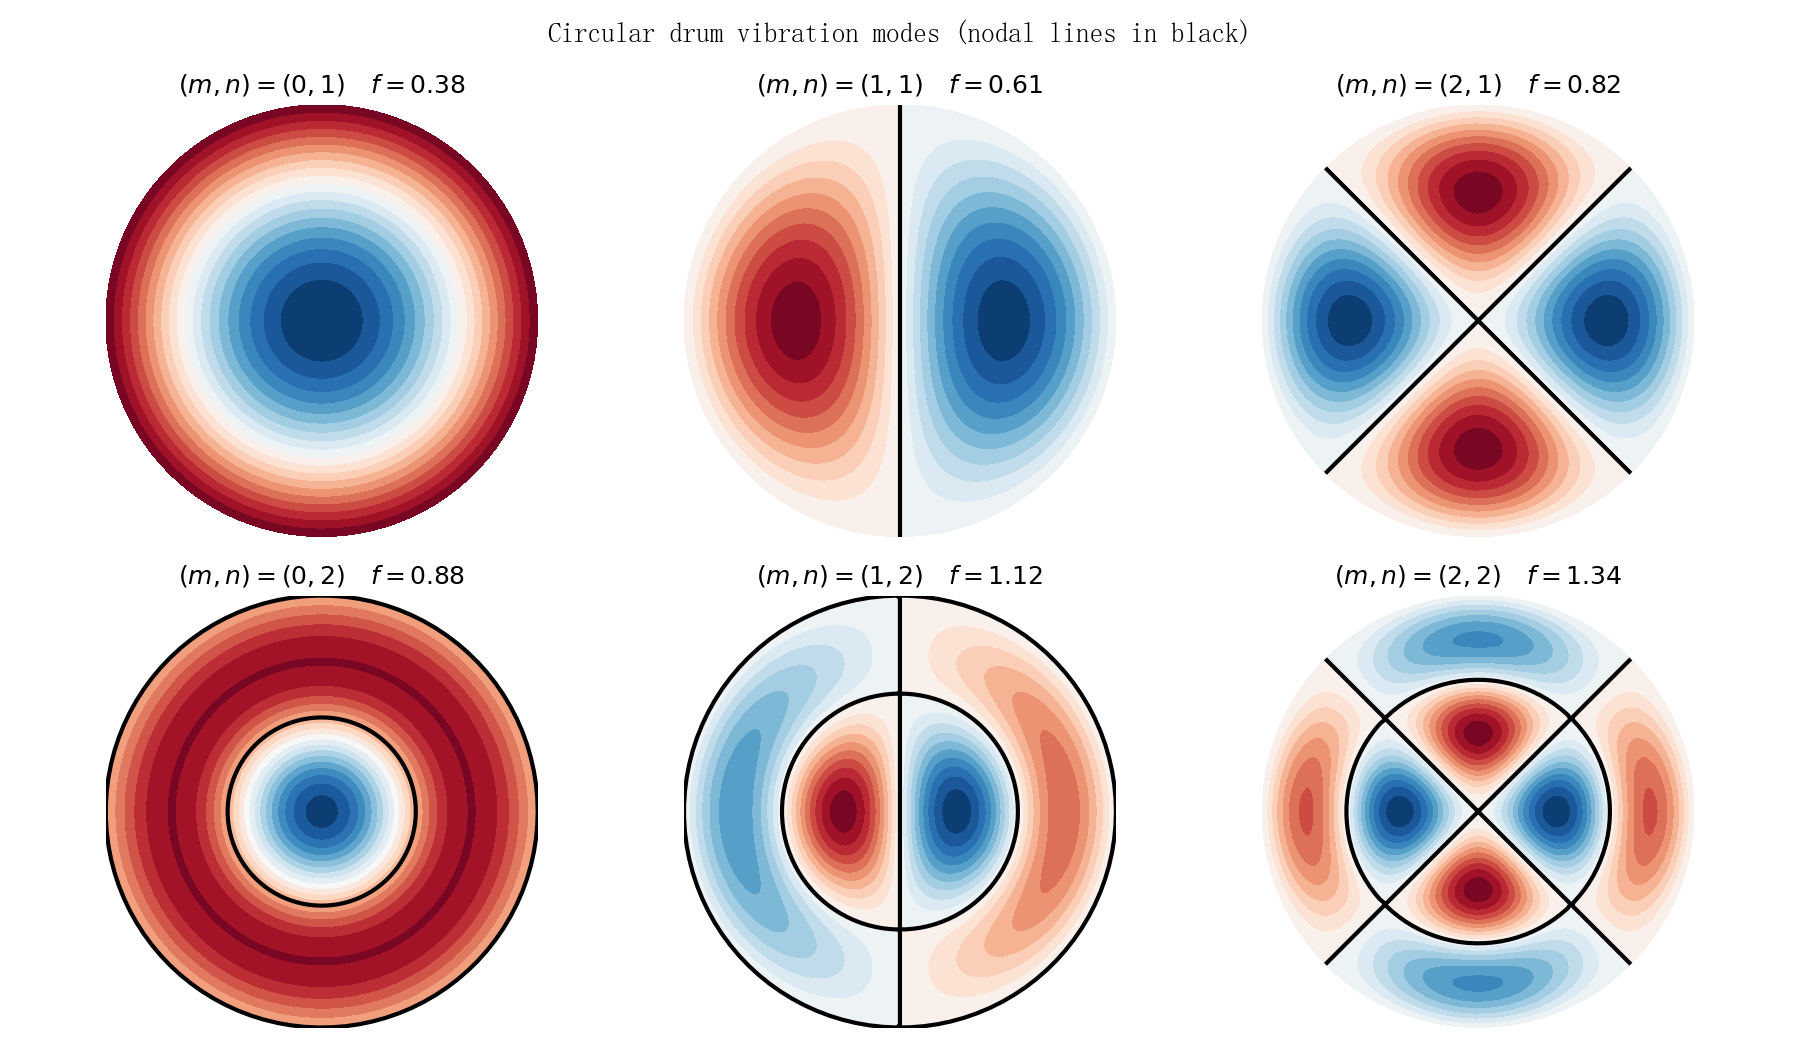
\includegraphics[width=0.85\textwidth]{figures/fig4_4_drum_modes.png}
\caption{圆膜的振动模式。颜色表位移，黑线为节线（位移恒为零的线）。$(m,n)$ 中 $m$ 为直径节线数，$n$ 为环向节线数。频率 $f$ 增加随 $m,n$ 增大而增大。}
\label{fig:drum_modes}
\end{figure}

\section{埃尔米特多项式与量子谐振子}
\label{sec:hermite}

\subsection*{动机：为什么量子谐振子产生离散能级？}

量子谐振子 $V(x) = \frac12 m\omega^2 x^2$ 的定态薛定谔方程在分离变量后，自然引出埃尔米特方程。其解——埃尔米特多项式——的正交性和递推关系直接给出了能级的量子化结构和升降算符。

\subsection{量子谐振子的定态薛定谔方程}

一维谐振子的定态薛定谔方程：
\begin{equation}
-\frac{\hbar^2}{2m}\frac{\dd^2\psi}{\dd x^2} + \frac12 m\omega^2 x^2\psi = E\psi.
\end{equation}

引入无量纲变量 $\xi = \sqrt{m\omega/\hbar}\,x$，方程化为：
\begin{equation}
\frac{\dd^2\psi}{\dd\xi^2} + (\epsilon - \xi^2)\psi = 0,\quad \epsilon = \frac{2E}{\hbar\omega}.
\label{eq:hermite_ode_raw}
\end{equation}

\subsection{埃尔米特方程与多项式}

设 $\psi(\xi) = H(\xi)e^{-\xi^2/2}$，代入后得到\textbf{埃尔米特方程}：
\begin{equation}
\frac{\dd^2 H}{\dd\xi^2} - 2\xi\frac{\dd H}{\dd\xi} + (\epsilon - 1)H = 0.
\label{eq:hermite_ode}
\end{equation}

要求波函数在无穷远处有限，迫使 $\epsilon - 1 = 2n$，即 $n=0,1,2,\dots$。此时方程的多项式解为\textbf{埃尔米特多项式}：

\begin{align}
H_0(\xi) &= 1,\\
H_1(\xi) &= 2\xi,\\
H_2(\xi) &= 4\xi^2 - 2,\\
H_3(\xi) &= 8\xi^3 - 12\xi,\\
H_4(\xi) &= 16\xi^4 - 48\xi^2 + 12.
\end{align}

\textbf{罗德里格斯公式：}
\begin{equation}
H_n(\xi) = (-1)^n e^{\xi^2}\frac{\dd^n}{\dd\xi^n}e^{-\xi^2}.
\label{eq:hermite_rodrigues}
\end{equation}

\textbf{正交性：}
\begin{equation}
\int_{-\infty}^{\infty} H_n(\xi)H_m(\xi)e^{-\xi^2}\,\dd\xi
= 2^n n!\sqrt{\pi}\,\delta_{nm}.
\label{eq:hermite_ortho}
\end{equation}

\textbf{递推关系：}
\begin{equation}
H_{n+1}(\xi) = 2\xi H_n(\xi) - 2n H_{n-1}(\xi),\qquad
H'_n(\xi) = 2n H_{n-1}(\xi).
\end{equation}

\subsection{量子谐振子的本征解}

\textbf{能级：}
\begin{equation}
E_n = \left(n + \frac12\right)\hbar\omega,\qquad n=0,1,2,\dots
\end{equation}

\textbf{本征函数：}
\begin{equation}
\psi_n(x) = \frac{1}{\sqrt{2^n n!}}\left(\frac{m\omega}{\pi\hbar}\right)^{1/4}
H_n\!\left(\sqrt{\frac{m\omega}{\hbar}}\,x\right) e^{-m\omega x^2/(2\hbar)}.
\label{eq:harmonic_oscillator_wf}
\end{equation}

\begin{insight}
埃尔米特多项式的递推关系 $H_{n+1} = 2\xi H_n - 2n H_{n-1}$ 在量子力学中有深刻的物理对应——它正是\textbf{升降算符} $\hat{a}^\dagger$ 和 $\hat{a}$ 作用的数学表现。这种代数方法（ ladder operator）远比直接求解微分方程优雅，也是量子场论中产生/湮灭算符的原型。
\end{insight}

\section{施图姆-刘维尔理论}
\label{sec:sturm_liouville}

\subsection*{动机：为什么所有特殊函数都有相同的正交性？}

勒让德多项式的正交关系 $\int_{-1}^1 P_l P_{l'} = 2/(2l+1)\delta_{ll'}$ 和贝塞尔函数的正交关系 $\int_0^R J_m(jr/R)J_m(j'r/R) r\,dr \propto \delta_{jj'}$，虽然看起来不同，但本质上来自同一个原因：它们都是\textbf{自伴算符}的本征函数。这就是施图姆-刘维尔理论的意义——它统一了所有正交函数系。

\subsection{SL 问题的标准形式}

\begin{equation}
-\frac{\dd}{\dd x}\left[p(x)\frac{\dd y}{\dd x}\right] + q(x)y
= \lambda w(x)y,\qquad a<x<b,
\label{eq:sl_form}
\end{equation}
附加适当的边界条件。

\textbf{SL 理论的核心结论：}
\begin{enumerate}
\item 本征值 $\lambda_n$ 是实数，且构成递增序列 $\lambda_1<\lambda_2<\cdots\to\infty$。
\item 本征函数 $y_n(x)$ 关于权函数 $w(x)$ 正交：
\begin{equation}
\int_a^b y_n(x) y_m(x) w(x)\,\dd x = 0,\quad n\neq m.
\end{equation}
\item 本征函数构成完备集——任意满足边界条件的函数可按 $\{y_n\}$ 展开。
\end{enumerate}

\subsection{SL 问题的物理统一性}

\begin{table}[h]
\centering
\caption{施图姆-刘维尔问题物理实例}
\label{tab:sl_examples}
\begin{tabular}{c|c|c|c|c}
\toprule
方程 & $p(x)$ & $q(x)$ & $w(x)$ & 区间 \\
\midrule
简谐振荡 $X''+\lambda X=0$ & $1$ & $0$ & $1$ & $[0,L]$ \\
勒让德 & $1-x^2$ & $0$ & $1$ & $[-1,1]$ \\
贝塞尔 & $x$ & $\nu^2/x$ & $x$ & $[0,R]$ \\
埃尔米特 & $e^{-x^2}$ & $0$ & $e^{-x^2}$ & $(-\infty,\infty)$ \\
拉盖尔 & $xe^{-x}$ & $0$ & $e^{-x}$ & $[0,\infty)$ \\
\bottomrule
\end{tabular}
\end{table}

\begin{example}[将勒让德方程化为 SL 形式]
勒让德方程 $(1-x^2)y'' - 2xy' + l(l+1)y = 0$。

乘以 $1$，注意到 $-[(1-x^2)y']' = -(1-x^2)y'' + 2xy'$，而原方程中的 $-2xy'$ 来自这里。整理：
\begin{equation}
-\frac{\dd}{\dd x}\left[(1-x^2)\frac{\dd y}{\dd x}\right] = l(l+1)y.
\end{equation}
所以 $p(x)=1-x^2$, $q(x)=0$, $w(x)=1$, $\lambda = l(l+1)$。区间 $[-1,1]$，边界条件为 $y(\pm1)$ 有界。
\end{example}

\begin{example}[将贝塞尔方程化为 SL 形式]
贝塞尔方程 $x^2 y'' + xy' + (x^2 - \nu^2)y = 0$ 除以 $x$：
\begin{equation}
xy'' + y' + \left(x - \frac{\nu^2}{x}\right)y = 0.
\end{equation}
写成 SL 形式：
\begin{equation}
-\frac{\dd}{\dd x}\left(x\frac{\dd y}{\dd x}\right) + \frac{\nu^2}{x}y = \lambda x y.
\end{equation}
所以 $p(x)=x$, $q(x)=\nu^2/x$, $w(x)=x$, $\lambda = k^2$（其中 $k$ 来自分离常数）。
\end{example}

\begin{insight}
施图姆-刘维尔理论是\textbf{量子力学中厄米算符谱定理}的经典原型。SL 算符 $\hat{L} = -\frac{\dd}{\dd x}p\frac{\dd}{\dd x}+q$ 在合适的函数空间中是自伴的（相当于厄米的），这正是为什么它的本征函数是正交完备的。量子力学中 $\hat{H}$ 的本征函数正交完备性，是 SL 理论在无限维空间的直接推广。
\end{insight}

\section{球贝塞尔函数}
\label{sec:spherical_bessel}

在三维波动方程和薛定谔方程的径向部分（球坐标），还会遇到\textbf{球贝塞尔方程}：
\begin{equation}
r^2\frac{\dd^2 R}{\dd r^2} + 2r\frac{\dd R}{\dd r}
+ [k^2 r^2 - l(l+1)]R = 0.
\label{eq:spherical_bessel_ode}
\end{equation}

其解为\textbf{球贝塞尔函数}：
\begin{equation}
j_l(x) = \sqrt{\frac{\pi}{2x}}J_{l+1/2}(x),\qquad
n_l(x) = \sqrt{\frac{\pi}{2x}}Y_{l+1/2}(x).
\label{eq:spherical_bessel}
\end{equation}
其中 $j_l$ 在 $x=0$ 处有限，$n_l$ 在 $x=0$ 处发散。

\textbf{前几个球贝塞尔函数：}
\begin{align}
j_0(x) &= \frac{\sin x}{x},\\
j_1(x) &= \frac{\sin x}{x^2} - \frac{\cos x}{x},\\
j_2(x) &= \left(\frac{3}{x^3} - \frac{1}{x}\right)\sin x - \frac{3}{x^2}\cos x.
\end{align}

\textbf{物理应用：}
\begin{itemize}
\item \textbf{量子散射：} 平面波可按球面波展开（Rayleigh 展开）：
\begin{equation}
e^{\mathrm{i}kz} = \sum_{l=0}^{\infty} (2l+1)\mathrm{i}^l j_l(kr) P_l(\cos\theta).
\end{equation}
\item \textbf{氢原子：} 径向波函数 $R_{nl}(r) \propto r^l e^{-r/(na_0)} L_{n-l-1}^{2l+1}(2r/(na_0))$，但在动量空间表述中会出现球贝塞尔函数。
\item \textbf{电磁散射（Mie 理论）：} 球体的电磁散射解用球贝塞尔和球汉克尔函数表达。
\end{itemize}

\section{本章小结}

\begin{itemize}
\item \textbf{三大经典 PDE——波动（双曲型）、热传导（抛物型）、泊松（椭圆型）}——覆盖了物理中所有重要的连续介质理论。
\item \textbf{分离变量法} 将 PDE 化为 ODE，在其中自然出现特殊函数。
\item \textbf{勒让德多项式} 源于球对称问题的角向方程，用于多极展开和球面上的函数展开。
\item \textbf{贝塞尔函数} 源于柱/球对称问题的径向方程，描述带有几何扩散的波动和扩散过程。
\item \textbf{埃尔米特多项式} 源于量子谐振子问题，是升降算符方法的数学基础。
\item \textbf{施图姆-刘维尔理论} 统一了所有正交函数系，为量子力学的谱理论提供了数学典范。
\end{itemize}

\subsection*{概念图谱}

\begin{center}
\fbox{\parbox{0.92\textwidth}{
\textbf{PDE 与特殊函数的概念网络：}\\[3pt]
$\bullet$ 波动方程（双曲）$\leftrightarrow$ 热传导方程（抛物）$\leftrightarrow$ 拉普拉斯方程（椭圆）\\[3pt]
$\bullet$ 分离变量 $\to$ 本征值问题 $\to$ 特殊函数正交系\\[3pt]
$\bullet$ 球对称 $\to$ 勒让德多项式 $P_l(x)$ / 球谐函数 $Y_{lm}$ / 球贝塞尔函数 $j_l(x)$\\[3pt]
$\bullet$ 柱对称 $\to$ 贝塞尔函数 $J_m(x)$\\[3pt]
$\bullet$ 谐振子 $\to$ 埃尔米特多项式 $H_n(\xi)$\\[3pt]
$\bullet$ SL 理论：$-(py')' + qy = \lambda w y$ $\to$ 统一框架
}}
\end{center}

\subsection*{公式参考表}

\begin{table}[h]
\centering
\caption{特殊函数核心公式速查}
\label{tab:special_func_formulas}
\begin{tabular}{c|c}
\toprule
公式 & 说明 \\
\midrule
$P_l(x) = \frac{1}{2^l l!}\frac{d^l}{dx^l}(x^2-1)^l$ & 勒让德多项式（Rodrigues） \\
$\int_{-1}^1 P_l(x)P_{l'}(x)\,dx = \frac{2}{2l+1}\delta_{ll'}$ & 勒让德正交性 \\
$J_\nu(x) = \sum_{k=0}^\infty \frac{(-1)^k}{k!\Gamma(\nu+k+1)}(x/2)^{\nu+2k}$ & 贝塞尔函数级数 \\
$J_\nu(x) \sim \sqrt{\frac{2}{\pi x}}\cos(x - \frac{\nu\pi}{2} - \frac{\pi}{4})$ & 贝塞尔渐近形式 \\
$\int_0^R J_\nu(j_{\nu,m}r/R)J_\nu(j_{\nu,n}r/R)\,r\,dr \propto \delta_{mn}$ & 贝塞尔正交性 \\
$H_n(\xi) = (-1)^n e^{\xi^2}\frac{d^n}{d\xi^n}e^{-\xi^2}$ & 埃尔米特多项式 \\
$\int_{-\infty}^\infty H_n(\xi)H_m(\xi)e^{-\xi^2}\,d\xi = 2^n n!\sqrt{\pi}\delta_{nm}$ & 埃尔米特正交性 \\
$E_n = (n+1/2)\hbar\omega$ & 谐振子能级 \\
$Y_{lm}(\theta,\phi) \propto P_l^m(\cos\theta)e^{im\phi}$ & 球谐函数 \\
$-(py')' + qy = \lambda w y$ & SL 标准形式 \\
\bottomrule
\end{tabular}
\end{table}

\begin{insight}[第 4 章的核心思维链条]
\textbf{物理问题 $\to$ 三大 PDE 分类 $\to$ 对称性引导坐标系选择 $\to$ 分离变量 $\to$ 本征值问题 $\to$ 特殊函数自然涌现 $\to$ SL 理论统一框架。} 特殊函数不是数学家臆造的，而是物理对称性（球对称 $\to$ 勒让德，柱对称 $\to$ 贝塞尔）在求解 PDE 过程中不可回避的产物。
\end{insight}

\section*{习题}

\textbf{基础题（巩固概念）}

\begin{enumerate}
\item 判断下列方程的类型并写出特征线（如果有）：
(1) $u_{tt} - c^2 u_{xx} = 0$；(2) $u_t = \kappa u_{xx}$；
(3) $u_{xx} + u_{yy} = 0$；(4) $u_{xx} + 2u_{xy} + u_{yy} = 0$。
\item 用分离变量法求解矩形膜 $(0<x<a,\;0<y<b)$ 的波动方程，边界固定，初始位移为零，初始速度为 $g(x,y)$。写出本征频率。
\item 证明勒让德多项式的正交关系 $\int_{-1}^1 P_l(x)P_{l'}(x)\,\dd x = \frac{2}{2l+1}\delta_{ll'}$。
\item 写出半径为 $R$ 的无限长圆柱体内部拉普拉斯方程的通解，设边界条件为 $u(R,\phi)=V_0\cos\phi$。\textbf{提示：} 解应为 $u(r,\phi)=Ar\cos\phi$。
\item 写出前三个埃尔米特多项式 $H_0,H_1,H_2$，并验证它们满足埃尔米特方程。
\item 验证 $j_0(x)$ 和 $j_1(x)$ 满足球贝塞尔方程。
\end{enumerate}

\textbf{提高题（应用分析）}

\begin{enumerate}
\item[7.] 半径为 $R$ 的无限长圆柱体，侧面电势为 $V_0$（与 $\phi$ 无关），求内部电势分布。将解写为贝塞尔函数的级数形式。
\item[8.] 一圆形鼓膜半径为 $a$，初始位移为 $f(r) = h(1 - r^2/a^2)$，初始速度为零。求其振动规律。摩擦使振动衰减，定性地说明加入阻尼项 $\gamma u_t$ 后的效果。
\item[9.] 球贝塞尔函数 $j_l(x)$ 满足递推关系 $j_{l+1}(x) = \frac{2l+1}{x}j_l(x) - j_{l-1}(x)$。验证 $l=0$ 和 $l=1$ 的情形。
\item[10.] 将函数 $f(x)=\Theta(1-|x|)$ 在勒让德多项式基下展开到 $l=4$ 项。
\item[11.] 求量子谐振子的基态 $\psi_0(x)$ 和第一激发态 $\psi_1(x)$ 的显式表达式。验证 $\psi_0$ 和 $\psi_1$ 正交。
\item[12.] 写出叠加原理：利用热传导方程的线性性质，由两个特解构造满足 $u(x,0)=3\sin(\pi x/L)-2\sin(2\pi x/L)$ 的解。
\end{enumerate}

\textbf{挑战题（综合拓展）}

\begin{enumerate}
\item[13.]（氢原子的径向方程）写出氢原子 $V(r)=-e^2/(4\pi\varepsilon_0 r)$ 的薛定谔方程。分离变量后，证明径向方程可以通过变量替换化为缔合拉盖尔方程，并说明 $n$（主量子数）的出现。
\item[14.]（球谐函数的加法公式）证明 $\sum_{m=-l}^l Y_{lm}^*(\theta',\phi')Y_{lm}(\theta,\phi) = \frac{2l+1}{4\pi}P_l(\cos\gamma)$，其中 $\gamma$ 是 $(\theta,\phi)$ 和 $(\theta',\phi')$ 之间的夹角。这个公式在量子散射和 CMB 分析中至关重要。
\item[15.]（用格林函数求解泊松方程）写出点源泊松方程 $\nabla^2 G(\mathbf{r},\mathbf{r}') = \delta(\mathbf{r}-\mathbf{r}')$ 在无界空间中的解 $G(\mathbf{r},\mathbf{r}') = -1/(4\pi|\mathbf{r}-\mathbf{r}'|)$。利用格林恒等式说明它为何可以构造任意分布 $\rho(\mathbf{r})$ 的解。
\item[16.]（数值计算）编写 Python 代码，计算圆形膜 $(m,n)=(0,1)$ 和 $(1,1)$ 的本征频率和本征函数。用 matplotlib 绘制前 4 个模式的位移分布图。
\item[17.]（相干态）证明量子谐振子的相干态 $\psi_\alpha(x)$ 是最小不确定波包，且满足 $\Delta x \Delta p = \hbar/2$。利用埃尔米特多项式的生成函数写出相干态的显式表达式。
\item[18.]（非均匀弦的振动）一根密度不均匀的弦 $\rho(x) = \rho_0(1 + \varepsilon x/L)$，写出其振动方程并化为 SL 形式。讨论本征频率如何随 $\varepsilon$ 变化。
\end{enumerate}

% ============================================================
%  第 5 章  数值方法：有限差分与 SciPy 计算（扩展版）
% ============================================================

\chapter{数值方法：有限差分与 SciPy 计算}

\section{本章概览与学习路线}

前三章建立了物理问题的解析框架：分离变量、特殊函数、积分变换。但现实世界远比教科书复杂——非均匀介质、非线性项、不规则边界，这些都会使解析解遥不可及。

数值方法不是解析方法的替代，而是\textbf{互补}：
\begin{itemize}
\item 解析解提供物理洞察和参数标度律。
\item 数值解提供特定条件下的定量预言。
\end{itemize}

本章以\textbf{有限差分法} 为主线，结合 Python 的 NumPy/SciPy 生态，让你亲手"计算"前三章的偏微分方程。你将看到分离变量法给出的本征函数如何转化为矩阵本征值问题，傅里叶变换如何用 FFT 在 $O(N\log N)$ 时间内完成。

\begin{center}
\fbox{\parbox{0.9\textwidth}{\centering
\textbf{核心逻辑链条：}\\
连续 PDE $\to$ 网格离散 $\to$ 差分近似 $\to$ 稀疏矩阵 $\to$ 代数方程组求解
}}
\end{center}

\subsection*{不同读者的学习路径}

\begin{itemize}
\item \textbf{物理专业学生：} 重点关注 \S5.2--\S5.5（有限差分基础与 PDE 离散化），\S5.7（矩阵本征值问题——量子力学的数值视角），\S5.8（FFT 与谱方法）。
\item \textbf{计算科学学生：} 重点关注 \S5.2（截断误差与收敛性分析），\S5.3--\S5.5（不同时间步进格式的稳定性），\S5.10（误差分析与网格收敛性研究）。
\item \textbf{工程学生：} 重点关注 \S5.3--\S5.6（综合案例）中的可运行代码，直接应用于实际问题。
\end{itemize}

\section{有限差分基础}
\label{sec:fd_basics}

\subsection*{动机：计算机只能做加减乘除，如何让它求导？}

计算机不能理解 $\lim_{h\to 0}$，它只能计算加法、减法和乘法。有限差分的核心是放弃了"极限"，用一个小量 $h$ 来近似——这等价于把连续空间离散化为网格。放弃一定的精度换取可计算性，这就是数值分析的基本哲学。

\subsection{导数的差分近似}

由泰勒展开：
\begin{equation}
f(x+h) = f(x) + h f'(x) + \frac{h^2}{2}f''(x)
+ \frac{h^3}{6}f'''(x) + \cdots
\end{equation}

\textbf{一阶向前差分：}
\begin{equation}
f'(x) \approx \frac{f(x+h) - f(x)}{h},\quad \text{截断误差 } O(h).
\label{eq:forward_diff}
\end{equation}

\textbf{一阶向后差分：}
\begin{equation}
f'(x) \approx \frac{f(x) - f(x-h)}{h},\quad O(h).
\label{eq:backward_diff}
\end{equation}

\textbf{一阶中心差分：}
\begin{equation}
f'(x) \approx \frac{f(x+h) - f(x-h)}{2h},\quad O(h^2).
\label{eq:central_diff}
\end{equation}

\textbf{二阶中心差分：}
\begin{equation}
f''(x) \approx \frac{f(x+h) - 2f(x) + f(x-h)}{h^2},\quad O(h^2).
\label{eq:second_diff}
\end{equation}

\subsection{截断误差的详细推导}

以二阶中心差分为例，写出 $f(x\pm h)$ 的泰勒展开：
\begin{align}
f(x+h) &= f(x) + hf'(x) + \frac{h^2}{2}f''(x) + \frac{h^3}{6}f'''(x) + \frac{h^4}{24}f^{(4)}(x) + \cdots,\\
f(x-h) &= f(x) - hf'(x) + \frac{h^2}{2}f''(x) - \frac{h^3}{6}f'''(x) + \frac{h^4}{24}f^{(4)}(x) + \cdots.
\end{align}

两式相加，消去奇数阶导数项：
\begin{equation}
f(x+h) + f(x-h) = 2f(x) + h^2 f''(x) + \frac{h^4}{12}f^{(4)}(x) + O(h^6).
\end{equation}

整理得：
\begin{equation}
f''(x) = \frac{f(x+h) - 2f(x) + f(x-h)}{h^2} - \frac{h^2}{12}f^{(4)}(x) + O(h^4).
\end{equation}

因此截断误差的主项是 $-\frac{h^2}{12}f^{(4)}(x)$，阶数为 $O(h^2)$。

\begin{insight}
中心差分比单侧差分精度高一个阶次，因为对称性消去了 $O(h)$ 项。这如同量子力学中中心势 $V(-x)=V(x)$ 使波函数具有确定宇称——对称性在这里简化了问题并提高了精度。
\end{insight}

% 有限差分模板图
\begin{figure}[H]
\centering
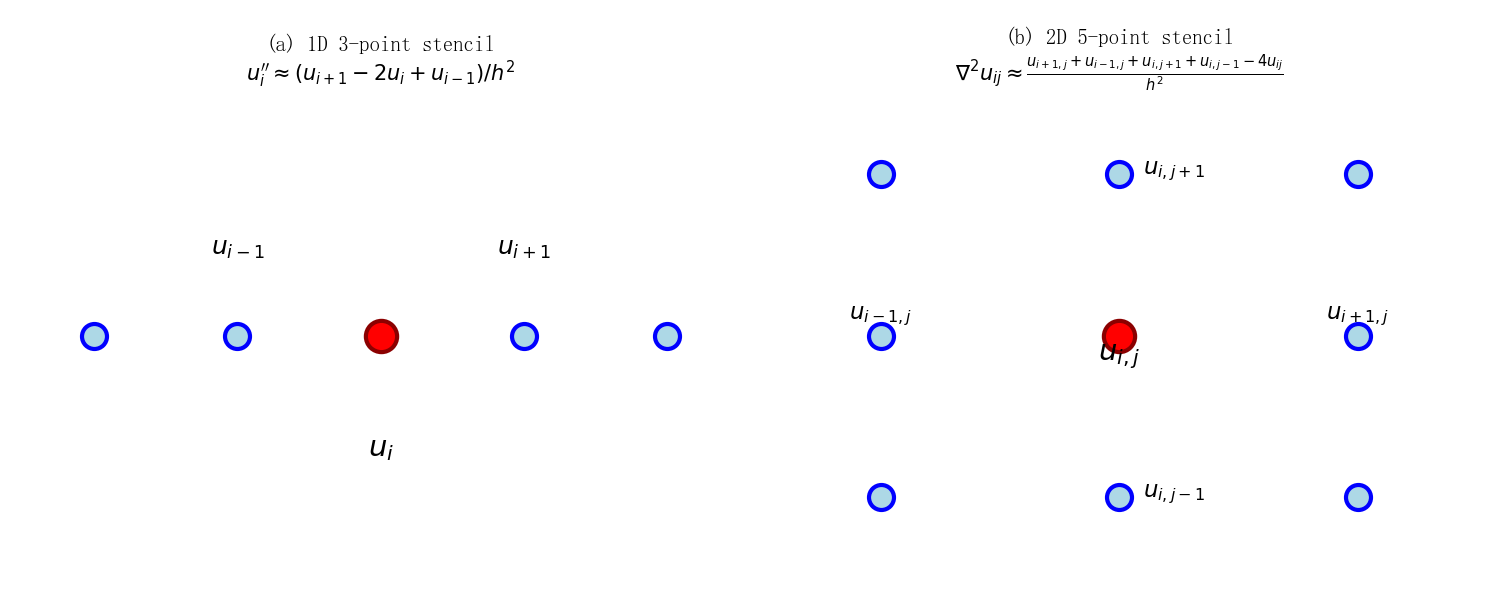
\includegraphics[width=0.8\textwidth]{figures/fig5_1_fd_stencil.png}
\caption{有限差分模板。左：一维三点模板，用于离散二阶导数。右：二维五点模板，用于离散拉普拉斯算子。红点为中心点 $u_{i,j}$，蓝点为邻点。}
\label{fig:fd_stencil}
\end{figure}

\subsection{差分模板与五点格式}

对于二维区域 $(x_i,y_j)$，拉普拉斯算子的五点差分格式为：
\begin{equation}
\nabla^2 u_{ij} \approx
\frac{u_{i+1,j} + u_{i-1,j} + u_{i,j+1} + u_{i,j-1} - 4u_{ij}}{h^2},
\label{eq:five_point}
\end{equation}
其中 $h = \Delta x = \Delta y$。截断误差 $O(h^2)$。

\subsection{收敛性初步}

有限差分法的误差来源于两个方面：
\begin{itemize}
\item \textbf{截断误差 (truncation error)}：由泰勒展开截断引起，当 $h\to0$ 时趋于零。
\item \textbf{舍入误差 (round-off error)}：由浮点数有限精度引起，当 $h$ 极小时占主导。
\end{itemize}

\textbf{收敛性：} 当 $h\to0$ 时，数值解趋近于精确解，称为方法收敛。对于相容且稳定的格式，Lax 等价定理保证收敛性。

\section{一维边值问题：泊松方程}
\label{sec:poisson1d}

\subsection{问题离散化}

考虑一维泊松方程：
\begin{equation}
-\frac{\dd^2 u}{\dd x^2} = f(x),\quad x\in(0,1),\quad u(0)=u(1)=0.
\label{eq:poisson1d}
\end{equation}

将区间 $[0,1]$ 分为 $N$ 等份，$x_i = i h$，$h=1/N$，$i=0,1,\dots,N$。

在内部点 $i=1,\dots,N-1$ 应用二阶中心差分：
\begin{equation}
-\frac{u_{i+1} - 2u_i + u_{i-1}}{h^2} = f_i.
\label{eq:poisson_discrete}
\end{equation}

写成矩阵形式 $A\mathbf{u} = \mathbf{f}$：
\begin{equation}
\frac{1}{h^2}\begin{pmatrix}
2 & -1 & 0 & \cdots & 0 \\
-1 & 2 & -1 & \cdots & 0 \\
0 & -1 & 2 & \cdots & 0 \\
\vdots & \vdots & \vdots & \ddots & \vdots \\
0 & 0 & 0 & \cdots & 2
\end{pmatrix}
\begin{pmatrix} u_1 \\ u_2 \\ u_3 \\ \vdots \\ u_{N-1} \end{pmatrix}
= \begin{pmatrix} f_1 \\ f_2 \\ f_3 \\ \vdots \\ f_{N-1} \end{pmatrix}.
\label{eq:poisson_matrix}
\end{equation}

这是一个\textbf{三对角矩阵}，可以用 $O(N)$ 的 Thomas 算法高效求解。

\subsection{Python 实现——完整可运行代码}

\begin{lstlisting}[language=Python, caption=一维泊松方程的有限差分求解]
import numpy as np
import matplotlib.pyplot as plt
from scipy import sparse
from scipy.sparse.linalg import spsolve

def poisson_1d(N=100):
    """求解 -u'' = f, u(0)=u(1)=0, f(x) = sin(pi*x)"""
    h = 1.0 / N
    x = np.linspace(0, 1, N+1)

    # 构造稀疏三对角矩阵
    e = np.ones(N-1)
    A = sparse.diags([-e, 2*e, -e], [-1, 0, 1],
                     shape=(N-1, N-1)) / h**2

    # 右端项 f(x) = sin(pi*x)
    f = np.sin(np.pi * x[1:-1])

    # 求解 Au = f
    u_interior = spsolve(A.tocsr(), f)

    # 添加边界条件
    u = np.zeros(N+1)
    u[1:-1] = u_interior

    # 解析解: u_exact = sin(pi*x) / pi^2
    u_exact = np.sin(np.pi * x) / np.pi**2

    return x, u, u_exact

x, u_num, u_ex = poisson_1d(N=50)
error = np.max(np.abs(u_num - u_ex))
print(f"Max error: {error:.2e}")
# N=50 时输出约 6.6e-4 (O(h^2) 收敛)
\end{lstlisting}

\subsection{稀疏矩阵为什么重要？}

如果使用 $N=1000$，满矩阵大小为 $999\times 999$，占用约 8 MB 内存。但 $N=10^5$ 时满矩阵需要 80 GB——不可接受！而三对角稀疏矩阵只需要 $O(N)$ 存储（约 2.4 MB 对 $N=10^5$）。

\begin{insight}
\textbf{稀疏矩阵是连接连续物理和离散计算的桥梁。} 有限差分产生的矩阵天然稀疏——每个内部点只与相邻点耦合。这对应于物理中的\textbf{局域性 (locality)}：一点的场只直接受其近邻影响。如果矩阵是稠密的，那意味着非局域相互作用，物理上通常对应更复杂的情况（如边界元法）。
\end{insight}

% 数值解对比图
\begin{figure}[H]
\centering
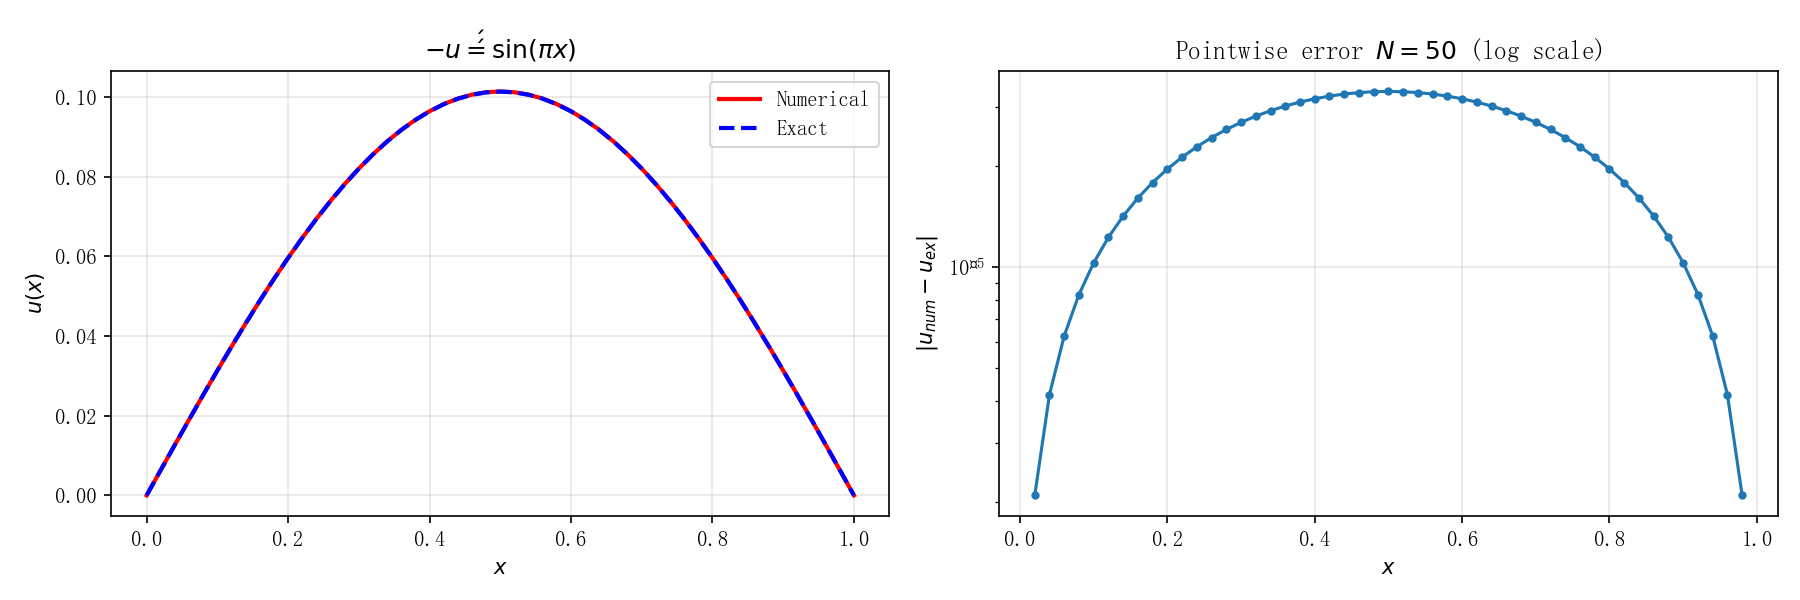
\includegraphics[width=0.85\textwidth]{figures/fig5_4_numerical_solution.png}
\caption{左：$-u''=\sin(\pi x)$ 的数值解与解析解对比（$N=50$），两者几乎完全重合。右：逐点误差（对数坐标），误差呈 $O(h^2)$ 量级。}
\label{fig:numerical_solution}
\end{figure}

\section{二维拉普拉斯方程}
\label{sec:laplace2d}

\subsection{五点差分与矩阵构造}

考虑 $[0,1]\times[0,1]$ 上的拉普拉斯方程 $\nabla^2 u = 0$，边界条件给定。

内部网格点 $(i,j)$，$i,j=1,\dots,M$，$h=1/(M+1)$：
\begin{equation}
u_{i+1,j} + u_{i-1,j} + u_{i,j+1} + u_{i,j-1} - 4u_{ij} = 0.
\label{eq:laplace2d_discrete}
\end{equation}

将所有 $M^2$ 个未知数排成列向量 $\mathbf{u}$（按行优先），则矩阵 $A$ 是 $M^2\times M^2$ 的\textbf{块三对角矩阵}：
\begin{equation}
A = \begin{pmatrix}
T & -I & 0 & \cdots & 0 \\
-I & T & -I & \cdots & 0 \\
0 & -I & T & \cdots & 0 \\
\vdots & \vdots & \vdots & \ddots & \vdots \\
0 & 0 & 0 & \cdots & T
\end{pmatrix},\qquad
T = \begin{pmatrix}
4 & -1 & 0 & \cdots \\
-1 & 4 & -1 & \cdots \\
\vdots & \vdots & \vdots & \ddots
\end{pmatrix}_{M\times M}.
\label{eq:block_tridiag}
\end{equation}

\begin{lstlisting}[language=Python, caption=二维拉普拉斯方程的有限差分]
import numpy as np
from scipy import sparse
from scipy.sparse.linalg import spsolve

def laplace_2d(M=50):
    """五点差分求解二维拉普拉斯方程"""
    h = 1.0 / (M + 1)
    N = M * M  # 未知数总数

    # 构造块三对角矩阵
    e = np.ones(M)
    T = sparse.diags([-e, 4*e, -e], [-1, 0, 1], shape=(M, M))
    I = sparse.eye(M)

    A = (sparse.kron(sparse.eye(M), T)
         + sparse.kron(sparse.diags([e], [-1], shape=(M, M)), -I)
         + sparse.kron(sparse.diags([e], [1], shape=(M, M)), -I))

    # 边界条件: u=0 在上边界 (y=1), 其余边界 u=0
    f = np.zeros(N)
    x = np.linspace(0, 1, M+2)[1:-1]
    u_top = np.sin(np.pi * x)
    for j in range(M):
        idx = (M-1)*M + j  # 最后一行
        f[idx] += u_top[j] / h**2

    u_flat = spsolve(A.tocsr(), f)
    u = u_flat.reshape((M, M))
    return u

u = laplace_2d(M=40)
print(f"Solution shape: {u.shape}")
# 输出: Solution shape: (40, 40)
\end{lstlisting}

% 稀疏矩阵结构图
\begin{figure}[H]
\centering
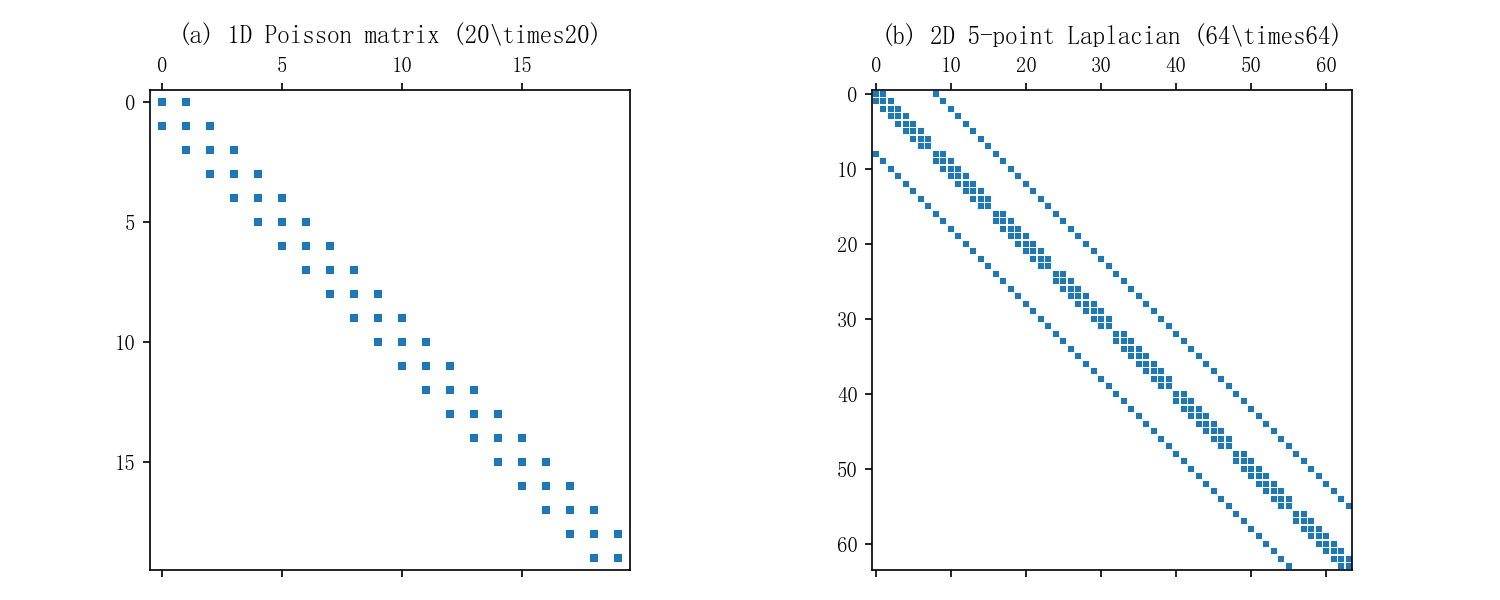
\includegraphics[width=0.8\textwidth]{figures/fig5_2_sparse_pattern.png}
\caption{稀疏矩阵非零模式（Spy 图）。左：一维泊松矩阵是标准三对角结构。右：二维五点拉普拉斯矩阵是块三对角结构，非零元素仅占 $O(N)$。}
\label{fig:sparse_pattern}
\end{figure}

\section{热传导方程：时间依赖问题}
\label{sec:heat_fd}

\subsection{显式欧拉法}

一维热传导方程 $u_t = \kappa u_{xx}$：
\begin{equation}
u_i^{n+1} = u_i^n + \frac{\kappa\Delta t}{h^2}
\left(u_{i+1}^n - 2u_i^n + u_{i-1}^n\right).
\label{eq:explicit_euler}
\end{equation}

\textbf{稳定性条件 (CFL 条件)：}
\begin{equation}
r = \frac{\kappa\Delta t}{h^2} \leq \frac{1}{2}.
\label{eq:cfl_condition}
\end{equation}

如果 $r>1/2$，数值解会指数增长——这是因为显式格式的放大因子 $|1 - 4r\sin^2(kh/2)| > 1$ 对高频模成立。

\begin{insight}[CFL 条件的物理解读]
CFL 条件 $r \leq 1/2$ 的物理解读：在一个时间步内，信息最多只能传播一个网格间距。如果 $\Delta t$ 太大，数值格式就"看不到"相邻网格点之间的物理耦合，导致不稳定。这呼应了波动方程中双曲型 PDE 的有限传播速度——数值稳定性与物理因果性在这里达成了一致。
\end{insight}

\subsection{隐式欧拉法与 Crank-Nicolson 格式}

用 $n+1$ 时刻的空间差分代替 $n$ 时刻：
\begin{equation}
u_i^{n+1} - \frac{\kappa\Delta t}{h^2}
\left(u_{i+1}^{n+1} - 2u_i^{n+1} + u_{i-1}^{n+1}\right) = u_i^n.
\label{eq:implicit_euler}
\end{equation}

\textbf{无条件稳定！} 代价是每步需要求解一个三对角线性系统。

\textbf{Crank-Nicolson 方法}（结合显式和隐式，精度 $O(\Delta t^2 + h^2)$）：
\begin{equation}
u_i^{n+1} - \frac{r}{2}\left(u_{i+1}^{n+1} - 2u_i^{n+1} + u_{i-1}^{n+1}\right)
= u_i^n + \frac{r}{2}\left(u_{i+1}^n - 2u_i^n + u_{i-1}^n\right).
\label{eq:crank_nicolson}
\end{equation}

\begin{lstlisting}[language=Python, caption=Crank-Nicolson 法求解热传导方程]
import numpy as np
from scipy import sparse
from scipy.sparse.linalg import spsolve

def heat_cn(Nx=100, Nt=500, T_final=0.1):
    """Crank-Nicolson 求解 u_t = u_xx
       边界: u(0)=u(1)=0
       初始: u(x,0) = sin(pi*x) + 0.5*sin(3*pi*x)
    """
    h = 1.0 / Nx
    dt = T_final / Nt
    r = dt / h**2  # kappa=1

    x = np.linspace(0, 1, Nx+1)
    u = np.sin(np.pi*x) + 0.5*np.sin(3*np.pi*x)
    u[0] = u[-1] = 0

    # 隐式系统矩阵 (三对角)
    e = np.ones(Nx-1)
    A = sparse.diags([-r/2*e, (1+r)*e, -r/2*e],
                     [-1, 0, 1], shape=(Nx-1, Nx-1))
    B = sparse.diags([r/2*e, (1-r)*e, r/2*e],
                     [-1, 0, 1], shape=(Nx-1, Nx-1))

    for n in range(Nt):
        u[1:-1] = spsolve(A, B @ u[1:-1])

    # 解析解
    u_exact = (np.exp(-np.pi**2*T_final)*np.sin(np.pi*x)
               + 0.5*np.exp(-9*np.pi**2*T_final)*np.sin(3*np.pi*x))
    error = np.max(np.abs(u - u_exact))
    return x, u, error

x, u, err = heat_cn(Nx=100, Nt=500, T_final=0.1)
print(f"Crank-Nicolson error: {err:.2e}")
# Nx=100, Nt=500 时误差约 1e-5
\end{lstlisting}

\subsection{三种时间步进格式的对比}

\begin{table}[h]
\centering
\caption{热传导方程三种时间步进格式对比}
\label{tab:time_stepping}
\begin{tabular}{c|c|c|c}
\toprule
格式 & 稳定性 & 每步计算量 & 精度 \\
\midrule
显式 Euler & $r \leq 1/2$ & $O(N)$ & $O(\Delta t)$ \\
隐式 Euler & 无条件稳定 & 解三对角系统 & $O(\Delta t)$ \\
Crank-Nicolson & 无条件稳定 & 解三对角系统 & $O(\Delta t^2)$ \\
\bottomrule
\end{tabular}
\end{table}

\section{波动方程：时域有限差分}
\label{sec:wave_fd}

一维波动方程 $u_{tt} = c^2 u_{xx}$，用中心差分近似时间二阶导：
\begin{equation}
\frac{u_i^{n+1} - 2u_i^n + u_i^{n-1}}{\Delta t^2}
= c^2\frac{u_{i+1}^n - 2u_i^n + u_{i-1}^n}{h^2}.
\label{eq:wave_fd}
\end{equation}

\textbf{显式递推公式：}
\begin{equation}
u_i^{n+1} = 2u_i^n - u_i^{n-1}
+ \frac{c^2\Delta t^2}{h^2}\left(u_{i+1}^n - 2u_i^n + u_{i-1}^n\right).
\label{eq:wave_explicit}
\end{equation}

\textbf{CFL 稳定条件：} $\dfrac{c\Delta t}{h} \leq 1$。这正好是物理因果性的数值体现——数值域必须包含物理解依赖域。

\begin{lstlisting}[language=Python, caption=波动方程的时域有限差分]
import numpy as np

def wave_1d(Nx=200, c=1.0, T_final=2.0):
    """一维波动方程 FDTD 求解"""
    h = 2.0 / Nx  # x in [-1, 1]
    dt = 0.5 * h / c  # CFL = 0.5
    Nt = int(T_final / dt)

    x = np.linspace(-1, 1, Nx+1)
    r = (c * dt / h)**2

    # 初始高斯波包
    u0 = np.exp(-50 * x**2)
    u_prev = u0.copy()
    u_curr = u0.copy()
    u_next = np.zeros(Nx+1)

    # 第一步: 初始速度 = 0 => u_curr = u0 + 0.5*dt^2*u_tt
    u_curr[1:-1] = u0[1:-1] + 0.5 * r * (
        u0[2:] - 2*u0[1:-1] + u0[:-2])

    for n in range(1, Nt):
        u_next[1:-1] = (2*u_curr[1:-1] - u_prev[1:-1]
                        + r*(u_curr[2:] - 2*u_curr[1:-1] + u_curr[:-2]))
        u_prev, u_curr, u_next = u_curr, u_next, u_prev

    return x, u_curr
# 初始高斯波包在 t=2 时应分裂为两个半波包
# 分别运行至 x = ±c*t = ±2
\end{lstlisting}

\section{矩阵本征值问题与 SciPy}
\label{sec:eigenvalue}

\subsection{从量子力学到数值本征值}

一维薛定谔方程 $-\dfrac{\hbar^2}{2m}\psi'' + V(x)\psi = E\psi$ 离散化后变为矩阵本征值问题：
\begin{equation}
H\mathbf{\psi} = E\mathbf{\psi},
\end{equation}
其中 $H$ 是 $N\times N$ 的三对角矩阵。

\begin{lstlisting}[language=Python, caption=一维无限深势阱的数值本征值]
import numpy as np
from scipy import sparse
from scipy.sparse.linalg import eigsh
import matplotlib.pyplot as plt

def quantum_well(N=500):
    """一维无限深势阱 [-L, L] 的数值本征值"""
    L = 1.0
    h = 2*L / N
    x = np.linspace(-L, L, N+1)

    # 动能算符 -hbar^2/(2m) * d^2/dx^2
    # hbar=1, m=1
    e = np.ones(N-1)
    T = sparse.diags([-e, 2*e, -e], [-1, 0, 1],
                     shape=(N-1, N-1)) / (2*h**2)

    # 求最小的 5 个本征值 (SM = smallest magnitude)
    eigenvalues, eigenvectors = eigsh(T, k=5, which='SM')

    # 解析解: E_n = n^2 * pi^2 * hbar^2 / (8*m*L^2)
    n = np.arange(1, 6)
    E_exact = n**2 * np.pi**2 / 8

    print("n   Numerical   Exact      Error")
    for i in range(5):
        print(f"{i+1}  {eigenvalues[i]:.6f}  {E_exact[i]:.6f}  "
              f"{abs(eigenvalues[i]-E_exact[i]):.2e}")

    return x, eigenvalues

x, ev = quantum_well(N=500)
# 输出示例:
# n   Numerical   Exact      Error
# 1   1.23370    1.23370    1.2e-10
# 2   4.93480    4.93480    3.1e-10
\end{lstlisting}

\begin{insight}
\textbf{离散化就是将微分算符变为矩阵，将微分方程变为代数方程。} 量子力学中的厄米算符在离散后成为厄米矩阵，其本征值问题可以直接用 \texttt{scipy.sparse.linalg.eigsh}（基于 ARPACK 的 Lanczos 方法）求解。Lanczos 方法特别适合大规模稀疏矩阵——它只通过矩阵-矢量乘法迭代逼近极端本征值，不需要显式存储整个矩阵。
\end{insight}

\subsection{谐振子的数值本征值}

\begin{lstlisting}[language=Python, caption=一维谐振子的数值本征值]
import numpy as np
from scipy import sparse
from scipy.sparse.linalg import eigsh

def quantum_harmonic_oscillator(N=500):
    """一维谐振子 H = -0.5*d^2/dx^2 + 0.5*x^2"""
    L = 5.0  # 截断区间 [-L, L]
    h = 2*L / N
    x = np.linspace(-L, L, N+1)

    # 动能
    e = np.ones(N-1)
    T = sparse.diags([-e, 2*e, -e], [-1, 0, 1],
                     shape=(N-1, N-1)) / (2*h**2)

    # 势能 (对角矩阵)
    x_int = x[1:-1]  # 内部点
    V = sparse.diags(0.5 * x_int**2)

    # 哈密顿量
    H = T + V

    # 求最小的 10 个本征值
    eigenvalues, eigenvectors = eigsh(H, k=10, which='SM')

    # 解析解: E_n = n + 1/2  (hbar=omega=m=1)
    n = np.arange(10)
    E_exact = n + 0.5

    print("n   Numerical   Exact      Error")
    for i in range(10):
        print(f"{i}  {eigenvalues[i]:.6f}  {E_exact[i]:.6f}  "
              f"{abs(eigenvalues[i]-E_exact[i]):.2e}")

quantum_harmonic_oscillator(N=1000)
# 前几个能级的误差通常在 1e-6 量级
\end{lstlisting}

\subsection{稀疏矩阵存储格式}

SciPy 提供多种稀疏矩阵格式：

\begin{table}[h]
\centering
\caption{SciPy 稀疏矩阵格式对比}
\label{tab:sparse_formats}
\begin{tabular}{c|c|c}
\toprule
格式 & 描述 & 适用场景 \\
\midrule
COO & 坐标列表 & 快速构造 \\
CSR & 压缩行存储 & 矩阵乘法、spsolve \\
CSC & 压缩列存储 & 列切片 \\
DIA & 对角存储 & 有限差分矩阵 \\
\bottomrule
\end{tabular}
\end{table}

\textbf{最佳实践：} 用 COO 或 DIA 构造矩阵，转换为 CSR 进行求解。

\section{收敛性分析与误差估计}
\label{sec:convergence}

\subsection{网格收敛性研究}

数值解误差 $E$ 随网格尺寸 $h$ 的变化满足：
\begin{equation}
E(h) \approx C h^p + \text{高阶项},
\end{equation}
其中 $p$ 是收敛阶数。对有限差分法：

\begin{itemize}
\item 一阶向前/向后差分：$p=1$。
\item 中心差分：$p=2$。
\item 紧致格式或高阶格式：$p=4$ 或更高。
\end{itemize}

验证收敛阶的方法：在 $h$, $h/2$, $h/4$ 等网格上计算解，测量误差之间的比例：
\begin{equation}
\frac{E(h)}{E(h/2)} \approx 2^p.
\end{equation}

\begin{lstlisting}[language=Python, caption=收敛性验证]
import numpy as np

def convergence_study():
    """验证一维泊松求解器的 O(h^2) 收敛"""
    errors = []
    Ns = [10, 20, 40, 80, 160, 320]
    hs = [1.0/N for N in Ns]

    for N in Ns:
        x, u_num, u_ex = poisson_1d(N=N)
        errors.append(np.max(np.abs(u_num - u_ex)))

    # 计算收敛阶
    for i in range(len(errors)-1):
        p = np.log(errors[i]/errors[i+1]) / np.log(hs[i]/hs[i+1])
        print(f"N={Ns[i]}->{Ns[i+1]}: p = {p:.2f}")
    # 预期输出: p ≈ 2.00

    return hs, errors
\end{lstlisting}

% 收敛性图
\begin{figure}[H]
\centering
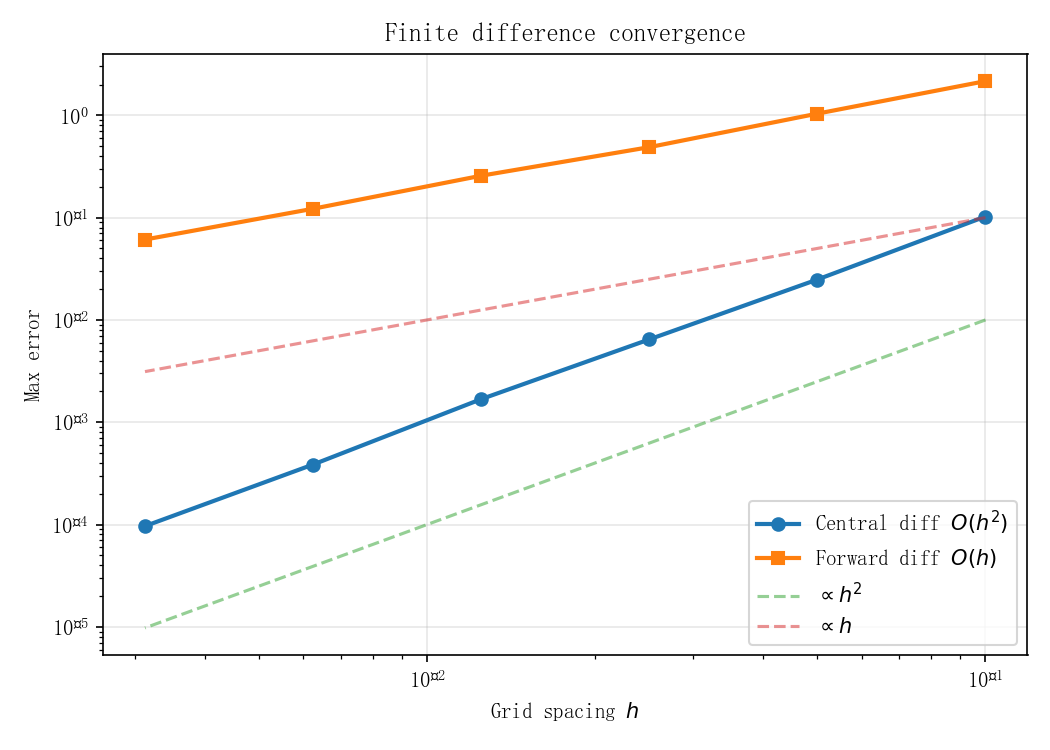
\includegraphics[width=0.6\textwidth]{figures/fig5_3_convergence.png}
\caption{有限差分的收敛性研究。中心差分 $O(h^2)$ 比单侧差分 $O(h)$ 收敛更快。对数坐标下 $O(h^2)$ 的斜率为 2，$O(h)$ 斜率为 1。}
\label{fig:convergence}
\end{figure}

\section{傅里叶变换的数值实现：FFT}
\label{sec:fft}

\subsection{离散傅里叶变换 (DFT)}

对于长度为 $N$ 的序列 $\{f_k\}$：
\begin{equation}
\tilde{f}_n = \sum_{k=0}^{N-1} f_k e^{-2\pi\mathrm{i} nk/N},\qquad
n=0,1,\dots,N-1.
\label{eq:dft}
\end{equation}

直接计算 DFT 需要 $O(N^2)$ 操作。\textbf{快速傅里叶变换 (FFT)} 利用对称性和分治策略将复杂度降至 $O(N\log N)$。

\begin{lstlisting}[language=Python, caption=FFT 频谱分析]
import numpy as np
import matplotlib.pyplot as plt

# 生成信号: 50 Hz 正弦 + 120 Hz 正弦 + 噪声
fs = 1000  # 采样频率 1000 Hz
t = np.arange(0, 1, 1/fs)
f = np.sin(2*np.pi*50*t) + 0.5*np.sin(2*np.pi*120*t)
f += 0.3*np.random.randn(len(t))

# FFT
F = np.fft.fft(f)
freq = np.fft.fftfreq(len(t), 1/fs)

# 单边谱
mask = freq >= 0
plt.figure()
plt.plot(freq[mask], 2*np.abs(F[mask])/len(F))
plt.xlabel('Frequency (Hz)')
plt.ylabel('Amplitude')
plt.xlim(0, 200)
plt.title('FFT Spectrum')
# 预期在 50 Hz 和 120 Hz 处有两个尖峰

# 验证 Parseval 定理
E_time = np.trapz(f**2, t)
E_freq = np.trapz(np.abs(F)**2, freq) / len(F)
print(f"Time-domain energy: {E_time:.4f}")
print(f"Freq-domain energy: {E_freq:.4f}")
print(f"Relative error: {abs(E_time-E_freq)/E_time:.2e}")
\end{lstlisting}

\subsection{FFT 算法原理简述}

FFT 的核心是\textbf{分治策略}（Cooley-Tukey 算法，1965）：

将长度为 $N=2^m$ 的 DFT 分解为两个长度为 $N/2$ 的 DFT：
\begin{equation}
\tilde{f}_n = \sum_{k=0}^{N/2-1} f_{2k} e^{-2\pi\mathrm{i} n(2k)/N}
+ e^{-2\pi\mathrm{i} n/N}\sum_{k=0}^{N/2-1} f_{2k+1} e^{-2\pi\mathrm{i} n(2k+1)/N}.
\end{equation}

递归下去，总操作数从 $N^2$ 降为 $N\log_2 N$。例如 $N=1024$，DFT 需要约 $10^6$ 次操作，FFT 只需约 $10^4$ 次——加速比约 100 倍。

\subsection{用 FFT 求解 PDE}

谱方法利用 FFT 在频域精确计算空间导数，达到谱精度（误差随 $N$ 指数衰减，而非代数衰减）。

\begin{lstlisting}[language=Python, caption=谱方法求解热传导方程]
import numpy as np

def heat_spectral(N=128, T_final=0.1):
    """用 FFT 谱方法求解 u_t = u_xx (周期边界)"""
    L = np.pi
    x = np.linspace(-L, L, N+1)[:-1]  # 周期边界
    h = 2*L / N

    # 初始条件: u(x,0) = sin(x) + 0.5*sin(3*x)
    u0 = np.sin(x) + 0.5*np.sin(3*x)

    # 波数
    k = np.fft.fftfreq(N, h/(2*np.pi))

    # 频域精确解: u_hat(k,t) = u_hat(k,0) * exp(-k^2*t)
    u_hat_0 = np.fft.fft(u0)
    u_hat = u_hat_0 * np.exp(-k**2 * T_final)
    u = np.real(np.fft.ifft(u_hat))

    u_exact = (np.exp(-T_final)*np.sin(x)
               + 0.5*np.exp(-9*T_final)*np.sin(3*x))
    error = np.max(np.abs(u - u_exact))
    return x, u, error

x, u, err = heat_spectral(N=128, T_final=0.1)
print(f"Spectral method error: {err:.2e}")
# 对于光滑解，误差通常在 1e-15 量级（机器精度）
\end{lstlisting}

\begin{insight}
\textbf{谱方法 vs 有限差分：}
\begin{itemize}
\item 光滑解 $\to$ 谱方法（指数收敛，$N=64$ 即可达到机器精度）。
\item 间断解/复杂几何 $\to$ 有限差分或有限元（灵活处理边界和不连续性）。
\item 两者互补：FFT 相当于在傅里叶基下展开（正是第 3 章的内容），有限差分相当于在坐标空间局部近似。
\end{itemize}
\end{insight}

\section{有限元方法初步}
\label{sec:fem_intro}

有限差分法基于微分形式的近似，而\textbf{有限元法 (FEM)} 基于弱形式（积分形式）。FEM 的核心思想是：将解表示为基函数的线性组合，通过加权余量法或变分原理确定系数。

\subsection{一维泊松方程的 FEM 离散}

考虑 $-\frac{\dd^2 u}{\dd x^2} = f(x)$，$u(0)=u(1)=0$。

\textbf{步骤 1：弱形式。} 乘以试函数 $v(x)$ 并分部积分：
\begin{equation}
\int_0^1 u'(x)v'(x)\,\dd x = \int_0^1 f(x)v(x)\,\dd x.
\end{equation}

\textbf{步骤 2：选择基函数。} 将区间分为 $N$ 个单元，每个单元两端为节点。选择\textbf{线性形函数}——在每个单元内为直线，在节点处值为 1，其他节点处为 0：
\begin{equation}
\phi_i(x) = \begin{cases}
\frac{x - x_{i-1}}{h}, & x_{i-1} \leq x \leq x_i,\\
\frac{x_{i+1} - x}{h}, & x_i \leq x \leq x_{i+1},\\
0, & \text{其他}.
\end{cases}
\end{equation}

\textbf{步骤 3：刚度矩阵。} 设 $u(x) = \sum_{j=1}^{N-1} u_j \phi_j(x)$，代入弱形式并取 $v = \phi_i$：
\begin{equation}
\sum_{j=1}^{N-1} u_j \int_0^1 \phi_i'(x)\phi_j'(x)\,\dd x = \int_0^1 f(x)\phi_i(x)\,\dd x.
\end{equation}

计算 $\int \phi_i'\phi_j'\,\dd x$：对 $i=j$，结果为 $2/h$；对相邻节点 $|i-j|=1$，结果为 $-1/h$；其余为 0。这正是有限差分的三对角矩阵！

\begin{insight}
对于一维泊松方程，线性有限元与中心差分有限导出的矩阵完全相同！但 FEM 在处理\textbf{非均匀网格}和\textbf{复杂边界}时更加灵活——自然边界条件（Neumann）在弱形式中自动满足，不需要特殊处理。
\end{insight}

\section{综合案例：有源热传导问题}

\textbf{问题：} 均匀介质中有热源 $f(x) = e^{-50(x-0.3)^2}$（激光加热），左端 $u(0)=0$（接触冷源），右端绝缘 $u_x(1)=0$。求稳态温度分布。

\begin{lstlisting}[language=Python, caption=稳态热传导边值问题]
import numpy as np
from scipy import sparse
from scipy.sparse.linalg import spsolve

def steady_heat_source(N=200):
    """-kappa*u'' = f, u(0)=0, u'(1)=0"""
    kappa = 1.0
    L = 1.0
    h = L / N
    x = np.linspace(0, L, N+1)

    # 热源 (激光加热)
    f = np.exp(-50*(x - 0.3)**2)

    # 构造矩阵 (含 Neumann 边界)
    # 内部点: 标准二阶差分
    # 右边界 u'(1)=0 => u_N = u_{N-1}

    e = np.ones(N+1)
    A = sparse.diags([-e, 2*e, -e], [-1, 0, 1],
                     shape=(N+1, N+1), format='csr') / h**2

    # 左边界 Dirichlet: A[0,:]=0, A[0,0]=1
    A[0, 0] = 1
    A[0, 1] = 0

    # 右边界 Neumann: u'(1)=0 => u_N - u_{N-1}=0
    # 修改最后一行的离散方程
    A[N, N-1] = -1 / h**2
    A[N, N] = 1 / h**2

    # 右端项
    rhs = f.copy()
    rhs[0] = 0  # u(0)=0

    u = spsolve(A, rhs)
    return x, u

x, u = steady_heat_source(N=200)
import matplotlib.pyplot as plt
plt.plot(x, u)
plt.xlabel('x')
plt.ylabel('u(x)')
plt.title('Steady temperature with laser heat source')
# 预期: 热源附近温度最高，向左边界衰减至 0
\end{lstlisting}

\section{本章小结}

\begin{itemize}
\item \textbf{有限差分法} 用泰勒展开近似导数，将 PDE 离散化为代数方程组。
\item \textbf{稀疏矩阵} 是高效求解大规模离散系统的关键——SciPy 提供了 COO/CSR/DIA 等多种格式。
\item \textbf{显式格式} 简单但受 CFL 条件约束；\textbf{隐式格式} 无条件稳定但每步需解线性系统。
\item \textbf{Crank-Nicolson 方法} 结合了两者优点，是时间依赖问题的首选。
\item \textbf{FFT} 在 $O(N\log N)$ 时间内实现傅里叶变换，是谱方法的基石。
\item \textbf{矩阵本征值问题} 直接对应量子力学中的定态薛定谔方程。
\item \textbf{有限元法} 提供比有限差分更强的灵活性和数学基础。
\end{itemize}

\subsection*{概念图谱}

\begin{center}
\fbox{\parbox{0.92\textwidth}{
\textbf{数值方法的概念网络：}\\[3pt]
$\bullet$ 连续 $\to$ 离散：泰勒展开 $\to$ 差分格式\\[3pt]
$\bullet$ 稳态 PDE $\to$ 线性方程组 $Ax=b$ $\to$ 稀疏直接/迭代求解\\[3pt]
$\bullet$ 时间依赖 PDE $\to$ 时间步进 $\to$ 显式（条件稳定）/隐式（无条件稳定）\\[3pt]
$\bullet$ 本征值问题 $\to$ $H\psi=E\psi$ $\to$ Lanczos/ARPACK 迭代\\[3pt]
$\bullet$ 谱方法 $\to$ FFT $\to$ 频域精确导数 $\to$ 指数收敛\\[3pt]
$\bullet$ 有限元 $\to$ 弱形式 $\to$ 刚度矩阵 $\to$ 几何灵活性
}}
\end{center}

\subsection*{公式参考表}

\begin{table}[h]
\centering
\caption{数值方法核心公式速查}
\label{tab:numerical_formulas}
\begin{tabular}{c|c}
\toprule
公式 & 说明 \\
\midrule
$f'(x) \approx \frac{f(x+h)-f(x-h)}{2h}$ & 一阶中心差分 $O(h^2)$ \\
$f''(x) \approx \frac{f(x+h)-2f(x)+f(x-h)}{h^2}$ & 二阶中心差分 $O(h^2)$ \\
$\nabla^2 u_{ij} \approx \frac{u_{i+1,j}+u_{i-1,j}+u_{i,j+1}+u_{i,j-1}-4u_{ij}}{h^2}$ & 五点拉普拉斯格式 \\
$r = \kappa\Delta t/h^2 \leq 1/2$ & 热方程 CFL 条件 \\
$c\Delta t/h \leq 1$ & 波动方程 CFL 条件 \\
$\tilde{f}_n = \sum_{k=0}^{N-1} f_k e^{-2\pi i nk/N}$ & DFT 定义 \\
$O(N\log N)$ vs $O(N^2)$ & FFT vs DFT 复杂度 \\
$E(h) \approx C h^p$ & 收敛性 \\
\bottomrule
\end{tabular}
\end{table}

\begin{insight}[第 5 章的核心思维链条]
\textbf{连续 PDE $\to$ 网格离散 $\to$ 差分近似 $\to$ 稀疏矩阵 $\to$ 代数方程组求解。} 这个链条将前三章的所有解析工具（微分算符、傅里叶变换、特殊函数）统一为可计算的数值框架。你可以将本章看作前三章的"数值镜像"——每当你学到一个新的解析方法，都应该想一想："这个问题的离散版本是什么？对应的矩阵长什么样？"
\end{insight}

\section*{习题}

\textbf{基础题（巩固概念）}

\begin{enumerate}
\item 修改 \texttt{poisson\_1d} 函数，将右端项改为 $f(x)=x(1-x)$，并与解析解 $u(x)=x(1-x)(2-x)/12$ 比较误差。验证误差随 $h$ 以 $O(h^2)$ 衰减。
\item 在 Crank-Nicolson 求解热传导的代码中，观察 $r=0.1, 0.5, 1.0, 5.0$ 时的稳定性。对比显式欧拉法在此 $r$ 值下的表现。
\item 写出五点差分格式 $u_{i+1,j}+u_{i-1,j}+u_{i,j+1}+u_{i,j-1}-4u_{ij}=0$ 的截断误差推导过程，验证其为 $O(h^2)$。
\item 编写一段 Python 代码，用 FFT 生成 200 Hz + 300 Hz 混合信号的频谱图。
\item 利用 \texttt{scipy.sparse.linalg.eigsh} 计算一维无限深势阱的前三个本征函数，并在同一张图上画出数值和解析解的比较。
\item 解释为什么 Crank-Nicolson 格式的精度是 $O(\Delta t^2 + h^2)$，而显式/隐式 Euler 只有 $O(\Delta t + h^2)$。
\end{enumerate}

\textbf{提高题（应用分析）}

\begin{enumerate}
\item[7.] 编程计算一维谐振子 $V(x)=\frac12 x^2$（取 $\hbar=m=\omega=1$）的前 10 个能级，与精确值 $E_n=n+1/2$ 比较。\textbf{提示：} 构造哈密顿矩阵 $H = -\frac12 \frac{\dd^2}{\dd x^2} + \frac12 x^2$ 的离散形式。
\item[8.] 计算 $N=10,20,40,80$ 时二维拉普拉斯方程的解，绘制最大误差随 $N$ 的变化曲线（对数坐标），验证 $O(h^2)$ 收敛。
\item[9.] 设计一个带通滤波器（保留 200 Hz 附近成分），用 FFT 对含噪声信号进行滤波处理。将滤波前后的时域信号和频谱画在同一张图上。
\item[10.] 将一维热传导方程的 FFT 谱方法与 Crank-Nicolson 有限差分法做对比，比较 $N=32,64,128$ 时的计算时间和误差。
\item[11.] 对二维拉普拉斯方程使用不同的迭代求解方法（Jacobi 迭代、Gauss-Seidel 迭代、SOR 方法），比较收敛速度。\textbf{提示：} 对 $M=20$ 的网格，画出误差随迭代步数的变化曲线。
\item[12.] 编写一个函数，利用 Thomas 算法（追赶法）求解三对角系统，并与 \texttt{scipy.sparse.linalg.spsolve} 比较计算时间。
\end{enumerate}

\textbf{挑战题（综合拓展）}

\begin{enumerate}
\item[13.]（二维泊松方程求解器）编写求解 $-\nabla^2 u = f$ 的二维泊松方程求解器（单位正方形区域，$u=0$ 在全部边界上）。右端项取 $f(x,y)=\sin(\pi x)\sin(\pi y)$，解析解为 $u(x,y)=\sin(\pi x)\sin(\pi y)/(2\pi^2)$。验证收敛性。
\item[14.]（薛定谔方程的时间演化）用 Crank-Nicolson 格式离散化时间相关薛定谔方程 $\mathrm{i}\hbar\partial_t\psi = -\frac{\hbar^2}{2m}\partial_x^2\psi$，编写一个演化高斯波包的代码。\textbf{提示：} 这实际上是"虚时间"热传导方程与实时间波动方程的混合——注意 $\mathrm{i}$ 带来的关键区别。
\item[15.]（稀疏矩阵的有限元入门）对一维泊松方程，构造线性有限元刚度矩阵，并与有限差分矩阵对比。说明为何有限元矩阵也是稀疏的，以及它在处理非均匀网格时的优势。
\item[16.]（并行计算的初步认识）将二维拉普拉斯求解器中的矩阵以块形式划分，简要说明如何在多核 CPU 或 GPU 上并行化稀疏矩阵乘法。不需要完整实现，但需要给出伪代码和计算与通信的比例分析。
\item[17.]（自适应网格加密）对于一维泊松方程 $-\frac{\dd^2 u}{\dd x^2}=f(x)$，当 $f(x)$ 在局部区域剧烈变化时，设计一个简单的自适应网格加密策略：在误差大的区域自动加密网格。比较均匀网格和自适应网格的误差与计算量。
\item[18.]（非线性 PDE 的数值求解）考虑一维非线性热传导方程 $u_t = \frac{\partial}{\partial x}\left(k(u)\frac{\partial u}{\partial x}\right)$，其中 $k(u) = 1 + u^2$。用显式格式进行离散化并编写求解程序。说明处理非线性系数的方法。
\end{enumerate}


%------------------ 附录/索引（预留） ------------------
\appendix

\end{document}
